%%%%% --------------------------------------------------------------------------------
%%
%%                               Document Template
%%
%%%%% --------------------------------------------------------------------------------
%% Copyright (C) Huangrui Mo <huangrui.mo@gmail.com>
%% This is free software: you can redistribute it and/or modify it
%% under the terms of the GNU General Public License as published by
%% the Free Software Foundation, either version 3 of the License, or
%% (at your option) any later version.
%%%%% --------------------------------------------------------------------------------
%%
%%%%************************ Document Class Declaration ******************************
%%
\documentclass[doublesided]{Style/ucasthesis}% thesis template of UCAS
%% Multiple optional arguments:
%% [scheme = plain] % for thesis writing of international students
%% [<singlesided|doublesided|printcopy>] % single-sided, double-sided, or print layout
%% [draftversion] % show draft version information, default is no show
%% [fontset = <adobe|...>] % specify font set, default is automatic detection
%% [standard options for ctex class]
%%%%% --------------------------------------------------------------------------------
%%
%%%%************************* Command Define and Settings ****************************
%%
\usepackage[myhdr]{Style/commons}% common settings
%% usage: \usepackage[option1,option2,...,optionN]{commons}
%% Multiple optional arguments:
%% [<numbered|authoryear|alpha>] % citation and reference style
%% <numbered>: textual: Jones [1]; parenthetical: [1]. default style
%% <authoryear>: textual: Jones (1995); parenthetical: (Jones, 1995)
%% <alpha>: textual: not available; parenthetical: [Jon95]
%% [myhdr] % one available header and footer style, will enable fancyhdr
%% [lscape] % provide landscape layout environment
%% [geometry] % configure page layout by geometry package
%% [list] % enable enhanced list environments, useful for Algorithm and Coding
%% [color] % enable color package to use color, default package is xcolor
%% [background] % enable page background, will auto enable color package
%% [tikz] % enable tikz for complex diagrams, will auto enbale color package
%% [table] % enable a table package for complex tables, default is ctable
%% [math] % enable some extra math packages
\usepackage{Style/custom}% user defined commands
%%%%% --------------------------------------------------------------------------------
%\usepackage{xeCJK}

\usepackage{graphicx}
\usepackage{epstopdf}%This is to transfer .eps figure to .pdf figure; please compile your paper using PDFLeTex or PDFTeXify.
 
% 设置图形文件的搜索路径
\graphicspath{{chapter/}{figures/}}

% 取消链接的颜色(黑白打印时)
%\hypersetup{colorlinks=false}

% 小节标题靠左对齐
%\CTEXsetup[format+={\flushleft}]{section}
\newcommand{\R}{\mathbb{R}}
%\newcommand{\C}{\mathbb{C}}
\renewcommand{\i}{\mathbf{i}}
\newcommand{\ii}{\mathbf{i}}
\renewcommand{\Re}{\mathrm{Re}\,}
\renewcommand{\Im}{\mathrm{Im}\,}
\newtheorem{algorithm}{算法}[section]
\newtheorem{lemma}{引理}[section]
\newtheorem{theorem}{定理}[section]
\newtheorem{assumption}{假设}[section]
\newtheorem{remark}{注}[section]
\newtheorem{definition}{定义}[section]
\newtheorem{question}{问题}[section]
\newtheorem{example}{\bf 算例}[section]

\def\debproof{\noindent {\bf 证明.} }
\def\finproof{\hfill {\small $\Box$} \\}

%%%%******************************** Content *****************************************
%%
\begin{document}

%%
%%%%% --------------------------------------------------------------------------------
%%
%%%%******************************** Frontmatter *************************************
%%
%% Frontmatter of Title page, Table of contents, Preface chapter.
\frontmatter
%%
%% >>> Frontpages
%%
%%
%%% >>> Title Page
%%
%%
%%% Chinese Title Page
%%
  \confidential{}% show confidential tag
  \schoollogo{scale=0.112}{UCAS}% university logo
  \title[地球物理反问题的逆时偏移算法]{地球物理反问题的逆时偏移算法}% \title[short title for headers]{Long title of thesis}
  \author{方少峰}% name of author
  \advisor{陈志明~研究员}% names and titles of supervisors
  \advisorinstitute{中国科学院~数学与系统科学研究院}% institute names of supervisors
  \degree{博士}% degree  
  \degreetype{理学}% degree type
  \major{计算数学}% major
  \institute{中国科学院~数学与系统科学研究院}% institute of author
  %\chinesedate{2014~年~06~月}% only need for user customized date
%%
%%% English Title Page
%%
  \englishtitle{Reverse Time Migration Method  \\ in \\ Geophysical Inverse Problem}
  \englishauthor{Fang Shaofeng}
  \englishadvisor{Professor Chen Zhiming}
  \englishdegree{Doctor}
  \englishthesistype{thesis}
  \englishmajor{Computational Mathematics}
  \englishinstitute{Institute of Applied Mathematics \\
    Academy of Mathematics and Systems Science \\
    Chinese Academy of Sciences}
  %\englishdate{June, 2014}% only need for user customized date
%%
%%% Generate Chinese Title
%%
\maketitle
%%
%%% Generate English Title
%%
\makeenglishtitle
%%
%%% >>> Author's declaration
%%
\makedeclaration
%%
%%% >>> Abstract
%%
\chapter{摘\quad 要}% does not show the title on the top
%\begin{abstract}% will show the title on the top
本文主要研究了半空间时谐声波逆散射问题的逆时偏移算法。我们主要关心两个方面,其一是如何利用在半空间表面接收到的无相位数据对嵌入在半空间的障碍物进行成像;其二是以Pekeris开波导模型为例研究半空间分层介质的逆时偏移算法。

在光栅衍射成像和雷达散射成像等问题中,相对于测量相位信息,对数据的模的测量更加易于处理。本文第一部分主要提出了一种半空间无相位数据直接成像算法。 该算法传承了半空间逆时偏移算法的优点,在不需要知道障碍物的任何先验信息的情况下,能够对不同类型的扩展障碍物进行有效成像。通过对新算法成像函数进行分辨率分析,我们证明了当障碍物远离半空间表面时,新算法可以达到和半空间逆时偏移算法相同的精度。最后,我们通过大量的数值算例验证了新算法的有效性和鲁棒性。



在地质勘探及海洋声学成像等领域,被探测的目标大多是嵌入在波导结构中。由于波导模式的存在,波导散射问题和逆散射问题将比在均匀背景介质中复杂地多。本文第二部分主要以Pekeris开波导模型为例研究波在半空间分层介质中的传播性质,以及开波导逆散射问题的逆时偏移算法。通过对点扩散函数的测试和分析,提出了采用Pekeris开波导Dirichlet零边界格林函数进行反传播和计算互相关的开波导逆时偏移算法。数值算例表明,该算法能够对嵌入Pekeris开波导不同介质层的扩展障碍物进行成像。

此外,我们发现在开波导逆时偏移算法中,由于反传播函数和散射数据都会产生波导模式,故而当孔穴半径趋于无穷时,开波导逆时偏移算法的成像函数会产生收敛性问题。为此,我们推导了半空间两层介质阻抗零边界格林函数,并发现若阻抗系数$\lambda$取合理值,则阻抗格林函数函数不会产生波导模式。然后通过对点扩散函数的分析和测试,提出了采用半空间两层介质阻抗零边界格林函数进行反传播和计算互相关的阻抗型开波导逆时偏移算法。数值算例表明,阻抗格林函数可以替代开波导Dirichlet零边界格林函数做为反传播函数,同样可以对障碍物进行有效成像。

\keywords{逆散射问题,逆时偏移算法,无相位数据,Pekeris开波导}
%\end{abstract}


\chapter{Abstract}% does not show the title on the top
%\begin{englishabstract}

\begin{center}
Fang Shao-feng(majored in computational mathematics)

Directed by Prof. Chen Zhi-ming

\end{center}

In this thesis statement, we focus on developing reverse time migration method for time harmonic acoustic wave inverse scattering problems in half space. The first research is to find the support of an unknown extended obstacle embedded in the half space using the amplitude of the total field, while the second one is to study reverse time migration algorithm in Pekeris open waveguide structure.

In the diffractive optics imaging and radar imaging systems, measurement of the intensity of the total field is much easier and cheaper than the phase information of the field. So in the first part, we propose a phaseless directly imaging method for solving the half  space acoustic scattering problem. The new imaging algorithm still holds the advantages of half space reverse time migration method. In fact, it can efficiently find the location of unknown extended obstacles without any priori information. Furthermore, by a detailed analysis of resolution, we prove that the new imaging algorithm can achieve an extraordinary precision, which is the same as the primary one under suitable assumption. The conclusion is also confirmed by a plenty of numerical tests in the end.

It is frequently to see that the target which we are trying to find is embedded in layered medias, such as oil exploration and ocean acoustic imaging. Because of the existence of guided modes, it is much more complicated to solve the waveguide scattering problem and inverse scattering problem. So in the second part, we try to have a clear understanding of how the acoustic wave propagates in open waveguide structure and propose corresponding reverse time migration algorithm, where we  use Pekeris waveguide model as an example. Thanks to the test and analysis of point spread function, we successfully propose the reverse time migration method of open waveguide structure. The algorithm takes the Pekeris open waveguide Dirichlet Green function to compute the processes of back propagation and cross correlation. The numerical examples clearly justify that our algorithm can find the location of obstacles embedded in different layers.

In addition, we are also aware of an interesting and fatal problem in the above open waveguide reverse time migration algorithm. Due to the fact that both back propagation function and waveguide model will emerge many guided modes, the imaging function in the algorithm will not be  absolutely convergent as the aperture radius goes into infinity. Therefore,
we derive the corresponding impedance zero boundary Green function of half space two layered media, and it is delightful to find that the impedance Green function will not emerge guided modes if we choose the impedance parameter properly. Based on this discovery and the test of point spread function, we propose an impedance open waveguide reverse time migration algorithm, which uses impedance Green function to back propagate the scattering data and compute the cross correlation . The numerical tests show that the new algorithm can achieve the same imaging property as the primary one.

\englishkeywords{Inverse scattering problem, Reverse time migration algorithm, Phaseless data, Pekeris open waveguide}
%\end{englishabstract}


%%
%%% >>> List of Content
%%
\intotoc{\contentsname}% add a corresponding item to the contents table and bookmark
\tableofcontents% contents catalog
\intotoc{\listfigurename}% add a corresponding item to the contents table and bookmark
\listoffigures% figures catalog
%\intotoc{\listtablename}% add a corresponding item to the contents table and bookmark
%\listoftables% tables catalog

%%
%% >>> Nomenclatures
%%
\chapter{符号列表}

\section*{符号}
\nomenclatureitem[逆时偏移]{RTM}{Reverse Time Migration}
\nomenclatureitem[全体实数集]{$\R$}{$\{x;-\infty<x<\infty\}$}
\nomenclatureitem[全体复数集]{$\mathbb{C}$}{$\{\xi=\xi_1+\i\xi_2;\xi_1,\xi_2\in\R\}$}
\nomenclatureitem[二维全空间]{$\R^2$}{$\{(x_1,x_2);x_1,x_2\in\R\}$}
\nomenclatureitem[二维半空间]{$\R^2_+$}{$\{(x_1,x_2);x_1\in\R,x_2>0\}$}
\nomenclatureitem[开波导第一层]{$L_1$}{$\{(x_1,x_2);x_1\in\R,0<x_2<h\}$}
\nomenclatureitem[开波导第二层]{$L_1$}{$\{(x_1,x_2);x_1\in\R,x_2>h\}$}
\nomenclatureitem[闭波导区域]{$\R^2_h$}{$\{(x_1,x_2);x_1\in\R,x_2\in(0,h)\}$}
\nomenclatureitem[半空间边界]{$\Gamma_0$}{$\{(x_1,x_2);x_1\in\R,x_2=0\}$}
\nomenclatureitem[开波导间断面]{$\Gamma_h$}{$\{(x_1,x_2);x_1\in\R,x_2=h\}$}
\nomenclatureitem[源点和接收点分布区域]{$\Gamma_0^d$}{$\{(x_1,x_2);x_1\in(-d,d),x_2=0\}$}
\nomenclatureitem[源点在$x_s$处的$\delta$函数]{$\delta_{x_s}(\cdot)$}{}
\nomenclatureitem[频率]{$\omega$}{}
\nomenclatureitem[背景介质速度]{$c,c_1,c_2$}{}
\nomenclatureitem[波数]{$k,k_1,k_2$}{}
\nomenclatureitem[折射系数]{$n(x)$}{}
\nomenclatureitem[阻尼系数]{$\eta(x)$}{}
\nomenclatureitem[第一类零阶Hankel函数]{$H^{(1)}_0(t)$}{}
\nomenclatureitem[第一类一阶Hankel函数]{$H^{(1)}_1(t)$}{}
\nomenclatureitem[波数为$k$的Hemholtz基本解]{$\Phi_k(x,y)$}{$\frac{\i}{4}H^{(1)}_0(k|x-y|)$}
\nomenclatureitem[$y=(y_1,y_2)$关于$\Gamma_0$的镜像点]{$y'$}{$(y_1,-y_2)$}
\nomenclatureitem[$y=(y_1,y_2)$关于$\Gamma_h$的镜像点]{$y^*$}{$(y_1,2h-y_2)$}
\nomenclatureitem[半空间Dirichlet格林函数]{$G_{k}(x,y)$}{$\Phi_{k}(x,y)-\Phi_{k}(x,y')$}
\nomenclatureitem[半空间Neumann格林函数]{$N_{k}(x,y)$}{$\Phi_{k}(x,y)+\Phi_{k}(x,y')$}
\nomenclatureitem[开波导Dirichlet格林函数]{$G(x,y)$}{表达式见定理\ref{f_Dirichlet}和定理\ref{Dirichlet_Mode}}
\nomenclatureitem[开波导Neumann格林函数]{$N(x,y)$}{表达式见定理\ref{f_Neumann}和定理\ref{Neumann_Mode}}
\nomenclatureitem[半空间两层阻抗格林函数]{$G_{\lambda}(x,y)$}{表达式见定理\ref{f_Impedance}}
\nomenclatureitem[全空间两层基本解]{$G_h(x,y)$}{表达式见定理\ref{f_twolayer}}
\nomenclatureitem[闭波导Neumann格林函数]{$N_w(x,y)$}{表达式见式\ref{f_Nw}和引理\ref{mode_Nw}}
\nomenclatureitem[闭波导Dirichlet格林函数]{$G_w(x,y)$}{表达式见式\ref{f_Gw}和引理\ref{mode_Gw}}
\nomenclatureitem[点扩散函数]{$J(z,y)$}{}
\nomenclatureitem[有限孔穴点扩散函数]{$J_d(z,y)$}{}
\nomenclatureitem[障碍物]{$D$}{一个有界的Lipschitz区域}
\nomenclatureitem[$D$上的Lebesgue可积函数集]{$L^1(D)$}{$\left\{f(x);\int_D|f(x)|dx<+\infty\right\}$}
\nomenclatureitem[$D$上的平方可积函数集]{$L^2(D)$}{$\left\{f(x);\int_D|f(x)|^2dx<+\infty\right\}$}
\nomenclatureitem[$D$上的$H^1$函数集]{$H^1(D)$}{$\left\{f(x);f,\nabla f\in L^2(D)\right\}$}
\nomenclatureitem[$D$上的本质有界函数集]{$L^{\infty}(D)$}{$\{f(x);esssup |f(x)|<+\infty\}$}
\nomenclatureitem[采样区域]{$\Omega$}{}
\nomenclatureitem[函数$f$在界面$\Gamma_h$处的跳量]{$[f(\cdot)]_{\Gamma_h}$}{}





\mainmatter

\chapter{引言}\label{chap:fundamental}

近几十年来,在实际问题的驱动下,数学物理反问题已经成为应用数学领域中成长的最快的领域之一。这得益于数学物理反问题在石油勘探、遥感技术、医疗成像、信号处理以及雷达散射成像等众多科学技术领域当中的广泛应用。地球物理反问题是数学物理反问题中比较活跃的分支之一,其基本思想是通过对观测数据进行分析,来预测或估计地下介质的几何结构和物理参数信息。散射问题以声波、电磁波以及弹性波三类波动方程为模型来解释波在介质中传播的各种物理现象,而与之相对应的逆散射问题则在地球物理反问题的科学研究和实际应用中起到至关重要的作用。逆散射问题应用价值较大,但又具有强非线性和高度不适定性的特性,于是关于逆散射问题的理论研究和数值重构算法非常富有挑战性和吸引力。在众多应用数学家的努力下,很多难点被攻克,尤其是以全空间为背景模型的散射问题和逆散射问题研究。然而,在勘探地球物理反问题当中,欲探寻的目标距离地表较远,且地下大多是分层介质的复杂结构,于是以全空间为数学模型有时并不能对实际问题做到很好地刻画。故而本文在前人研究的基础上,对一般半空间以及半空间分层介质上的散射问题和逆散射问题加以研究,特别是考虑如何从数值上构造高效稳定的成像重构算法。在本章,我们将首先简单介绍一下声波半空间上的散射问题和逆散射问题,然后再介绍两种常见的波导结构以及相应的散射问题和逆散射问题。
\section{声波半空间散射问题与逆散射问题}
地球表面是一个特殊的分界面,它将介质划分为两个半空间,地面以上为空气介质,其密度与地面以下的岩石或者海平面以下的海水层相比可以忽略,故而以半空间为模型来研究散射问题和逆散射问题具有重要的应用价值。

令障碍物$D$为我们的成像目标,且$D$嵌入在背景介质速度为常数$c_0$的均匀半空间$\R^2_+$当中,其中$\R^2_+=\{(x_1,x_2)^T:x_1\in\R,x_2>0\}$. 我们假设$D$是一个有界的Lipschitz 区域,其边界记为 $\Gamma_D$. 若$D$为可穿透障碍物,则在半空间中,时谐声波波场$u(x,x_s)$满足如下Hemholtz方程和边界条件:
\begin{eqnarray}
 \Delta_x u(x,x_s)+k^2n(x)u(x,x_s)=-\delta_{x_s}(x),&in&\R^2_+   \label{into_p1_1}\\
 \frac{\partial u(x,x_s)}{\partial x_2}=0,&on&\Gamma_0  \label{into_p1_2}
\end{eqnarray}

其中$\omega$为频率,$k=\frac{\omega}{c_0}>0$为波数,$c(x)$表示波在介质中的传播速度以及$n(x)=\frac{c_0^2}{c^2(x)}$为折射系数的平方。此外,$x_s$为点源激发的位置,$\Gamma_0=\{(x_1,x_2)^T:x_1\in\R,x_2=0\}$表示半空间的边界。

为了保证方程\eqref{into_p1_1}-\eqref{into_p1_2}具有物理意义解的唯一性,$u(x,x_s)$在无穷远处需要满足著名的Sommerfeld辐射条件:
\begin{equation}\label{into_p1_3}
  \sqrt{r}\left(\frac{\partial u}{\partial r}-\i k u\right)\rightarrow0\ \ as\ \ r=|x|\rightarrow\infty
\end{equation}

令$N_k(x,y)$为满足如下方程的声波半空间Neumann格林函数:
\begin{eqnarray}
\left\{
\begin{array}{lll}
 \Delta_x N_k(x,y)+k^2N_k(x,y)=-\delta_{y}(x),&in&\R^2_+   \label{into_p2_1}\\
 & &\\
 \frac{\partial N_k(x,y)}{\partial x_2}=0,&on&\Gamma_0  \label{into_p2_2}\\
 & &\\
 \sqrt{r}\left(\frac{\partial N_k}{\partial r}-\i k N_k\right)\rightarrow0,&as&r=|x|\rightarrow\infty\label{into_p2_3}
\end{array}
\right.
\end{eqnarray}
直接验证可知
\begin{equation}
  N_k(x,y)=\Phi_{k}(x,y)+\Phi_{k}(x,y')
\end{equation}
其中$\Phi_k(x,y)=\frac{\i}{4}H_0^{(1)}(k|x-y|)$是波数为$k$的Hemholtz方程基本解,$y'=(y_1,-y_2)$ 是 $y=(y_1,y_2)\in\R^2_+$关于$\Gamma_0$的镜像点。


若令$u^i(x,x_s)$为在点源$x_s$处激发而产生的入射场,则$u^i(x,x_s)=N_k(x,x_s)$,从而散射场$u^s(x,x_s)=u(x,x_s)-u^i(x,x_s)$满足如下方程:
\begin{eqnarray}\label{half_scatter}
\left\{
\begin{array}{lll}
 \Delta u^s(x,x_s)+k^2u^s(x,x_s)=k^2[1-n(x)]u(x,x_s),&in&\R^2_+   \label{into_p3_1}\\
 & &\\
 \frac{\partial u^s(x,x_s)}{\partial x_2}=0,&on&\Gamma_0  \label{into_p3_2}\\
 & &\\
 \sqrt{r}\left(\frac{\partial u^s}{\partial r}-\i k u^s\right)\rightarrow0,&as&r=|x|\rightarrow\infty\label{into_p3_3}
\end{array}
\right.
\end{eqnarray}

类似地,我们可以考虑当散射体$D$为不可穿透障碍物时散射场所满足的方程。当障碍物不可穿透时,总场$u(x,x_s)$ 满足如下方程:
\begin{eqnarray}
\left\{
\begin{array}{lll}
 \Delta u(x,x_s)+k^2u(x,x_s)=-\delta_{x_s}(x),&in&\R^2_+\backslash\overline{D}   \label{into_p4_1}\\
 & &\\
 \frac{\partial u(x,x_s)}{\partial x_2}=0,&on&\Gamma_0  \label{into_p4_2}\\
 & &\\
 \sqrt{r}\left(\frac{\partial u}{\partial r}-\i k u\right)\rightarrow0,&as& r=|x|\rightarrow\infty\label{into_p4_3}
\end{array}
\right.
\end{eqnarray}

此外,我们还要对不同类型的不可穿透障碍物添加上合适的边界条件,具体如下:
\begin{itemize}
  \item 声软障碍物:
  \begin{equation}
     u=0,\ \ on\ \ \Gamma_D
  \end{equation}
  \item 声硬障碍物:
  \begin{equation}
    \frac{\partial u(x,x_s)}{\partial\nu}=0,\ \ on\ \ \Gamma_D
  \end{equation}
  \item 阻抗障碍物:
  \begin{equation}
    \frac{\partial u(x,x_s)}{\partial\nu}+\i k\eta(x)u(x,x_s)=0,\ \ on\ \ \Gamma_D
  \end{equation}
\end{itemize}
 这里$\eta(x)$为障碍物$D$的阻抗系数。

从而对于声软障碍物来说,散射场$u^s(x,x_s)=u(x,x_s)-u^i(x,x_s)$满足如下方程:
\begin{eqnarray}
\left\{
\begin{array}{lll}
 \Delta u^s(x,x_s)+k^2u^s(x,x_s)=0,&in&\R^2_+\backslash\overline{D}  \\
 & &\\
 \frac{\partial u^s(x,x_s)}{\partial x_2}=0,&on&\Gamma_0  \\
 & &\\
 u^s(x,x_s)=-N_k(x,x_s),& on&\Gamma_D\\
 & &\\
 \sqrt{r}\left(\frac{\partial u^s}{\partial r}-\i k u^s\right)\rightarrow0,&as&r=|x|\rightarrow\infty
\end{array}
\right.
\end{eqnarray}

对于声硬障碍物和阻抗障碍物,只须将在障碍物边界$\Gamma_D$上的边界条件分别换为
\begin{equation}
  \frac{\partial u^s(x,x_s)}{\partial\nu}=-\frac{\partial N_k(x,x_s)}{\partial\nu}
\end{equation}
和
\begin{equation}
  \frac{\partial u^s(x,x_s)}{\partial\nu}+\i k\eta(x)u^s(x,x_s)=-\left(\frac{\partial N_k(x,x_s)}{\partial\nu}+\i k\eta(x)N_k(x,x_s)\right)
\end{equation}
于是半空间散射问题即可定义如下:
\begin{question}[半空间散射问题]
$(i).$ 可穿透障碍物散射问题:
    已知障碍物位置、大小、形状和折射系数,求解散射场$u^s(x,x_s)$。\\
$(ii).$ 不可穿透障碍物散射问题:
    已知障碍物位置、大小、形状、边界类型和阻抗系数,求解散射场$u^s(x,x_s)$。
\end{question}

关于一般全空间声波散射问题的适定性的研究已经很完善,详见文献David Colton\cite{colton-kress,Cakoni2014A}和
William Mclean\cite{Mclean2000Strongly}。关于声波半空间散射问题适定性研究的文献也有很多,例如文献Zhang Bo\cite{Bo1998Acoustic},Simon N.Chandler-Wilde\cite{Chandler1996Scattering,Chandler1997The}。特别地,我们参考了
文献\cite{ch_ha}中关于声波半空间声软障碍物的适定性结果,其证明方法是利用经典的极限吸收原理,具体可参考文献
Rolf Leis\cite{Leis1986Initial}和Zhiming Chen\cite{cz2010,ch_cw}。


在本文中,我们主要对半空间上的逆散射问题感兴趣,特别是关于障碍物成像问题的数值重构算法。假设我们不知道障碍物的任何先验信息,包括障碍物是否可穿透以及$u(x,x_s)$在障碍物边界上所满足的边界条件,然后我们研究的问题具体如下:
 \begin{question}[半空间障碍物成像问题]\label{ques_half}
$(i).$   在远离障碍物的区域上采集散射数据$u^s(x,x_s)$或总场数据$u(x,x_s)$,通过数值重构算法确定出障碍物的位置、大小和形状。\\
$(ii).$  在远离障碍物的区域上采集无相位散射数据$|u^s(x,x_s)|$或总场数据$|u(x,x_s)|$,通过数值重构算法确定出障碍物的位置、大小和形状。
 \end{question}

 求解障碍物成像问题的方法主要分为两大类:直接成像法和迭代法。直接成像法主要是通过分析问题的本质特征,构造出一个直接成像函数,该函数通过对接收到的散射数据加以处理,可以直接对障碍物进行成像。具体而言,当采样点靠近障碍物边界时,成像函数呈现峰值;当采样点远离障碍物时,成像函数逐渐衰减,于是直接成像法不需要迭代求解正散射问题,就可以确定障碍物的位置、大小和形状。迭代法主要是将原始问题化成一个优化问题,通过建立目标函数,选取合适的数值优化算法,然后不断迭代来确定最优的参数,再代入原始问题。在一定条件下,迭代法能够较好地确定障碍物的位置和形状,甚至关于介质参数的定量信息。然而迭代法的收敛性和实用性却有待考量。首先,迭代法的收敛性分析极为复杂;其次,迭代法的收敛需要一个较好地初值,这就需要关于障碍物一定的先验信息;最后,由于迭代法每一步迭代都需要求解一个正散射问题,计算极为耗时,且十分依赖正散射问题的求解精度。因此,本文主要关注于如何构造求解障碍物成像问题的直接成像算法。特别地,我们主要研究了在实际当中应用广泛的一种直接成像算法,即逆时偏移成像算法。下面我们简单地对该算法做一个介绍。

%常见的迭代法和直接成像法介绍

\section{逆时偏移算法思想介绍}

逆时偏移成像算法(Reverse Time Migration)是一种直接成像法,由于其能够对复杂地质构造直接进行有效成像,因而在勘探地球物理反问题领域得到了广泛的应用,
%具体可参看文献
同时也引起了很多学者对其理论分析的研究
%,例如文献中基于高频渐进假设或者几何光学近似进行了渐进分析。
。文献Zhiming Chen\cite{cch_a}中,针对全空间时谐声波逆散射问题,首次提出了频率域单频逆时偏移成像算法,并且基于Hemholtz-Kirchhoff 恒等式,对成像函数建立了严格的分辨率分析。紧接着,他们在文献\cite{cch_e}中针对全空间电磁波逆散射问题,提出了新的单频电磁波逆时偏移算法;在文献\cite{ch_e}中针对全空间弹性波逆散射问题,提出新的单频弹性波逆时偏移算法,并且基于类似的Hemholtz-Kirchhoff恒等式,均建立了严格的分辨率分析。文献\cite{cch_a,cch_e,ch_e}分别针对声波、电磁波和弹性波逆散射问题提出的算法和理论构成了逆时偏移算法的数学理论基础。特别地,其所提算法的分辨率分析不需要高频渐进假设或几何光学近似,这是一个极大地进展。

在文献\cite{ch_cw}中,Zhiming Chen等人考虑了平板声波波导逆散射问题,提出了广义的Hemholtz-Kirchhoff恒等式,并以此为出发点构造了声波闭波导逆时偏移算法。然后他们在文献\cite{ch_ha}中对半空间时谐声波逆散射问题进行研究时,发现半空间模型下Hemholtz-Kirchhoff恒等式不再成立,于是其引入了点扩散函数,并通过对点扩散函数的分析建立了半空间声波逆时偏移算法的分辨率分析。
我们强调,点扩散函数的引入对于求解一般半空间模型以及半空间分层介质上的逆散射问题,有着至关重要的作用。

由于逆时偏移算法简单而有效、数值实现容易以及可扩展性较好,故而本文将从文献\cite{ch_ha}出发,继续对此算法进行研究。文献
\cite{ch_ha}中的算法主要是为解决问题\ref{ques_half}中的第一部分而提出的,算法所使用的的数据为散射场$u^s(x,x_s)$的所有信息。本文第二章将考虑对其加以改进以适用于问题\ref{ques_half}中的第二部分,使得改进后的算法仅需要利用总场的振幅信息即可。
逆时偏移算法的思想很简单,主要分为两步:计算反传播场和互相关关系,具体如下所示:
\begin{algorithm}
设$d>0$为孔穴半径,在$\Gamma_0^d:=\{(x_1,x_2);x_1\in(-d,d),x_2=0\}$上均匀分布着$N_s$个源点$x_s$和$N_r$个接收点$x_r$,其中
$s=1,2,\ldots,N_s;r=1,2,\ldots,N_r$。令$u^s(x_r,x_s)$为在接收点$x_r$处记录的由源点$x_s$激发而产生的散射场,以及区域$\Omega$为采样区域。然后对任意地$z\in\Omega$,计算反传播场和互相关关系:\\
$1^\circ$ 反传播: 对于 $s=1,\ldots,N_s$, 计算反传波场
\begin{equation}
  v_b(z,x_s)=\frac{|\Gamma_0^d|}{N_r}\sum\limits_{r=1}^{N_r}\frac{\partial\Phi_k(x_r,z)}{\partial x_2(x_r)}u^s(x_r,x_s),\  \  \forall z\in\Omega.
\end{equation}
$2^\circ$ 互相关: 对于 $z\in\Omega$, 计算成像函数
\begin{equation}
  I_d(z)=\Im\left\{\frac{|\Gamma_0^d|}{N_s}\sum\limits_{s=1}^{N_s}\frac{\partial\Phi_k(x_s,z)}{\partial x_2(x_s)}v_b(z,x_s)
  \right\}.
\end{equation}
将反传波场$v_b(z,x_s)$代入到成像函数$I_d(z)$,可得
\begin{equation}
  \qquad I_d(z)=\Im\left\{\frac{|\Gamma_0^d||\Gamma_0^d|}{N_sN_r}
  \sum\limits_{s=1}^{N_s}\sum\limits_{r=1}^{N_r}
  \frac{\partial\Phi_k(x_s,z)}{\partial x_2(x_s)}\frac{\partial\Phi_k(x_r,z)}{\partial x_2(x_r)}
  u^s(x_r,x_s)
  \right\},\  \ \forall z\in\Omega.\quad\quad
\end{equation}
若令$N_s,N_r\rightarrow\infty$,则上式可看做对如下积分的近似:
\begin{equation}
 \qquad  I_{\rm RTM}(z)=\Im\int_{\Gamma_0^d}\int_{\Gamma_0^d}\frac{\partial\Phi_k(x_s,z)}{\partial x_2(x_s)}\frac{\partial\Phi_k(x_r,z)}{\partial x_2(x_r)}
  u^s(x_r,x_s)ds(x_r)ds(x_s),\  \  \forall z\in\Omega.\quad\quad
\end{equation}
\end{algorithm}

与文献\cite{cch_a,cch_e,ch_e,ch_cw}不同,半空间模型下的Hemholtz-Kirchhoff恒等式不再成立。文献\cite{ch_ha}中成像函数$I_{\rm RTM}(z)$ 的分辨率分析主要是基于对其所定义半空间点扩散函数的分析。声波半空间点扩散函数$J(z,y)$定义如下:
\begin{equation}\label{psf_chha}
  J(z,y)=\int_{\Gamma_0}\frac{\partial G_{k}(x,z)}{\partial x_2}\overline{N_{k}(x,y)}ds(x)
\end{equation}
其中$G_{k}(x,y),N_{k}(x,y)$分别是波数为$k$的半空间Dirichlet零边界和Neumann零边界格林函数,具体如下
\begin{equation}
G_{k}(x,y)=\Phi_{k}(x,y)-\Phi_{k}(x,y'),\ \ N_{k}(x,y)=\Phi_{k}(x,y)+\Phi_{k}(x,y')
\end{equation}
\begin{figure}[htbp]
  \centering
  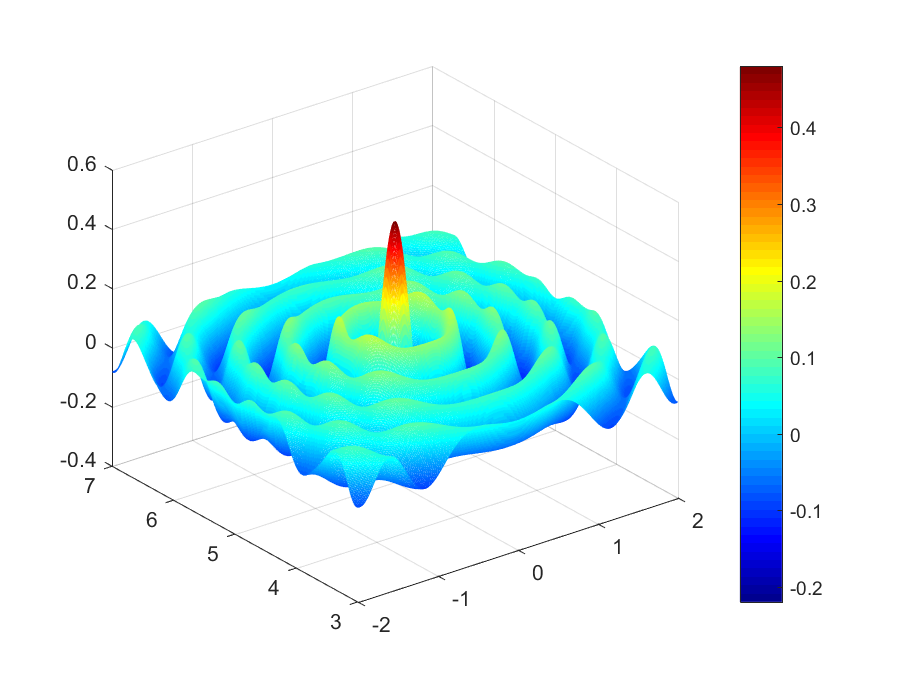
\includegraphics[width=0.8\textwidth]{./intro/psf_chha.eps}
  \caption{$-\Im J(z,y)$,其中$k=4\pi,y=(0,5),z\in[-2,2]\times[3,7]$}\label{fig_psf_chha}
\end{figure}

点扩散函数$J(z,y)$具有如下性质:当$z=y$时,$-\Im J(z,y)$会取得峰值;当$z$逐渐远离$y$点时,$-\Im J(z,y)$会逐渐衰减,具体表现如图\ref{fig_psf_chha}所示。根据文献\cite{ch_ha}中的分析可知,正是由于点扩散函数$J(z,y)$具备如此的性质,才使得成像函数$I_{\rm RTM}(z)$ 对障碍物能够有效成像。受此启发,我们在求解Pekeris开波导障碍物成像问题时,同样可以从点扩散函数出发来选择合适的反传播函数,进而确定适用于Pekeris开波导逆散射问题的逆时偏移算法,详细内容将在第三章和第四章进行讨论。

\section{波导模型初步介绍}
在地球物理反问题当中,被探测的目标大多是嵌入在分层介质当中的,故而近年来以分层介质为背景模型的散射问题和逆散射问题引起了极大地关注。与均匀介质不同,介质的层状结构使得波的传播和散射问题研究变得极为复杂,尤其是波导现象的出现。这导致与之相应的障碍物成像问题也变得较为棘手,很多数值重构算法无法直接加以推广。在本节中,我们将简要地介绍平板声波闭波导和Pekeris开波导模型。

\subsection{平板声波闭波导}
与半空间模型不同,平板声波闭波导除边界$\Gamma_0=\{(x_1,x_2)^T:x_1\in\R,x_2=0\}$之外,还有一个边界$\Gamma_h=\{(x_1,x_2)^T:x_1\in\R,x_2=h\}$。两个边界之间的区域记为$\R^2_h=\{(x_1,x_2)^T:x_1\in\R,x_2\in(0,h)\}$,其被称为波导区域。在波导区域中,时谐声波总场满足Hemholtz方程,且在边界$\Gamma_0$和$\Gamma_h$上分别满足Dirichlet 和Neumann 边界条件,
\begin{eqnarray}\label{cwg}
\left\{
\begin{array}{lll}
   \Delta_x u(x,x_s)+k^2u(x,x_s)=-\delta_{x_s}(x),& in&\R^2_h\backslash\overline{D}\\
   & &\\
   u(x,x_s)=0,& on&\Gamma_0\\
   & &\\
   \frac{\partial u(x,x_s)}{\partial x_2}=0,& on&\Gamma_h\\
   & &\\
   \frac{\partial u(x,x_s)}{\partial\nu}+\i k\eta(x)u(x,x_s)=0,& on&\Gamma_D
\end{array}
\right.
\end{eqnarray}
其中$D$为阻尼系数为$\eta(x)$的阻抗障碍物。类似地,我们可以定义其他边界类型的障碍物和可穿障碍物散射方程。

为保证方程\eqref{cwg}具有物理意义解的唯一性,还需要为其添加合适的辐射条件。设障碍物$D\subset B_R:=(-R,R)\times(0,h)$,其中$R>0$,则由分离变量法可知$u_{x_s}(x_1,x_2):=u(x,x_s)$具有如下模式展开表达式:
\begin{equation}
  u_{x_s}(x_1,x_2)=\sum\limits_{n=1}^{\infty}u_n(x_1)\sin(\mu_nx_2),\ \ \forall |x_1|>R
\end{equation}
其中$u_n(x_1),n=1,2,\cdots,$ 为模式展开系数函数,其满足如下1D的Hemholtz方程:
\begin{equation}\label{cwg_mec}
  u''_n+\xi^2_nu_n=0,\ \ \forall |x_1|>R,\ \ n=1,2,\cdots,
\end{equation}
和辐射条件
\begin{equation}\label{cwg_rad}
 \lim\limits_{|x_1|\rightarrow+\infty}\left(\frac{\partial u_n}{\partial|x_1|}-\i\xi_nu_n\right)=0,\ \ n=1,2\cdots,
\end{equation}
其中,$\mu_n=\frac{2n-1}{2h}\pi,n=1,2,\cdots,$为闭波导模型的截断频率,以及
\begin{eqnarray}
 \xi_n=\left\{
\begin{array}{lll}
   \sqrt{k^2-\mu_n^2}&,&\mu_n<k\\
   \sqrt{\mu_n^2-k^2}&,&\mu_n>k
\end{array}
\right.
\ \ \ n=1,2,\cdots,
\end{eqnarray}
此外,在闭波导模型中,我们总假设波数不等于截断频率,即
\begin{equation}
  k\neq\frac{2n-1}{2h}\pi,n=1,2,\cdots.
\end{equation}

辐射条件\eqref{cwg_rad}保证了1维Hemholtz方程\eqref{cwg_mec}的唯一性,且方程\eqref{cwg}联合辐射条件\eqref{cwg_rad}构成了
闭波导阻抗障碍物散射问题。关于该闭波导散射问题的适定性的研究的文献还有很多,例如
Arens\cite{Arens2010Variational,Arens2011Direct},Morgenr$\ddot{o}$ther\cite{K1988On,K2010on}和 Yongzhi Xu\cite{Xu1990The}。闭波导模型适定性分析的主要困难在于陷阱模式(Embedded Trapped Modes)的存在破坏了散射问题的唯一性,具体分析可见文献\cite{Linton2013Embedded}。当障碍物为如方程\eqref{cwg}中所示的阻抗障碍物时,文献\cite{ch_cw}证明了散射问题的唯一性,并通过极限吸收原理完成了存在性的证明。若障碍物为其他边界类型,由于陷阱模式(Embedded Trapped Modes)的存在,闭波导障碍物散射问题的唯一性并不一定能够得到保证。

\subsection{Pekeris开波导}

在1948年,Pekeris首次提出了半空间两层介质的开波导模型,故而我们称其为Pekeris开波导模型。设$c_0(x)$ 为背景介质速度:
\begin{eqnarray*}
c_0(x)=\left\{
 \begin{array}{lll}
   c_1&,&x\in L_1\\
   c_2&,&x\in L_2
 \end{array}
\right.
\end{eqnarray*}
其中$L_1=\{(x_1,x_2)\in\R^2;x_1\in\R,x_2\in(0,h)\}$表示第一层介质,$h$为第一层介质的厚度,$L_2=\{(x_1,x_2)\in\R^2;x_1\in\R,x_2\in(h,\infty)\}$表示第二层介质。当$c_1=c_2$时,该模型退化为一般的半空间情形;当$c_1>c_2$时,该模型不会产生波导现象;当$c_1<c_2$时,该模型才会产生波导,故而在本文我们仅考虑$c_1<c_2$的情形。令$\Gamma_0=\{(x_1,x_2)^T:x_1\in\R,x_2=0\}$依旧表示半空间的边界,而$\Gamma_h=\{(x_1,x_2)^T:x_1\in\R,x_2=h\}$表示两层介质的
分界面,第一层$L_1$表示波导区域。以可穿透障碍物散射问题为例,类似于半空间均匀背景介质情形,声波波场$u(x,x_s)$满足如下Hemholtz方程和边界条件:
\begin{eqnarray}
 \Delta u(x,x_s)+k^2(x)n(x)u(x,x_s)=-\delta_{x_s}(x),&in&\R^2_+   \label{into_q1_1}\\
 \frac{\partial u(x,x_s)}{\partial x_2}=0,&on&\Gamma_0  \label{into_q1_2}
\end{eqnarray}
其中$\omega$仍表示频率,$c(x)$仍表示波在介质中的传播速度,折射系数$n(x)=\frac{c_0^2(x)}{c^2(x)}$,以及波数$k(x)=\frac{\omega}{c_0(x)}$,即:
\begin{eqnarray*}
k(x)=\left\{
 \begin{array}{lll}
   k_1&,&x\in L_1\\
   k_2&,&x\in L_2
 \end{array}
\right.
\end{eqnarray*}
其中$k_1=\frac{\omega}{c_1},k_2=\frac{\omega}{c_2}$。 易知$k_1>k_2$, 这保证了波导现象的产生。
除此之外,$u(x,x_s)$在分界面$\Gamma_h$处还需满足如下连续性条件:
\begin{eqnarray}
 \left[u(\cdot,x_s)\right]_{\Gamma_h}=0,\ \ \left[\frac{\partial u(\cdot,x_s)}{\partial\nu}\right]_{\Gamma_h}=0 \label{into_q1_3}
\end{eqnarray}

设$u^i(x,x_s)$为点源在$x_s$处激发产生的入射场,则$u^i(x,x_s)=N(x,x_s)$,其中$N(x,y)$为点源在
y处激发而产生的Pekeris开波导Neumann零边界格林函数,它满足如下方程:
\begin{eqnarray}
\left\{
\begin{array}{lll}
  \Delta_xN(x,y)+k^2(x)N(x,y)=-\delta_y(x),&in&\R^2_+\\
  & &\\
  \left[N(\cdot,y)\right]_{\Gamma_h}=0,\ \ \left[\frac{\partial N(\cdot,y)}{\partial\nu}\right]_{\Gamma_h}=0 & &\\
  & &\\
  \frac{\partial N(x,y)}{\partial x_2}=0, &on&\Gamma_0
\end{array}
\right.
\end{eqnarray}
于是散射场$u^s(x,x_s)=u(x,x_s)-u^i(x,x_s)$满足如下方程:
\begin{eqnarray}
\left\{
\begin{array}{lll}
 \Delta u^s(x,x_s)+k^2(x)u^s(x,x_s)=k^2[1-n(x)]u(x,x_s),&in&\R^2_+   \label{into_q3_1}\\
 & &\\
 \frac{\partial u^s(x,x_s)}{\partial x_2}=0,&on&\Gamma_0  \label{into_q3_2}\\
 & &\\
 \left[u^s(\cdot,x_s)\right]_{\Gamma_h}=0,\ \ \left[\frac{\partial u^s(\cdot,x_s)}{\partial\nu}\right]_{\Gamma_h}=0 \label{into_q3_3}
\end{array}
\right.
\end{eqnarray}

类似地,我们可以定义Pekeris开波导不可穿透障碍物散射问题,总场$u(x,x_s)$满足如下方程
\begin{eqnarray}
\left\{
\begin{array}{lll}
 \Delta u(x,x_s)+k^2u(x,x_s)=-\delta_{x_s}(x),&in&\R^2_+\backslash\overline{D}   \label{into_q4_1}\\
 & &\\
 \frac{\partial u(x,x_s)}{\partial x_2}=0,&on&\Gamma_0  \label{into_q4_2}\\
 & &\\
 \left[u(\cdot,x_s)\right]_{\Gamma_h}=0,\ \ \left[\frac{\partial u(\cdot,x_s)}{\partial\nu}\right]_{\Gamma_h}=0 \label{into_q4_3}
\end{array}
\right.
\end{eqnarray}
以及分别针对声软,声硬和阻抗障碍物的三种边界条件:
\begin{eqnarray}
 u=0,\ \ \frac{\partial u}{\partial\nu}=0,\ \ \frac{\partial u}{\partial\nu}+\i k(x)\eta(x)u=0,&on&\Gamma_D
\end{eqnarray}

开波导模型具有广泛的应用价值,故而引起了很多应用数学家的关注和研究,并提出了很多辐射条件以保证开波导散射问题的唯一性和存在性。例如文献Ciraolo和Magnanini\cite{Ciraolo2009A1,Ciraolo2009A2},Bonnet-Ben
Dhia和Christophe Hazard\cite{Dhia2009DIFFRACTION},以及Nedelec\cite{Jerez2012Asymptotics}。类似于闭波导情形,开波导模型同样会产生波导模式和衰减项,辐射条件需要对这两种模式分别进行考虑。与闭波导不同的是,开波导横向和纵向都可以趋于无穷远,而波在这两个方向的传播性质完全不同,故而开波导的分析比闭波导要复杂的多。有意思的是,开波导模型并不会出现类似于闭波导模型下的陷阱模式(Embedded Trapped Modes),该结论的证明可以参考文献\cite{Littman1982Spectral,Weder1988Absence,Hazard2014On}。


我们将在本文第三章以Pekeris开波导模型为例对开波导散射问题和逆散射问题进一步探讨和研究。
而且我们更关心的是如何提出高效准确的数值重构算法,以解决Pekeris开波导模型障碍物成像问题,也就是如下问题:
\begin{question}
 如何通过测量到的散射数据$u^s(x,x_s)$,建立快速有效的数值重构算法,确定嵌入在开波导结构中的障碍物$D$的大小、位置和形状。
\end{question}

如果一个障碍物$D$嵌入在波导结构中,那么想要确定其位置、大小和形状,则会因为波导模式的影响而远比均匀背景介质模型要棘手。关于闭波导逆散射问题的研究已经有很多成熟的算法,例如Arens\cite{Arens2011Direct}和Zhiming Chen
\cite{ch_cw}。对于开波导逆散射问题,也有一些研究结果,例如Robert Gilbert\cite{Gilbert2007Inverse}在一定假设下证明了可穿透障碍物逆散射问题的唯一性;Habib Ammari\cite{Ammari2005Reconstruction}提出了MUSIC 型算法,当障碍物的尺寸比较小时,该算法能够较好确定其位置;Gang Bao\cite{Bao2013Reconstruction}同样对开波导障碍物成像问题的唯一性进行了研究,其唯一性结论需要采集多个频率的远场数据,此外他们还计划将文献
\cite{Bao2005Inverse,Bao2010Error,Bao2011An}中提到的逐步线性化方法推广到开波导模型。

文献\cite{ch_cw}针对平板声波闭波导障碍物成像问题提出了闭波导逆时偏移算法,本文计划将其推广到Pekeris开波导情形,并分析和讨论闭波导和开波导模型有何区别,以及由此而产生的一些有意思的问题和现象。

\newpage
\section{本文主要工作}

本文主要研究了一般半空间以及半空间分层介质上障碍物成像问题的逆时偏移成像算法。文章具体内容安排如下:

第二章主要研究一般的声波半空间障碍物成像问题,在文献\cite{ch_ha}中半空间声波逆时偏移算法的基础上,提出了一种新型的直接成像算法。该算法不需要利用散射场的相位数据信息,仅仅使用总场的振幅数据即可对障碍物进行成像。与此同时,该算法不需要提前知道障碍物的任何先验信息,例如障碍物是否可穿透,以及不可穿透障碍物的边界条件。然后我们通过对新算法成像函数的分辨率分析,证明了在一些合理的假设下,新算法可以达到和半空间逆时偏移算法相同的分辨率。最后,大量的数值算例验证了新算法对障碍物成像的有效性和对噪音的抗干扰性。

第三章主要以Pekeris开波导模型为例对半空间分层介质上的散射问题和逆散射问题进行研究和讨论。首先,我们对Pekeris开波导散射问题进行了简要的介绍;然后,通过对开波导点扩散函数的分析和测试,提出了求解Pekeris开波导模型障碍物成像问题的开波导逆时偏移算法;最后,大量的数值算例表明,开波导逆时偏移算法传承了一般半空间逆时偏移算法的优点,在不需要障碍物任何先验信息的前提下,能够对嵌入在开波导不同介质层的扩展障碍物进行有效成像。特别地,由于反传播函数和开波导模型本身都会产生波导模式,因此开波导逆时偏移算法的分辨率分析要远比一般半空间情形复杂,同时我们也发现了波导模型所特有的一些有意思的问题和现象。


第四章我们对开波导障碍物成像问题继续进行讨论。为解决开波导逆时偏移算法成像函数的收敛性问题,我们首先推导了半空间两层介质Impedance零边界格林函数,并发现当阻抗系数$\lambda$取值适当时,该函数不会产生波导模式。然后通过对点扩散函数的分析和测试,我们提出了阻抗型Pekeris开波导逆时偏移算法。大量的数值算例表明Impedance零边界格林函数可以替代开波导Dirichlet零边界格林函数做为反传播函数。

最后在第五章,我们进行了简单地总结和展望,并指出开波导散射问题和逆散射问题还有很多尚未解决的难题,例如散射问题的高效数值求解算法和逆时偏移算法的分辨率分析,这也是我们下一步将要进行的工作。



\chapter{声波半空间无相位数据成像问题}

在本章中,我们基于半空间逆时偏移算法,针对半空间均匀介质障碍物成像问题提出了一种新的直接成像算法。该算法仅利用声波总场的模作为数据,不需要知道关于障碍物的先验信息,例如障碍物是否可穿透以及不可穿透障碍物的边界类型, 就可以确定嵌入在介质中障碍物的位置和形状。然后我们通过严格的分辨率分析,证明了该算法可以达到和原有算法相同的精度。最后,大量的数值算例验证了新算法对障碍物成像问题的有效性和抗干扰性。
\section{问题介绍}
我们以可穿透障碍物成像问题为例来介绍我们的算法,假设可穿透障碍物 $D\in\R^2_+=\{(x_1,x_2)^T:x_1\in\R,x_2>0\}$ 是一个有界的
Lipschitz 区域,其边界记为 $\Gamma_D$. 假设入射场 $u^i(x,x_s)$由位于半空间边界上的点源 $x_s$ 激发生成,其中 $x_s\in\Gamma_0=\{(x_1,x_2)^T:x_1\in\R,x_2=0\}$. 总场 $u(x,x_s)$ 为如下半空间障碍物问题的散射解:
\begin{eqnarray}
 \Delta u+k^2n(x)u=-\delta_{x_s}(x)\ \ in\ \ \R^2_+,\label{penetrable1}\\
 \frac{\partial u}{\partial x_2}=0\ \ on\ \ \Gamma_0,\\
 \sqrt{r}\left(\frac{\partial u}{\partial r}-\ii ku\right)\rightarrow0\ \ as\ \ r\rightarrow\infty,\ \ r=|x|,\label{Sommerfeld}
\end{eqnarray}
其中 $k>0$ 为波数,$n(x)\in L^{\infty}(\R^2_+)$ 是一个正的标量函数,且当$x\in\R^2_+\backslash D$时,$n(x)\equiv1$,
$\delta_{x_s}(\cdot)$是位于$x_s$处的点源。散射条件$(\ref{Sommerfeld})$即众所周知的Sommerfeld散射条件,它保证了
该散射问题的唯一性。在本章中,我们提到散射问题或散射解都是指满足Sommerfeld散射条件$(\ref{Sommerfeld})$。

令$N_k(x,y)$为半空间Hemholtz方程的Neumann格林函数:
\begin{equation}\label{Green}
  N_k(x,y)=\Phi_k(x,y)+\Phi_k(x,y'),
\end{equation}
其中$\Phi_k(x,y)=\frac{\ii}{4}H_0^{(1)}(k|x-y|)$是波数为$k$的Hemholtz方程基本解,$y'=(y_1,-y_2)$ 是 $y=(y_1,y_2)\in\R^2_+$关于边界$\Gamma_0$的镜像点。则
\eqref{penetrable1}-\eqref{Sommerfeld}可以理解为$u(x,x_s)=N_k(x,x_s)+u^s(x,x_s)$, 其中$u^s(x,x_s)$是如下问题的散射解
\begin{eqnarray}
  \Delta u^s(x,x_s)+k^2n(x)u^s(x,x_s)=-k^2(n(x)-1)N_k(x,x_s)\ \ in\ \ \R^2_+,\label{equ1}\\
  \frac{\partial u^s}{\partial x_2}(x,x_s)=0\ \ on\ \ \Gamma_0\label{equ2}.
\end{eqnarray}

在光栅衍射成像以及雷达散射成像问题中\cite{d89, dbc},相对于测量相位信息,对总场的模的测量更加易于处理,且经济有效。在求解无相位数据反散射问题中,有两种类型常用的方法。第一种方法是采用一些快速有效的相位恢复算法从无相位数据中提取或模拟出数据的相位信息,然后再将处理
后的数据输入到传统的成像算法来求解,详见文献\cite{fda, bv, nmp}。第二种方法是把问题化为一个最小二乘的优化模型,利用传统的迭代法来求解,其目的是最小化测量到的无相位数据与通过模型模拟生成的数据之间的误差,详见文献\cite{kr, LK2010, LK2011,bll,cmp}。

逆时偏移算法现如今在地球物理反问题中已经成为一种标准的成像处理技术,详见文献\cite{bcs}。它的主要思想是首先将在半空间边界接收到的散射场数据反传到背景介质当中,然后计算入射场和反传播场的互相关,最后得到我们想要的成像函数。在文献
\cite{cch_a,cch_e,ch_e}中,Zhiming Chen等人分别针对声波、电磁波和弹性波障碍物成像问题,从数学角度提出了相应的单频逆时偏移算法。并且,他们基于Hemholtz-Kirchhoff恒等式,对单频逆时偏移算法构建了严格的分辨率分析,为全空间逆时偏移算法建立了完备的数学理论基础。值得一提的是,文献\cite{cch_a,cch_e,ch_e}中的分析不需要几何光学近似或者高频渐进假设,而且他们证明了逆时偏移算法得到的成像函数实际上是以基本解的虚部$\Im\Phi_k(x,y)$作为入射场得到的散射问题解的远场模式。这表明成像函数将在散射体的边界聚焦,其分辨率即是光学衍射极限。

在文献\cite{ch_pha}中,Zhiming Chen等人针对声波全空间障碍物成像问题,基于全空间逆时偏移算法,提出一种仅使用无相位数据进行直接成像的算法。并且通过对成像函数的分辨率分析,其证明了新的无相位成像算法可以达到和全空间声波逆时偏移算法\cite{cch_a}相同的成像效果。之后他们将该想法推广到了全空间电磁波障碍物成像问题\cite{ch_e}。
为了进一步确定嵌入在一般半空间中障碍物的位置、大小和形状,他们在文献\cite{ch_ha}中,提出了求解一般声波半空间障碍物逆散射问题的逆时偏移算法,并在合理假设下构建了分辨率分析理论。值得一提的是,文献\cite{ch_ha}中的成像函数可以看做在应用地球物理反问题领域中,时域成像函数在频率域上的表现形式,详见文献Yu Zhang\cite{zs07, zs09} 。

文献\cite{ch_ha}主要是为解决问题\ref{ques_half}中的第一部分,其所提的半空间逆时偏移算法需要散射场的全部信息。为解决问题\ref{ques_half}中的第二部分,在本章中我们提出了一种半空间无相位数据成像算法,该算法仅需要使用总场数据的振幅信息即可。令 $\Omega$ 表示采样区域,以及$h=dist(\Omega,\Gamma_0)$. 我们一般假设所要寻找的障碍物$D$位于采样区域$\Omega$ 当中。令$\Gamma_0^d=\{(x_1,x_2)^T;x_1\in(-d,d),x_2=0\}$, 其中$d>0$表示孔穴。我们的源点$x_s$和接收点$x_r$将位于$\Gamma_0^d$ 上,孔穴$d$表明了源点及接收点的范围。令$u^i(x,x_s)=N_k(x,x_s)$,则文献中提出的逆时偏移成像函数如下,
\begin{equation}\label{IFullspace}
 \quad I_{\rm RTM}(z)=\Im\int_{\Gamma_{0}^d}\int_{\Gamma_0^d}\frac{\partial\Phi_k(x_s,z)}{\partial x_2(x_s)}\frac{\partial\Phi_k(x_r,z)}{\partial x_2(x_r)}
  \overline{u^s(x_r,x_s)}ds(x_r)ds(x_s),\  \  \forall z\in\Omega.\hspace{1.2cm}
\end{equation}
文献\cite{ch_ha}通过成像函数的分辨率分析,说明了该成像函数总是在散射体的边界聚焦。

在本章中,我们受文献\cite{ch_pha}启发,提出了一种新的直接成像算法,该算法仅需要总场数据的模作为数据。具体表示如下,
\begin{equation}\label{IPhaseless}
\quad  I^{\rm Phaseless}_{\rm RTM}(z)=\Im\int_{\Gamma_{0}^d}\int_{\Gamma_0^d}\frac{\partial\Phi_k(x_s,z)}{\partial x_2(x_s)}\frac{\partial\Phi_k(x_r,z)}{\partial x_2(x_r)}
  \Delta(x_r,x_s)ds(x_r)ds(x_s),\  \  \forall z\in\Omega.\hspace{0.6cm}
\end{equation}
其中
 \begin{equation}
   \Delta(x_r,x_s)=\frac{|u(x_r,x_s)|^2-|u^i(x_r,x_s)|^2}{u^i(x_r,x_s)}.
 \end{equation}
我们将在定理4.1中证明如下结果,
\begin{equation}
  I^{\rm Phaseless}_{\rm RTM}(z)=I_{\rm RTM}(z)+O\left(\frac{1}{\sqrt{kh}}\right),\  \  \forall z\in\Omega.
\end{equation}
该结果表明,如果源点和接收点的位置远离障碍物,我们提出的算法可以达到和原有算法相同的分辨率效果。

本章结构安排如下。在第二小节,我们将介绍所提出的新的半空间无相位数据直接成像算法。在第三小节,我们回顾一下已有的结论和文献\cite{ch_ha}中算法的分辨率分析,以便于比较。在第四小节,我们以可穿透障碍物逆散射问题为例考虑算法的分辨率分析。在第五小节,我们将理论分析结果推广到不可穿透障碍物逆散射问题。最后在第六小节,我们通过一些数值例子来验证算法的有效性和鲁棒性。
\section{半空间无相位逆时偏移算法}
在本小节,我们将介绍半空间无相位逆时偏移算法。假设在$\Gamma_0^d$上均匀分布着$N_s$个源点和$N_r$个接收点,其中$\Gamma_0^d=\{(x_1,x_2)^T;x_1\in(-d,d),x_2=0\}$, $d>0$表示孔穴。我们总是假设$D\subset\Omega$,其中$\Omega$为采样区域。

令$u^i(x,x_s)=N_k(x,x_s)$为源点处于$x_s\in\Gamma_0^d$的入射场, $|u(x_r,x_s)|=|u^s(x_r,x_s)+u^i(x_r,x_s)|$ 为我们在
接收点$x_r$出采集的无相位总场数据。其中$u^s(\cdot,x_s)$为问题 \eqref{equ1}-\eqref{equ2}的散射解。为了避免入射场$u^i(x,x_s)$ 在 $x=x_r$处的奇性, 我们总是假设 $x_s\neq x_r$, $s=1$,$\ldots$,$N_s$, $r=1$,$\ldots$,$N_r$。这个假设在实际应用中很容易满足。

半空间无相位逆时偏移算法的基本思想如下:第一步使用$\frac{\partial\Phi_k(x_r,z)}{\partial x_2(x_r)}$将修改过的数据
$ \Delta(x_r,x_s)$ 反传播到采样区域当中,第二步是计算$\frac{\partial\Phi_k(x_s,z)}{\partial x_2(x_s)}$ 和反传波场的互相关关系。

\begin{algorithm}[半空间无相位逆时偏移算法]\label{alg_phaseless}
设$|u(x_r,x_s)|=|u^s(x_r,x_s)+u^i(x_r,x_s)|$ 为我们在接收点$x_r\in\Gamma_0^d$出采集的无相位总场数据,其源点为$x_s\in\Gamma_0^d$.\\
$1^\circ$ 反传播: 对于 $s=1,\ldots,N_s$, 计算反传波场
\begin{equation}
  v_b(z,x_s)=\frac{|\Gamma_0^d|}{N_r}\sum\limits_{r=1}^{N_r}\frac{\partial\Phi_k(x_r,z)}{\partial x_2(x_r)}\Delta(x_r,x_s),\  \  \forall z\in\Omega.
\end{equation}
$2^\circ$ 互相关: 对于 $z\in\Omega$, 计算成像函数
\begin{equation}
  I_d(z)=\Im\left\{\frac{|\Gamma_0^d|}{N_s}\sum\limits_{s=1}^{N_s}\frac{\partial\Phi_k(x_s,z)}{\partial x_2(x_s)}v_b(z,x_s)
  \right\}.
\end{equation}
将反传波场$v_b(z,x_s)$代入到成像函数$I_d(z)$,可得
\begin{equation}
  \qquad I_d(z)=\Im\left\{\frac{|\Gamma_0^d||\Gamma_0^d|}{N_sN_r}
  \sum\limits_{s=1}^{N_s}\sum\limits_{r=1}^{N_r}
  \frac{\partial\Phi_k(x_s,z)}{\partial x_2(x_s)}\frac{\partial\Phi_k(x_r,z)}{\partial x_2(x_r)}
  \Delta(x_r,x_s)
  \right\},\  \ \forall z\in\Omega.\quad\quad
\end{equation}
\end{algorithm}
此公式将在本章所有数值算例中使用。若令$N_s,N_r\rightarrow\infty$,则上式可看做对如下积分的近似。
\begin{equation*}
 \qquad  I^{\rm Phaseless}_{\rm RTM}(z)=\Im\int_{\Gamma_0^d}\int_{\Gamma_0^d}\frac{\partial\Phi_k(x_s,z)}{\partial x_2(x_s)}\frac{\partial\Phi_k(x_r,z)}{\partial x_2(x_r)}
  \Delta(x_r,x_s)ds(x_r)ds(x_s),\  \  \forall z\in\Omega.\quad\quad
\end{equation*}

在第四小节进行分辨率分析时,我们将说明该积分是绝对收敛的。
\section{预备知识}
我们首先引入一些记号。对任意有界区域$U\subset\R^2$,令
\begin{equation*}
\|u\|_{H^1(U)}=
(\|\nabla\phi\|_{L^2(U)}^2+d_U^{-2}\|\phi\|^2_{L^2(U)})^{1/2}
\end{equation*}
为加权的$H^1(U)$范数,其中$d_U$表示$U$的直径。对半空间可穿透障碍物散射问题,仿照文献 \cite[Theorem 5.26]{cc14},我们可以建立如下的稳定的估计。
\begin{lemma}[稳定性估计]\label{lem:3.1}
令 $1-n(x)\in L^{\infty}(D)$, $g\in L^2(D)$ 分别是支集在 $D$ 上的标量函数, 则如下半空间Hemholtz散射问题
\begin{equation}\label{forward}
  \Delta w+k^2n(x)w=k^2(1-n(x))g\  \ in\  \ \R^2_+, \  \ \frac{\partial w}{\partial x_2}=0\  \  on\  \  \Gamma_0,
\end{equation}
存在唯一散射解 $w\in H^1(D)$. 更进一步,存在常数 $C>0$, 使得
\begin{equation}
    \|w\|_{H^1(D)}\leq C\|n\|_{L^{\infty}(D)}\|g\|_{L^2(D)}.
\end{equation}
\end{lemma}
由引理\ref{lem:3.1},我们可以定义解算子$\mathbb{S}:L^2(D)\rightarrow H^1(D)$,
\begin{equation*}
  w=\mathbb{S} g
\end{equation*}
其中散射场$w\in H^1(D)$ 为对应于入射场$g\in L^2(D)$的解。在本章中我们将以$\|\mathbb{S}\|$来表示$\mathbb{S}$的算子范数,
由引理\ref{lem:3.1}可知,其仅依赖于$k,n(x)$以及区域$D$。
对任意的$y,z\in\Omega$,定义
\begin{equation*}
    F(z,y)=-\frac{\ii}{2\pi}\int_0^{\pi}e^{\i k(z_1-y_1)\cos\theta+\i k(z_2-y_2)\sin\theta}d\theta.
\end{equation*}
显然我们有当$z=y$时,$F(z,y)=-\frac{\i}{2}$,并且根据文献\cite[Lemma 3.3]{ch_ha}可知,存在某个与$k$无关的常数$C$使得,
\begin{equation}\label{a1}
|F(z,y)|\leq C[(k|z-y|)^{-1/2}+(k|z-y|)^{-1}],\ \ \forall z,y\in\Omega.
\end{equation}
因此,$F(z,y)$具有和点扩散函数一样的性质:在$z=y$时,$-\Im F(z,y)$取得峰值;当$|z-y|$变大时,$-\Im F(z,y)$逐渐衰减。更进一步,根据\cite[Theorem 5.2]{ch_ha},可知关于由$(\ref{IFullspace})$ 所定义的成像函数$I_{\rm RTM}(z)$ 的分辨率分析定理。
\begin{theorem}[$I_{\rm RTM}(z)$的分辨率分析]\label{thm:3.1}
对任意的 $z\in\Omega$, 令$\psi(y,z)$为如下问题的散射解 $$
\Delta_y\psi(y,z)+k^2n(y)\psi(y,z)=-k^2(n(y)-1)\overline{F(z,y)}\ \ in\ \ \R^2.$$
则我们有, 对任意的 $z\in\Omega$,$$
I_{\rm RTM}(z)=-\frac{1}{4}\Im\int_Dk^2(1-n(y))(\psi(y,z)+\overline{F(z,y)})\overline{F(z,y)}dy+W_{\hat{I}}(z),$$
其中 $\left|W_{\hat{I}}(z)\right|\leq C(1+kd_D)^4((kh)^{-1/2}+h/d)$,关于$z\in\Omega$一致成立。
\end{theorem}
\begin{remark}
对可穿透障碍物散射问题,$\psi(y,z)$即是以$\overline{F(z,y)}$做为入射场的散射解。根据\eqref{a1},我们期望成像函数$I_{\rm RTM}(z)$ 将总是在散射体边界上取得峰值,然后远离散射体时逐渐衰减。此外,文献\cite{ch_ha}以声软障碍物逆散射问题为例说明了,如果成像所使用的散射数据仅仅在$\Gamma_0$上采集,则不可能对散射体的下边界进行成像。并且他们在假设$kh\gg1$ 和 $d\gg h$ 成立时,采用稳项定理以及Kirchhoff 高频渐进逼近,结合散射系数给出了数学证明和物理解释。文献\cite{ch_ha}中大量的数值例子验证了成像函数$I_{\rm RTM}(z)$的有效性、实用性和抗干扰性。
\end{remark}
\section{无相位逆时偏移算法的分辨率分析}
在本小节,我们将说明新提出的无相位逆时偏移算法成像函数$I^{\rm phaseless}_{\rm RTM}(z)$可以达到和原有算法成像函数$I_{\rm RTM}(z)$ 相同的分辨率。我们将作出如下假设,
\begin{equation}\label{ass}
|y_1-z_1|\leq Ch,\ z_2\leq Ch,\ \ \forall y,z\in\Omega,\ \ \mbox{where }h=dist(\Omega,\Gamma_0).
\end{equation}
下面的定理是本章的主要结论。
\begin{theorem}[无相位逆时偏移算法的分辨率分析]\label{main}
 若$|u(x_r,x_s)|=|u^s(x_r,x_s)+u^i(x_r,x_s))|$为所测量的散射总场的无相位数据,其中 $u^s(x,x_s)$ 是\eqref{equ1}-\eqref{equ2} 以$u^i(x,x_s)=N_k(x,x_s)$ 为入射场的散射解,则我们有
\begin{equation*}
  I^{\rm phaseless}_{\rm RTM}(z)=I_{\rm RTM}(z)+ R^{\rm phaseless}_{\rm RTM}(z),\ \ \forall z\in\Omega,
\end{equation*}
其中
\begin{equation*}
\left| R^{\rm phaseless}_{\rm RTM}(z)\right|\leq C(1 + \|\mathbb{S}\|)^2(kh)^{-1/2},\ \ \forall z\in\Omega.
\end{equation*}
其中常数$C>0$ 可能依赖于 $kd_D$ 和 $\|n(\cdot)\|_{L^{\infty}(D)}$,但是与 $k,h,d_D$无关。
\end{theorem}
该定理的证明主要依赖于以下几个引理,我们首先观察到
\begin{equation*}
  \Delta(x_r,x_s)=\overline{u^s(x_r,x_s)}+\frac{|u^s(x_r,x_s)|^2}{u^i(x_r,x_s)}+\frac{u^s(x_r,x_s)
  \overline{u^i(x_r,x_s)}}{u^i(x_r,x_s)}.
\end{equation*}
据此可得
\begin{eqnarray*}\label{I123}
\begin{array}{lll}
 I^{\rm Phaseless}_{\rm RTM}(z)&=& \Im\int_{\Gamma_{0}^d}\int_{\Gamma_0^d}\frac{\partial\Phi_k(x_s,z)}{\partial x_2(x_s)}\frac{\partial\Phi_k(x_r,z)}{\partial x_2(x_r)}
  \overline{u^s(x_r,x_s)}  ds(x_r)ds(x_s)\\
  & &\\
  & &+ \Im\int_{\Gamma_{0}^d}\int_{\Gamma_0^d}\frac{\partial\Phi_k(x_s,z)}{\partial x_2(x_s)}\frac{\partial\Phi_k(x_r,z)}{\partial x_2(x_r)}\frac{|u^s(x_r,x_s)|^2}{u^i(x_r,x_s)}ds(x_r)ds(x_s)\\
  & &\\
  & & +\Im\int_{\Gamma_{0}^d}\int_{\Gamma_0^d}\frac{\partial\Phi_k(x_s,z)}{\partial x_2(x_s)}\frac{\partial\Phi_k(x_r,z)}{\partial x_2(x_r)}
  \frac{u^s(x_r,x_s)
  \overline{u^i(x_r,x_s)}}{u^i(x_r,x_s)}ds(x_r)ds(x_s)\\
  & &\\
  &:=& I_{\rm RTM}(z)+{\rm I}_2+{\rm I}_3
\end{array}
\end{eqnarray*}
我们的目标是说明当$kh\gg1$时,$I_2,I_3$是小量。首先,由文献\cite[(1.22)-(1.23)]{cg09}可得如下关于Hankel函数的估计。
\begin{lemma}\label{lem:4.0}
我们有
\begin{equation*}
  |H_0^{(1)}(t)|\leq\left(\frac{1}{\pi t}\right)^{\frac{1}{2}},\  \
  |H_1^{(1)}(t)|\leq\left(\frac{1}{\pi t}\right)^{\frac{1}{2}}+\frac{1}{\pi t},\  \ \forall t>0.
\end{equation*}
\end{lemma}
为了以后的说明,我们将使用如下记号,对任意的$x_s,x_r\in\R^2_+$,
\begin{equation*}
  x_s=(x_{1s},x_{2s}),\ \ x_r=(x_{1r},x_{2r})
\end{equation*}
\begin{lemma}\label{lem:4.1}
对任意的$x_s, x_r\in\Gamma_0^d$,我们有
\begin{equation*}
  |u^s(x_r,x_s)|\leq C(1 + \|\mathbb{S}\|)[kd(x_r,D)]^{-1/2}[kd(x_s,D)]^{-1/2},
\end{equation*}
其中 $d(x,D)=\min_{y\in \overline D}|x-y|$是 $x\in\Gamma^d_0$和 $D$之间的距离, 且常数 $C>0$可能依赖于 $kd_D, \|n(\cdot)\|_{L^{\infty}(D)}$,但与 $k, d_D$无关。
\end{lemma}
\debproof
由积分表示定理可知,
\begin{eqnarray*}
  u^s(x_r,x_s)=k^2\int_{D}[n(y)-1]N_k(x_r,y)[u^s(y,x_s)+N(y,x_s)]ds(y).
\end{eqnarray*}
则由引理\ref{lem:3.1}可知,
\begin{eqnarray*}
|u^s(x_r,x_s)|\leq Ck^2\|n\|_{L^\infty(D)}(1+\|\mathbb{S}\|)\|N_k(x_r,\cdot)\|_{L^2(D)}\|N_k(\cdot,x_s)\|_{L^2(D)}.
\end{eqnarray*}
由引理\ref{lem:4.0} ,我们有对任意的$x_r\in\Gamma_0^d,y\in D$,
\begin{equation*}
|N_k(x_r,y)|=2|\Phi_k(x_r,y)|\leq (k|x_r-y|)^{-1/2}
\leq [kd(x_r,D)]^{-1/2}
\end{equation*}
类似地,
\begin{equation*}
  |N_k(y,x_s)|\leq [kd(x_s,D)]^{-1/2},\ \ \forall x_s\in\Gamma_0^d,y\in D
\end{equation*}
根据上面的估计可得,
\begin{equation*}
|u^s(x_r,x_s)|\leq C(kd_D)^2\|n\|_{L^\infty(D)}(1+\|\mathbb{S}\|)[kd(x_r,D)]^{-1/2}[kd(x_s,D)]^{-1/2}.
\end{equation*}
于是该引理得到证明。
\finproof
\begin{lemma}\label{lem:new}
令 $kh\geq 1$,记 $\Gamma_0^{(a,b)}=\{x\in\Gamma_0:x_1\in (a,b)\}$,其中 $a,b\in\R, a<b$。
则对 $\forall z\in\Omega$, 我们有
\begin{equation*}
\left|\int_{\Gamma_0^{(a,b)}}\frac{\partial\Phi_k(x,z)}{\partial x_2}f(x)ds(x)\right|\leq (kz_2)^{1/2}\|f\|_{L^\infty(\Gamma_0^{(a,b)})}.
\end{equation*}
\end{lemma}
\debproof
由于对$\forall x\in\Gamma_0^{(a,b)},z\in\Omega$, $k|x-z|\geq kh\ge 1$。 根据引理\ref{lem:4.0},我们有
\begin{equation}\label{b2}
\left|\frac{\partial\Phi_k(x,z)}{\partial x_2}\right|=\left|\frac{\i k}{4}H^{(1)}_1(k|x-z|)  \frac{z_2}{|x-z|}\right|\leq \frac 1{2\sqrt{\pi}}\frac{k^{1/2}z_2}{|x-z|^{3/2}}.
\end{equation}
然后做变换 $t=(x_1-z_1)/z_2$,可得
\begin{equation*}
\left|\int_{\Gamma_0^{(a,b)}}\frac{\partial\Phi_k(x,z)}{\partial x_2}f(x)ds(x)\right|\leq\frac{(kz_2)^{1/2}}{2\sqrt\pi}\|f\|_{L^\infty(\Gamma_0^{(a,b)})}\int^\infty_{-\infty}\frac 1{(1+t^2)^{3/2}}dt.
\end{equation*}
另一方面
\begin{equation*}
\int^\infty_{-\infty}\frac 1{(1+t^2)^{3/2}}dt\leq 2\left[1+\int^\infty_1\frac{t}{(1+t^2)^{3/2}}dt\right]=2(1+1/\sqrt 2)\leq 2\sqrt\pi.
\end{equation*}
于是该引理得到证明。
\finproof

现在我们可以给出(\ref{I123})中第二项$I_2$的估计。

\begin{lemma}\label{lem:4.3}
令 $kh\geq 1$, 则 $\forall z\in\Omega$,我们有
\begin{equation*}
|{\rm I}_2|\leq C(1 + \|\mathbb{S}\|)^2(kh)^{-1/2}
\end{equation*}
其中常数$C>0$ 可能依赖于 $kd_D,\|n(\cdot)\|_{L^{\infty}(D)}$,但是与$k,h,d_D$无关。
\end{lemma}
\debproof
令$\Omega_k=\{(x_r,x_s)\in \Gamma_0^d\times\Gamma_0^d: |x_r-x_s|\leq 1/(2k)\}$。根据\cite[Lemma 3.3]{ch_pha} 中的估计可知,
\begin{equation*}
    |H^{(1)}_0(k|x_r-x_s|)| \ge \frac 2{5\pi e}\ln(k|x_r-x_s)|\ge \frac{2\ln 2}{5\pi e},\ \ \forall (x_r,x_s)\in\Omega_k.
\end{equation*}
由于$\forall x\in\Gamma_0^d$, $d(x,D)\geq h$,则根据引理\ref{lem:4.1}可知
\begin{equation*}
 \left|
  \frac{u^s(x_r,x_s)^2}{u^i(x_r,x_s)}\right|\leq C(1+\|\mathbb{S}\|)^2(kh)^{-2},
\end{equation*}
从而由引理\ref{lem:new}可得
$$\label{I21}
\left|\int\hskip-6pt\int_{\Omega_k} \frac{\partial\Phi_k(x_s,z)}{\partial x_2(x_s)}\frac{\partial\Phi_k(x_r,z)}{\partial x_2(x_r)}
  \frac{|u^s(x_r,x_s)|^2}{u^i(x_r,x_s)}ds(x_r)d(x_s)\right|
\leq C(1+\|\mathbb{S})^2(kh)^{-1},
$$
其中我们使用了假设\eqref{ass}中的条件: $z_2\leq C h$,$\forall z\in\Omega$。

现在我们来估计在$\Gamma_0^d\times\Gamma_0^d\backslash\overline\Omega_k$上的积分。根据 \cite[p. 446]{watson} 可知,$t|H_{0}^{(1)}(t)|^2$ 在 $t >0$ 时是一个单调递增函数,则
\begin{equation*}
\forall (x_r,x_s)\in \Gamma_0^d\times\Gamma_0^d\backslash\overline\Omega_k,\ \ |x_r-x_s|\geq 1/(2k)
\end{equation*}
于是我们有
\begin{equation*}
|x_r-x_s||u^i(x_r,x_s)|^2\geq\frac{1}{32} k^{-1}\left|H_{0}^{(1)}\left(\frac 12\right)\right|^2=Ck^{-1}.
\end{equation*}
由于$|x_r-x_s|\leq d(x_r,D)+d(x_s,D)$以及当$ x\in\Gamma_0^d$时,$d(x,D)\geq h$,根据引理 \ref{lem:4.1}可得
\begin{equation*}
\left|\frac{u^s(x_r,x_s)^2}{u^i(x_r,x_s)}\right|\leq C(1+\|\mathbb{S}\|)^2\frac{k^{1/2}|x_r-x_s|^{1/2}}{k^2d(x_r,D)d(x_s,D)}\leq C(1+\|\mathbb{S})^2(kh)^{-3/2}.
\end{equation*}
于是有引理\ref{lem:new}可得
\begin{eqnarray*}\label{I22}
\begin{array}{lll}
& &\left|\int\hskip-6pt\int_{ \Gamma_0^d\times\Gamma_0^d\backslash\overline\Omega_k} \frac{\partial\Phi_k(x_s,z)}{\partial x_2(x_s)}\frac{\partial\Phi_k(x_r,z)}{\partial x_2(x_r)}
  \frac{|u^s(x_r,x_s)|^2}{u^i(x_r,x_s)}ds(x_r)d(x_s)\right|\\
& &\\
&\leq&C(1 + \|\mathbb{S}\|)^2(kh)^{-1/2}.
\end{array}
\end{eqnarray*}
由估计(\ref{I21})-(\ref{I22})可知,该引理得到证明。
\finproof
现在我们来估计(\ref{I123})中的第三项$I_3$。为估计此项,令$\delta=(h/k)^{\frac12}$,并定义集合$Q_\delta$如下:
\begin{equation}\label{Qdelta}
Q_\delta=\{(x_r,x_s)\in \Gamma_0^d\times\Gamma_0^d:\ |x_s-x_r|\leq \delta\}
\end{equation}
\begin{lemma}\label{lem:4.4}
我们有,对任意的$z\in\Omega$,
$$
\left|\int\hskip-6pt\int_{Q_{\delta}}\frac{\partial\Phi_k(x_s,z)}{\partial x_2(x_s)}\frac{\partial\Phi_k(x_r,z)}{\partial x_2(x_r)}
  \frac{u^s(x_r,x_s)
  \overline{u^i(x_r,x_s)}}{u^i(x_r,x_s)}ds(x_r)d(x_s)\right|\leq C(1 + \|\mathbb{S}\|)(kh)^{-1/2},
$$
其中常数 $C>0$可能依赖于$kd_D,\|n(\cdot)\|_{L^{\infty}(D)}$,但是与$k, h, d_D$无关。
\end{lemma}
\debproof
我们将被积区域$Q_{\delta}$分成几份,易得
\begin{eqnarray*}
\begin{array}{lll}
& &\int\hskip-6pt\int_{Q_{\delta}}\frac{\partial\Phi_k(x_s,z)}{\partial x_2(x_s)}\frac{\partial\Phi_k(x_r,z)}{\partial x_2(x_r)}
  \frac{u^s(x_r,x_s)
  \overline{u^i(x_r,x_s)}}{u^i(x_r,x_s)}ds(x_r)d(x_s) \\
& &\\
&=&\int^{-d+\delta}_{-d}\frac{\partial\Phi_k(x_s,z)}{\partial x_2(x_s)}\int^{x_{1s}+\delta}_{-d}
\frac{\partial\Phi_k(x_r,z)}{\partial x_2(x_r)}\frac{u^s(x_r,x_s)
  \overline{u^i(x_r,x_s)}}{u^i(x_r,x_s)}dx_{1r}dx_{1s}\\
& &\\
& &+\int^{d-\delta}_{-d+\delta}\frac{\partial\Phi_k(x_s,z)}{\partial x_2(x_s)}\int^{x_{1s}+\delta}_{x_{1s}-\delta}\frac{\partial\Phi_k(x_r,z)}{\partial x_2(x_r)}\frac{u^s(x_r,x_s)
  \overline{u^i(x_r,x_s)}}{u^i(x_r,x_s)}dx_{1r}dx_{1s}\\
& &\\
& &+\int^d_{d-\delta}\frac{\partial\Phi_k(x_s,z)}{\partial x_2(x_s)}\int^d_{x_{1s}-\delta}\frac{\partial\Phi_k(x_r,z)}{\partial x_2(x_r)}
  \frac{u^s(x_r,x_s)
  \overline{u^i(x_r,x_s)}}{u^i(x_r,x_s)}dx_{1r}dx_{1s}\\
  & &\\
&:=&{\rm II_1}+{\rm II_2}+{\rm II_3}.
\end{array}
\end{eqnarray*}
由于当$x_s\in\Gamma_0^d$时,$|x_s-z|\geq z_2$,从而根据 \eqref{b2}、 引理 \ref{lem:4.1}和引理\ref{lem:new}可知
$$
|{\rm II}_1|\leq\delta\cdot\frac{k^{1/2}z_2}{z_2^{3/2}}\cdot (kz_2)^{1/2}\cdot C(1+\|\mathbb{S}\|)(kh)^{-1}\leq C(1+\|\mathbb{S}\|)(kh)^{-1/2}.
$$
其中我们用到了定义$\delta=(h/k)^{1/2}$。其余两项的估计类似,于是该引理得到证明。

\finproof
为了估计在$\Gamma_0^d\times \Gamma_0^d\backslash \overline Q_\delta$上的积分,我们首先回顾下文献中关于振荡积分的
Van der Corput引理,详见文献\cite[P.152]{grafakos}和\cite[Lemma 3.2]{ch_ha}。
\begin{lemma}\label{lem:4.2}
假设$-\infty<a<b<\infty$, $\lambda>0$以及$u$ 是定义在 $(a,b)$上的$C^2$函数。 若当 $t\in (a,b)$时,$|u'(t)|\geq 1$;并且
$u'$ 在$(a,b)$上单调。 则对任意定义在$(a,b)$的满足一阶导数可积的函数$\phi$,可使得如下不等式成立:
\begin{equation*}
\left|\int^b_a \phi(t)e^{\i\lambda u(t)}dt\right|\leq 3\lambda^{-1}\left[|\phi(b)|+\int^b_a|\phi'(t)|dt\right].
\end{equation*}
\end{lemma}
\begin{lemma}\label{lem:4.5}
对任意的$a,b\in\R, a<b$, 可以证明
$$
    \left|\int_{\Gamma_0^{(a,b)}} \frac{\partial\Phi_k(x,z)}{\partial x_2} \Phi_k(x,y) e^{-2\i k x_{1}} ds(x)\right|\leq C (kh)^{-1}, \quad \forall y,z \in \Omega,
$$
其中$C$ 可能依赖于 $kd_D, \|n(\cdot)\|_{L^{\infty}(D)}$,但是与 $k, h, d_D,a,b$无关。
\end{lemma}
 \debproof
由\ref{lem:4.0}以及文献\cite[P.197]{watson}中关于Hankel函数的渐进估计可知,对于$n=1,2$,
\begin{equation}\label{Hankel}
  H^{(1)}_n(t)=\left(\frac{2}{\pi t}\right)^{\frac{1}{2}}e^{\ii(t-\frac{n\pi}{2}-\frac{\pi}{2})}+R_n(t),\  \ |R_n(t)|\leq Ct^{-\frac{3}{2}},\  \ \forall t>0,
\end{equation}
据此可得,
$$
	\frac{\partial\Phi_k(x,z)}{\partial x_2} \Phi_k(x,y) = -\frac{1}{8\pi}\frac{z_2}{|x-z|^2} e^{\ii k (|x-z|+|x-y|)} + R(x,y,z),
$$
其中
$$
\begin{array}{lll}
|R(x,y,z)|&\leq&Ck^{-1}|x-z|^{-1/2}|x-y|^{-3/2}+Ck^{-1}|x-z|^{-3/2}|x-y|^{-1/2}\\
& &\\
& &+\ Ck^{-2}|x-z|^{-3/2}|x-y|^{-3/2}.
\end{array}
$$
直接带入上式进行估计可得,
\begin{equation}\label{c0}
\left|\int_{\Gamma_0^{(a,b)}} R(x,y,z) e^{-2\ii k x_{1}} ds(x)\right|\leq C (kh)^{-1}.
\end{equation}
故而我们只需估计如下积分即可。
\begin{equation*}
{\rm III}=\int_{\Gamma_0^{(a,b)}} \frac{z_2}{|x-z|^2} e^{\ii k (|x-z|+|x-y|-2x_{1})} ds(x).
\end{equation*}
做如下变量替换$t=(x_{1}-z_1)/z_2$,然后可得,
\begin{equation*}
{\rm III}=e^{-2\ii kz_1}\int^{b'}_{a'}\frac{1}{1+t^2}\,e^{\ii kz_2v(t)}dt,
\end{equation*}
其中 $b'=(b-z_1)/z_2,a'=(a-z_1)/z_2$,以及
\begin{equation*}
v(t)=\sqrt{1+t^2}+\sqrt{(t+t_1)^2+t_2^2}-2t,\ \ t_1=\frac{x_1-z_1}{z_2},t_2=\frac{x_2}{z_2}.
\end{equation*}
直接计算可知,
$$
v'(t)=\frac{t}{\sqrt{1+t^2}}+\frac{t+t_1}{\sqrt{(t+t_1)^2+t_2^2}}-2,\ \
v''(t)=\frac{1}{(1+t^2)^{3/2}}+\frac{t^2_2}{[(t+t_1)^2+t_2^2]^{3/2}}.
$$
令 $t_0=\max(0,-t_1)$, 则当$t\leq t_0$时有$v'(t)\leq -1$。于是根据\ref{lem:4.2},可得
\begin{equation}\label{c1}
\left|\int_{a'}^{\min(t_0,b')}\frac{1}{1+t^2}\,e^{\ii kz_2v(t)}\right|\leq C(kh)^{-1}.
\end{equation}
若$t_0\geq b'$,则根据\eqref{c0}和 \eqref{c1}即可完成该引理的证明。 否则,我们不妨设 $t_0<b'$,然后分部积分可得下式,
$$
\int^{b'}_{t_0}\frac 1{1+t^2}e^{\i kz_2v(t)}dt=\left[\frac{e^{\ii kz_2v(t)}}{\ii kz_2(1+t^2)v'(t)}\right]^{b'}_{t_0}-\int^{b'}_{t_0}\frac{-2tv'(t)-(1+t^2)v''(t)}
{\ii kz_2(1+t^2)^2v'(t)^2}dt.
$$
由$v'(t)\leq -1+t/\sqrt{1+t^2}$,可知对$\forall t\geq 0$,$(1+t^2)v'(t)\leq -1/2$。于是根据Van der Corput 引理可得,
\begin{equation}\label{c2}
\left|\int^{b'}_{t_0}\frac 1{1+t^2}e^{\i kz_2v(t)}dt\right|\le C(kh)^{-1}+C(kh)^{-1}\int^{b'}_{t_0}|2tv'(t)+(1+t^2)v''(t)|dt.
\end{equation}
现在为我们令$v=v_1+v_2$,其中
\begin{equation*}
v_1(t)=\sqrt{1+t^2}-t,\ \ v_2(t)=\sqrt{(t+t_1)^2+t_2^2}-t.
\end{equation*}
记$\Delta=[(t+t_1)^2+t_2^2]^{1/2}$,直接计算可得
\begin{equation*}
2tv_2'(t)+(1+t^2)v_2''(t)=\frac{t^2_2\,[-2t\Delta^2+(1+t^2)(t+t_1+\Delta)]}{\Delta^3[t+t_1+\Delta]}.
\end{equation*}
观察到对$t\geq t_0$, $t+t_1\geq0$,由\eqref{ass}可知 $|t_1|\leq C$,进而可得
\begin{equation*}
 |2tv_2'(t)+(1+t^2)v_2''(t)|\leq Ct^2/\Delta^4\leq C\Delta^{-2},
\end{equation*}
类似地,可以证明
\begin{equation*}
  |2tv_1'(t)+(1+t^2)v_1''(t)|\le C(1+t^2)^{-1}
\end{equation*}
进一步,由于$\Delta\geq|t_2|\geq C$, 积分 \eqref{c2}是有界的。故而下式成立
\begin{equation}\label{c3}
 \left|\int^{b'}_{t_0}\frac 1{1+t^2}e^{\i kz_2v(t)}dt\right|\le C(kh)^{-1}.
\end{equation}
结合上式以及\eqref{c0}-\eqref{c1},则该引理得到证明。
\finproof
\begin{lemma}\label{lem:4.6}
令 $a,b\in\R, a<b$,则 $\forall x_r\in\Gamma_0^d,z\in\Omega$,
\begin{eqnarray*}
    \left|\int_{\Gamma_0^{(a,b)}}\frac{\partial\Phi_k(x_s,z)}{\partial x_2(x_s)} u^s(x_r,x_s) e^{-2\ii k x_{1s}} ds(x_s)\right|\leq C(1 + \|\mathbb{S}\|) (kh)^{-1},\\
    \left|\int_{\Gamma_0^{(a,b)}}\frac{\partial\Phi_k(x_r,z)}{\partial x_2(x_r)} u^s(x_r,x_s) e^{-2\ii k x_{1r}} ds(x_r)\right|\leq C(1 + \|\mathbb{S}\|) (kh)^{-1},
\end{eqnarray*}
其中$C$可能依赖于$kd_D,\|n(\cdot)\|_{L^{\infty}(D)}$,但是与$k, h, d_D,a,b$无关。
\end{lemma}

\debproof 由于两者类似,我们以第一个不等式的证明为例。
定义$w(y,z)$是散射场$u^s(\cdot,x_s)$关于源点$x_s$在$\Gamma_0^{(a,b)}$上的线性组合,
\begin{equation}
    w(y,z) =\int_{\Gamma_0^{(a,b)}} \frac{\partial\Phi_k(x_s,z)}{\partial x_2(x_s)} u^s(y,x_s) e^{-2\ii k x_{1s}} ds(x_s),\ \ \forall y\in\R^2_+,
\end{equation}
则$w(y,z)$是以$g(y,z)$为入射场的问题 (\ref{forward})的散射解,其中
\begin{equation*}
    g(y,z)= \int_{\Gamma_0^{(a,b)}} \frac{\partial\Phi_k(x_s,z)}{\partial x_2(x_s)} N_k(y,x_s) e^{-2\ii k x_{1s}} ds(x_s).
\end{equation*}
根据引理\ref{lem:4.5}可知, $|g(y,z)|\leq C (kh)^{-1}$。进一步由积分表示定理,
\begin{equation*}
w(x_r,z)=k^2\int_{D}[n(y)-1]N_k(x_r,y)[w(y,z)+g(y,z)]ds(y).	
\end{equation*}
于是由引理\ref{lem:3.1}可得
$$
\begin{array}{lll}
|w(x_r,z)|&\leq&k^2\|n(\cdot)\|_{L^\infty(D)}\|N_k(x_r,\cdot)\|_{L^2(D)}(\|\mathbb{S}\|\|g(\cdot,z)\|_{L^2(D)}+\|g(\cdot,z)\|_{L^2(D)})\\
& &\\
&\leq&C(1+\|\mathbb{S}\|)(kh)^{-1}.
\end{array}
$$
则该引理得到证明。
\finproof
\begin{lemma}\label{lem:4.7}
对任意的$z\in\Omega$,
\begin{eqnarray*}
& &\left|\int\hskip-6pt\int_{\Gamma_0^d\times \Gamma_0^d\backslash \overline Q_\delta}\frac{\partial\Phi_k(x_s,z)}{\partial x_2(x_s)}\frac{\partial\Phi_k(x_r,z)}{\partial x_2(x_r)}\frac{u^s(x_r,x_s)
  \overline{u^i(x_r,x_s)}}{u^i(x_r,x_s)}ds(x_r)d(x_s)\right|\\
  &\leq& C(1+\|\mathbb{S}\|)(kh)^{-1/2}.
\end{eqnarray*}
其中$C$可能依赖于$kd_D,\|n(\cdot)\|_{L^{\infty}(D)}$,但是与$k, h, d_D,a,b$无关。
\end{lemma}
\debproof
由定义$u^i(x_r,x_s)=2\Phi(x_r,x_s)$,根据Hankel函数的渐进估计 \eqref{Hankel},可得
\begin{eqnarray*}
  \frac{\overline{u^i(x_r,x_s)}}{u^i(x_r,x_s)}=-e^{-2\ii k|x_r-x_s|+\ii\frac{\pi}{2}}+\rho_0(x_r,x_s),\  \  |\rho_0(x_r,x_s)|\leq C(k|x_r-x_s|)^{-1}.
\end{eqnarray*}
由于当$x_r,x_s\in\Gamma_0^d\times\Gamma_o^d\backslash\overline Q_\delta$时,$k|x_r-x_s|\geq C\sqrt{kh}$。 于是由引理 \ref{lem:4.1}和\ref{lem:new}可得
\begin{eqnarray}\label{d1}
& &\left|\int\hskip-6pt\int_{\Gamma_0^d\times \Gamma_0^d\backslash \overline Q_\delta}\frac{\partial\Phi_k(x_s,z)}{\partial x_2(x_s)}\frac{\partial\Phi_k(x_r,z)}{\partial x_2(x_r)}
  u^s(x_r,x_s)\rho_0(x_r,x_s)
  ds(x_r)d(x_s)\right| \nonumber\\
  &\leq&C(1+\|\mathbb{S}\|)(kh)^{-\frac{1}{2}}.
\end{eqnarray}
现在我们只需估计如下积分,
\begin{eqnarray}
& &\int\hskip-6pt\int_{\Gamma_0^d\times \Gamma_0^d\backslash \overline Q_\delta}
\frac{\partial\Phi_k(x_r,z)}{\partial x_2(x_r)}\frac{\partial\Phi_k(x_s,z)}
{\partial x_2(x_s)}u^s(x_r,x_s) e^{-2\ii k |x_r-x_s|} ds(x_r)ds(x_s)\nonumber\\
&=&\int_{-d}^{d-\delta} \frac{\partial\Phi_k(x_r,z)}{\partial x_2(x_r)}\left[\int_{x_{1r}+\delta}^{d} \frac{\partial\Phi_k(x_s,z)}{\partial x_2(x_s)}u^s(x_r,x_s) e^{-2\ii k (x_{1s}-x_{1r})} dx_{1s}\right] dx_{1r}\nonumber\\
& &+\int_{-d}^{d-\delta} \frac{\partial\Phi_k(x_s,z)}{\partial x_2(x_s)}
\left[\int_{x_{1s}+\delta}^{d} \frac{\partial\Phi_k(x_r,z)}{\partial x_2(x_r)}u^s(x_r,x_s) e^{-2\ii k (x_{1r}-x_{1s})}
dx_{1r}\right] dx_{1s}\nonumber\\
&:=&{\rm IV}_1+{\rm IV}_2.\label{d2}
\end{eqnarray}
根据引理\ref{lem:4.6}可得,
\begin{eqnarray}
	 \qquad \left|\int_{x_{1r}+\delta}^{d} \frac{\partial\Phi_k(x_s,z)}{\partial x_2(x_s)}u^s(x_r,x_s) e^{-2\i kx_{1s}} dx_{1s} \right|\leq C(1+\|\mathbb{S}\|)(kh)^{-1}.
\end{eqnarray}
由引理\ref{lem:new}可知$|{\rm IV}_1|\leq C(1+\|\mathbb{S}\|)(kh)^{-1/2}$。 类似地,我们可以证明$|{\rm IV}_2|\leq C(1+\|\mathbb{S}\|)(kh)^{-1/2}$。
于是该引理得到证明。
\finproof

现在我们可以来完成本章主要定理的证明。

{\bf 定理\ref{main}的证明}: 由 \eqref{I123}可知,定理\ref{main}为引理\ref{lem:4.3},引理\ref{lem:4.4}和引理
\ref{lem:4.7}联合起来的直接推论。
$\Box$
\section{不可穿透情形}
在本小节我们考虑如何使用新提出的半空间无相位逆时偏移算法算法来确定不可穿透障碍物的位置和形状,例如声软障碍物和具有阻抗边界的障碍物。

对于声软障碍物,测量数据为总场的无相位数据$|u(x_r,x_s)|=
|u^s(x_r,x_s)+N_k(x_r,x_s)|$,其中$u^s(x_r,x_s)$为如下问题的散射解,
\begin{eqnarray}
 \Delta u^s+k^2u^s=0,&in& \R^2_+\backslash\overline{D},\label{sound-soft1}\\
  u^s(x,x_s)=-N_kx,x_s),&on& \Gamma_D,\label{sound-soft2}\\
  \frac{\partial u^s}{\partial x_2}(x,x_s)=0,&on& \Gamma_0\label{sound-soft3}.
\end{eqnarray}
通过对第四节中的证明做一些简单的修改,我们可以证明如下定理。
\begin{theorem}\label{thm:5.1}
若测量数据为总场的无相位数据$|u(x_r,x_s)|=|u^s(x_r,x_s)+N_k(x_r,x_s)|$, 其中$u^s(x_r,x_s)$为满足问题$(\ref{sound-soft1})
-(\ref{sound-soft3})$的散射解,则
\begin{equation*}
  I^{\rm phaseless}_{\rm RTM}(z)=I_{\rm RTM}(z)+ R^{\rm phaseless}_{\rm RTM}(z),\ \ \forall z\in\Omega,
\end{equation*}
其中 $$\left| R^{\rm phaseless}_{\rm RTM}(z)\right|\leq C(1 + \|\mathbb{S}\|)^2(kh)^{-\frac{1}{2}},\ \ \forall z\in\Omega.$$
这里的$\mathbb{S}$表示DtN映射,且参数 $C$可能依赖于 $kd_D, \|n(\cdot)\|_{L^\infty(D)}$,但是与$k,h,d_D$无关。
\end{theorem}

对具有阻抗边界条件的不可穿透障碍物逆散射问题,测量数据为总场的无相位数据 $|u(x_r,x_s)|=
|u^s(x_r,x_s)+N_k(x_r,x_s)|$,其中 $u^s(x_r,x_s)$ 为如下问题的散射解
\begin{eqnarray}
 \Delta u^s+k^2u^s=0\ \ in\ \ \R^2_+\backslash\overline{D},\label{impedance1}\\
\frac{\partial u^s}{\partial\nu}+\ii k\eta(x)u^s=
-\left(\frac{\partial}{\partial\nu}+\ii k\eta(x)\right)N_k(x,x_s)\ \ on\ \ \Gamma_D,\\
\frac{\partial u^s}{\partial x_2}(x,x_s)=0\ \ on\ \ \Gamma_0\label{impedance3}.
\end{eqnarray}
通过对第四节中的证明做一些简单的修改,我们可以证明如下定理。
\begin{theorem}\label{thM:5.1}
假设测量数据为总场的无相位数据$|u(x_r,x_s)|=|u^s(x_r,x_s)+N(x_r,x_s)|$,其中 $u^s(x_r,x_s)$为满足$(\ref{impedance1})
-(\ref{impedance3})$的散射解,则
\begin{equation*}
  I^{\rm phaseless}_{\rm RTM}(z)=I_{\rm RTM}(z)+ R^{\rm phaseless}_{\rm RTM}(z),\ \ \forall z\in\Omega,
\end{equation*}
其中$$\left| R^{\rm phaseless}_{\rm RTM}(z)\right|\leq C(1 + \|\mathbb{S}\|)^2(kh)^{-\frac{1}{2}},\ \ \forall z\in\Omega.$$
这里的$\mathbb{S}$表示DtN映射,且参数 $C$可能依赖于 $kd_D, \|n(\cdot)\|_{L^\infty(D)}$,但是与$k,h,d_D$无关。
\end{theorem}
对于声软障碍物或具有阻抗边界的障碍物,文献\cite{ch_ha}中的分辨率分析和数值算例表明,若假设 $kh\gg 1$和$d\gg h$成立,成像函数$I_{\rm RTM}$将总是在散射体边界上聚焦。于是根据上面两个定理,我们同样期待成像函数$I^{\rm phaseless}_{\rm RTM}(z)$具有类似的成像效果,即在散射体边界聚焦,远离散射体时逐渐衰减。
\section{数值算例}
在本小节,我们通过一些数值算例来验证所提算法的有效性。其中散射数据通过标准的Nystr\"om方法生成。我们将原散射问题化成等价的边界积分方程,且在边界离散时每个波长内均匀放置10个点。本章主要采用具有参数表示的障碍物边界作为测试算例,分别为$P$叶风扇形状、 圆形、花生形状以及边角被光滑后的方块形状,它们的参数表达分别如下
\begin{eqnarray}\label{obstacle_example}
\left\{
\begin{array}{lll}
x_1=r(\theta)\cos\theta&,& x_2=r(\theta)\sin\theta,\ \ \mbox{其中}\ \ r(\theta)=1+0.2\cos(p\theta),\\
x_1=\rho\cos{\theta}&,& x_2=\rho\sin{\theta},\\
x_1=\cos{\theta}+0.2\cos{3\theta}&,& x_2=\sin{\theta}+0.2\sin{3\theta},\\
x_1=\cos^3\theta+\cos{\theta}&,& x_2=\sin^3\theta+\sin{\theta}.
\end{array}
\right.
\end{eqnarray}
在我们所有的数值算例中,我们总是假设$h=10$以及$d=50$,并且源点和接收点均匀分布在$\Gamma_0^d$上,
$$
 x_{1s}=-d+\frac{2d}{N_s}(s-1)+\frac{d}{N_s},\  \ x_{1r}=-d+\frac{2d}{N_r}(r-1),\ \
$$
其中$s=1,\ldots,N_s, r=1,\ldots,N_r.$
\begin{example}\label{hp_ex1}
在本算例中我们验证新提出的半空间无相位逆时偏移算法对具有不同形状的可穿透障碍物的成像效果。假设当$D\in\R^2_+\backslash\overline D$ 时,$n(x)=1$;当$x\in D$时, $n(x)=0.5$。采样区域为$\Omega=[-2,2]\times[8,12]$,且
我们使用$201\times201$的均匀采样。探测频率$k=4\pi$,源点和接收点个数为$N_s=512$, $N_r=512$。

图片 \ref{fig1}的第一行是新算法对不同形状的可穿透障碍物的成像效果。我们观察到对于不同形状的障碍物,其位置和形状都可以被恢复成功。从算例可以发现,障碍物下边界也可以被成像,这是因为对于可穿透障碍物,经过障碍物散射后的波场包含了下边界的信息,故而在$x_r$ 接受到的数据也包含下边界的信息。此外,在 \ref{fig1}的第二行我们计算了原有逆时偏移算法的成像效果。通过比较,可以看出新算法几乎可以达到和原有算法相同的成像效果,这就很好地验证了我们的理论分析。
\end{example}
\begin{figure}[h]
  \centering
  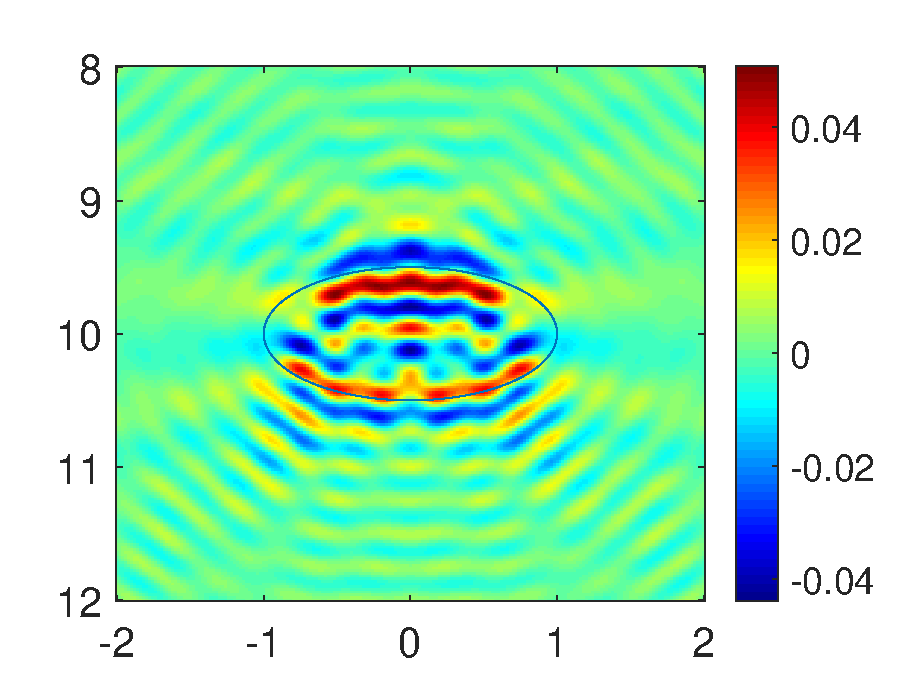
\includegraphics[width=0.23\textwidth]{./phaseless/ex1/ex1phaseless1}
  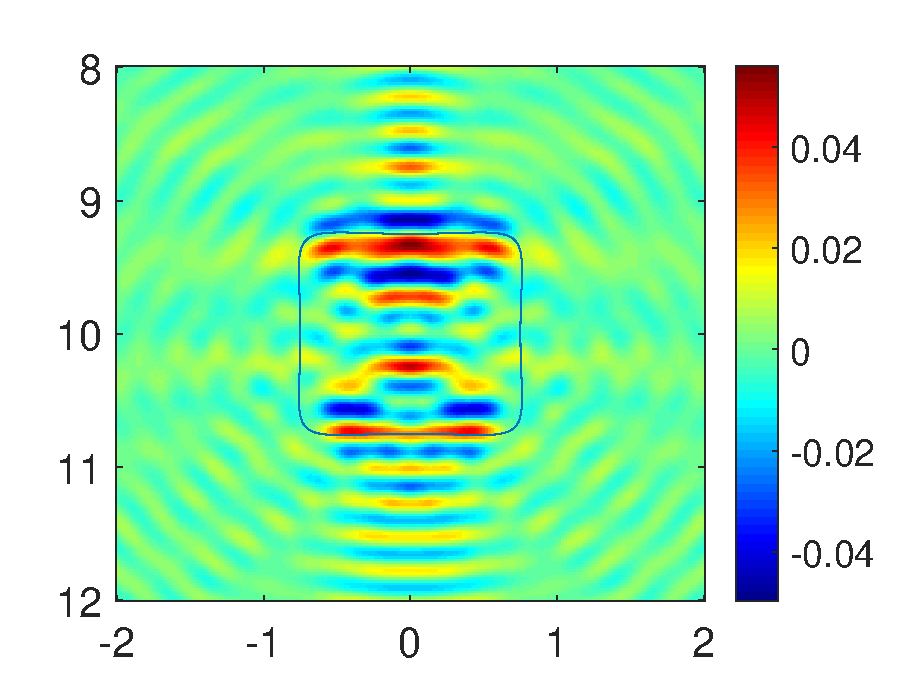
\includegraphics[width=0.23\textwidth]{./phaseless/ex1/ex1phaseless2}
  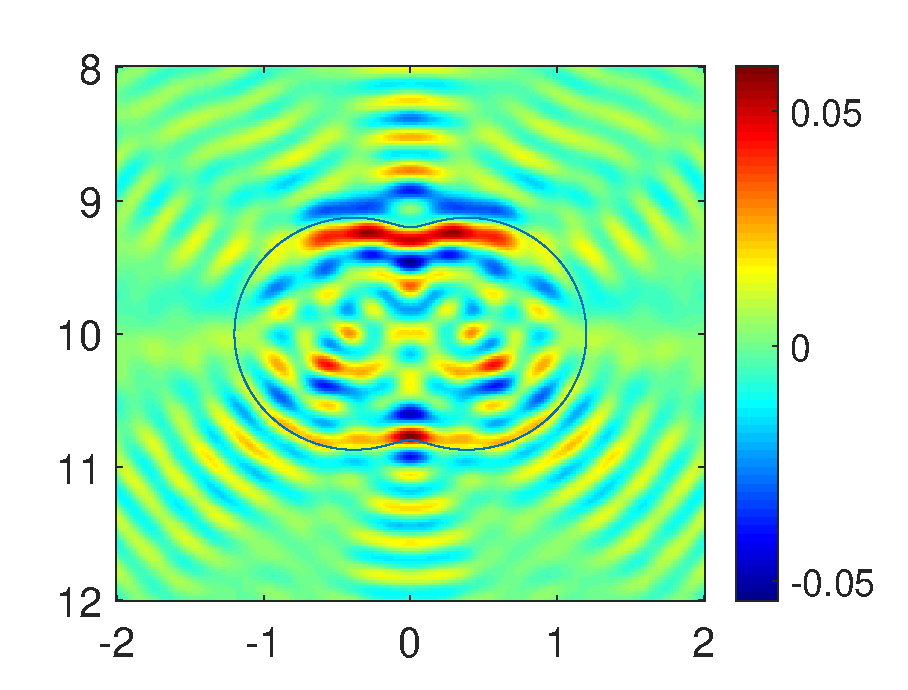
\includegraphics[width=0.23\textwidth]{./phaseless/ex1/ex1phaseless3}
  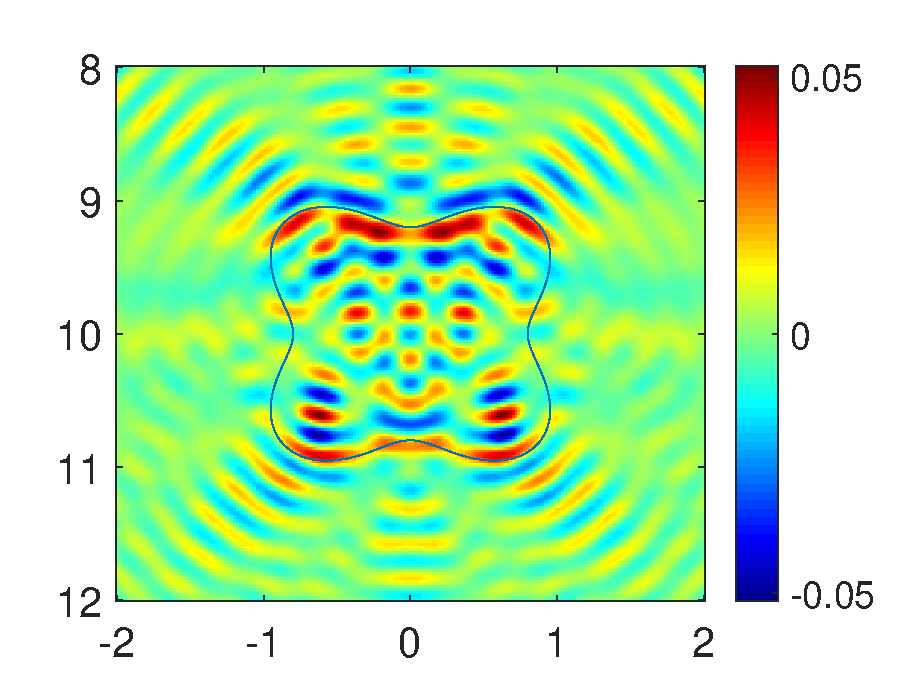
\includegraphics[width=0.23\textwidth]{./phaseless/ex1/ex1phaseless4}\\
  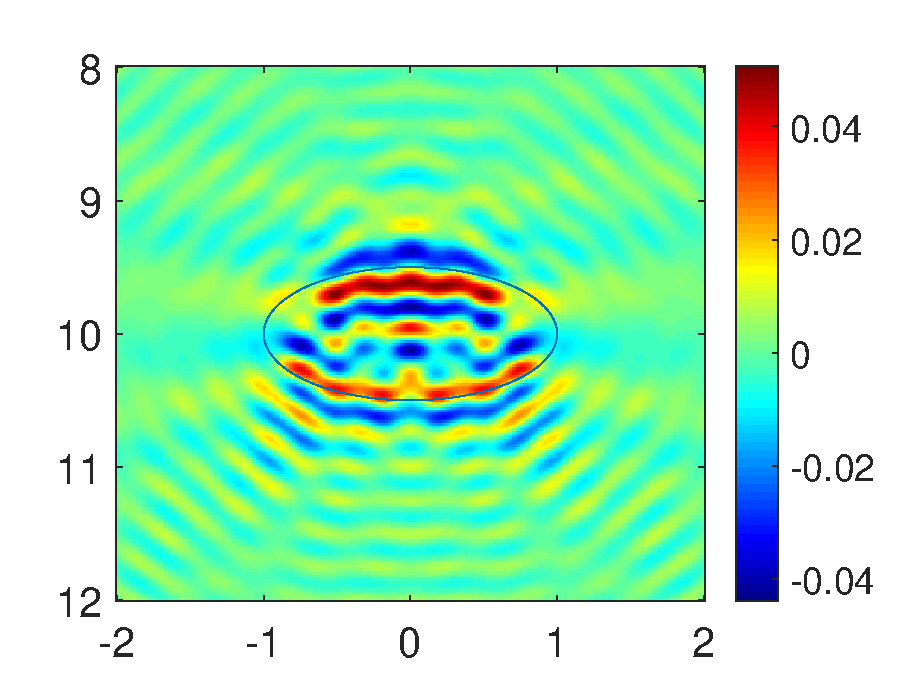
\includegraphics[width=0.23\textwidth]{./phaseless/ex1/ex1phase1}
  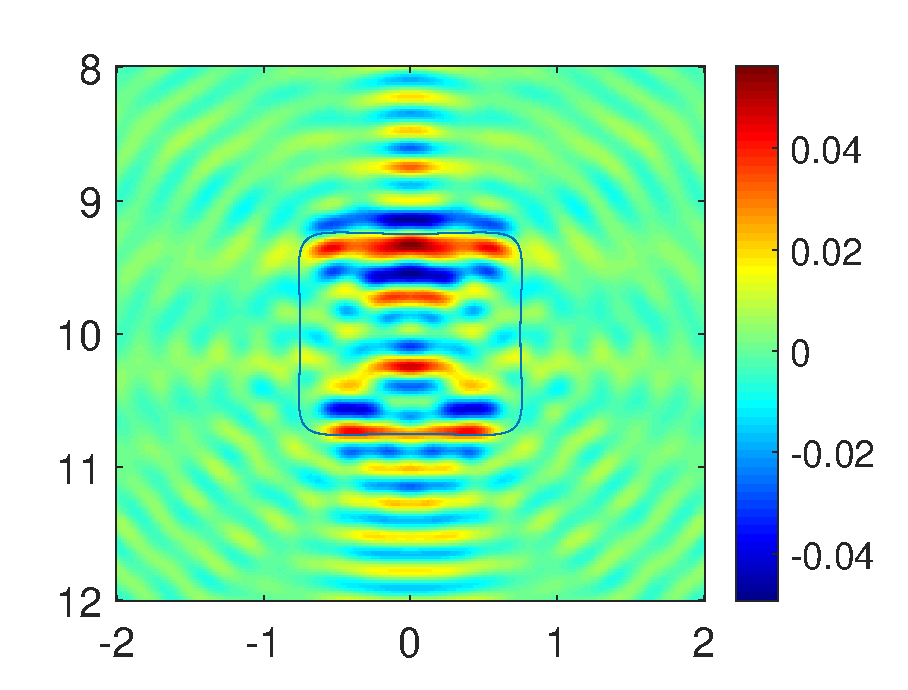
\includegraphics[width=0.23\textwidth]{./phaseless/ex1/ex1phase2}
  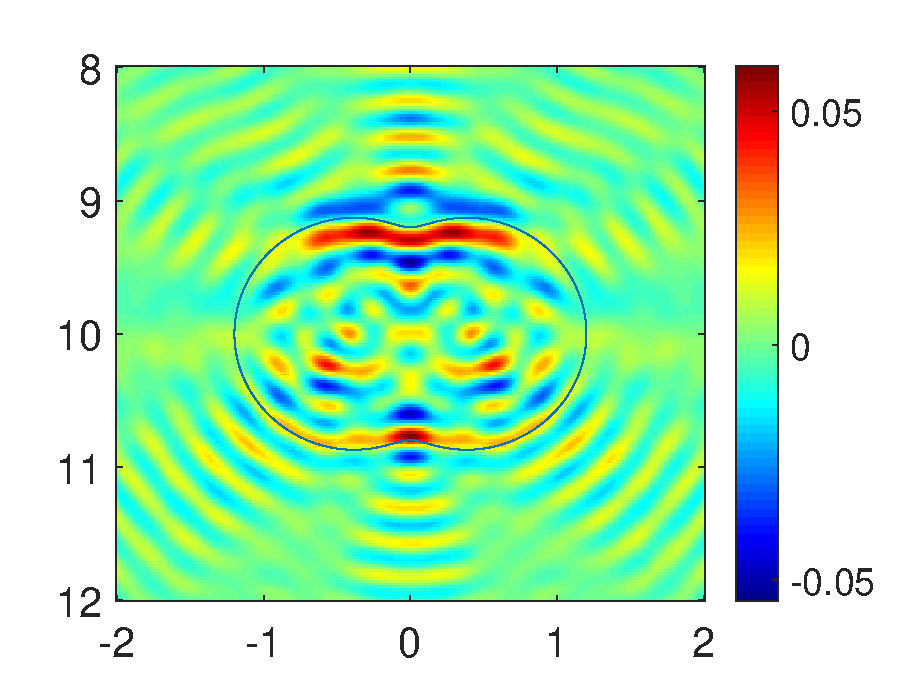
\includegraphics[width=0.23\textwidth]{./phaseless/ex1/ex1phase3}
  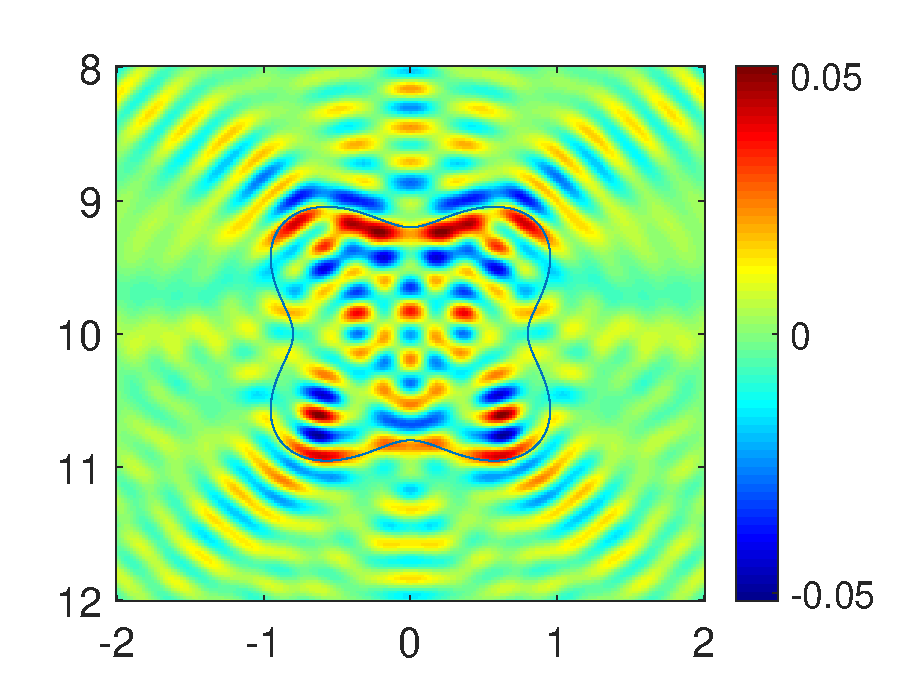
\includegraphics[width=0.23\textwidth]{./phaseless/ex1/ex1phase4}
  \caption{算例\ref{hp_ex1}:不同形状的可穿透障碍物,其中第一行为半空间无相位成像算法,第二行为半空间逆时偏移算法。参数为:$k=4\pi$, and $N_s=512$, $N_r=512$。} \label{fig1}
\end{figure}

\begin{example}\label{hp_ex2}
在本算例中,我们以具有椭圆形状的障碍物为例,考察新提出的半空间无相位逆时偏移算法对具有不同边界类型的障碍的成像效果,如声软障碍物,声硬障碍物以及阻尼系数为$\eta=1$的阻抗边界障碍物。采样区域为$\Omega=[-2,2]\times[8,12]$,且
我们使用$201\times201$的均匀采样。探测频率$k=4\pi$,源点和接收点个数为$N_s=512$, $N_r=512$。

图片 \ref{fig2}表明了仅仅使用总场的无相位数据,新算法也可以对各种边界类型的障碍物边界进行成像,确定其位置和形状。此外,我们强调一下,因为在$x_r\in\Gamma_0^d$接收到的数据并不包含障碍物下边界的信息,所以对不可穿透障碍物,仅能对障碍物上边界进行成像。
\end{example}
\begin{figure}[h]
  \centering
  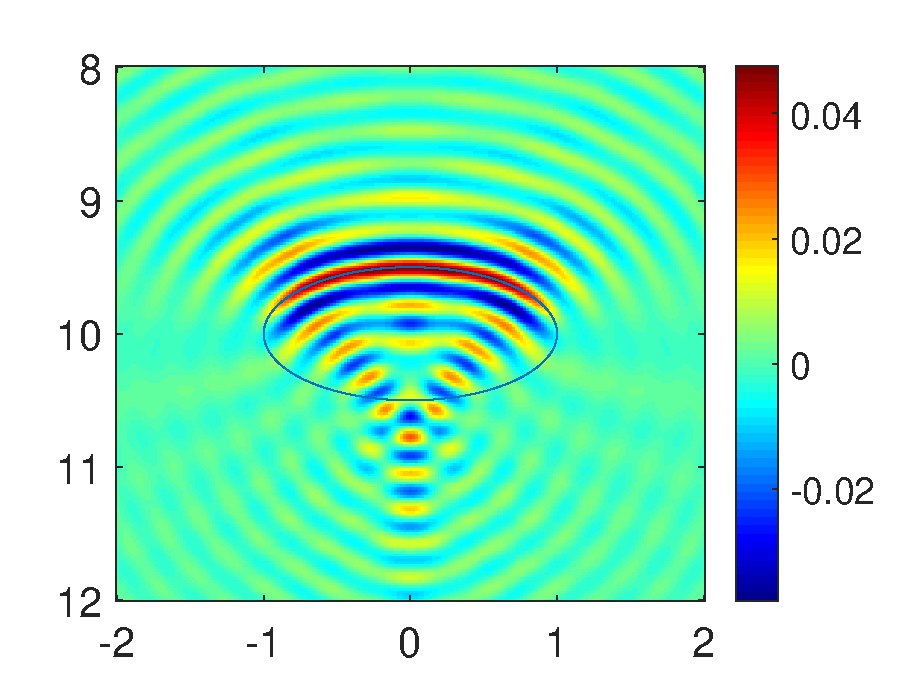
\includegraphics[width=0.3\textwidth]{./phaseless/ex2/ex2elliptic2}
  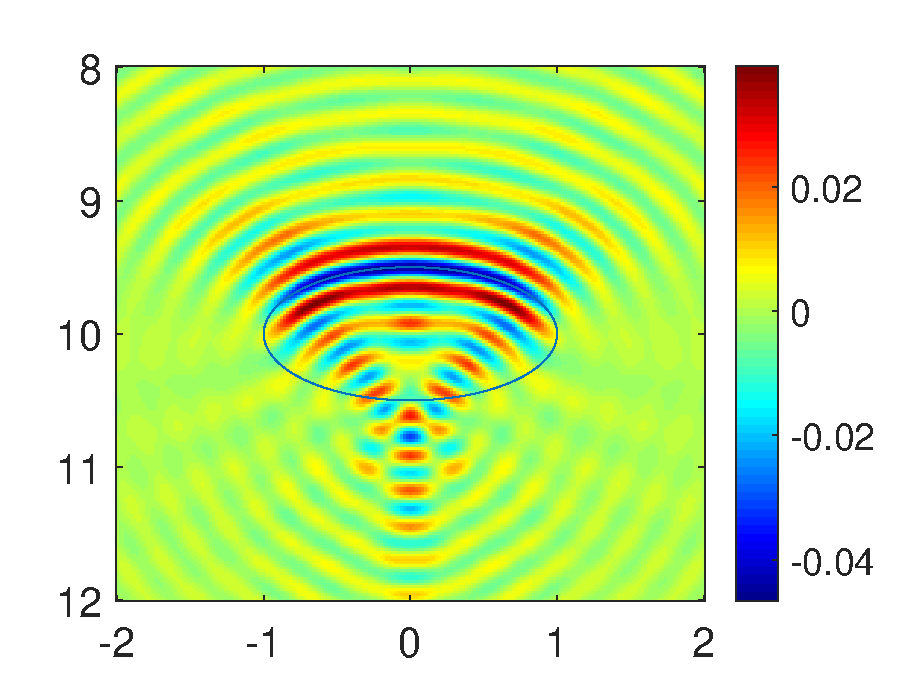
\includegraphics[width=0.3\textwidth]{./phaseless/ex2/ex2elliptic3}
  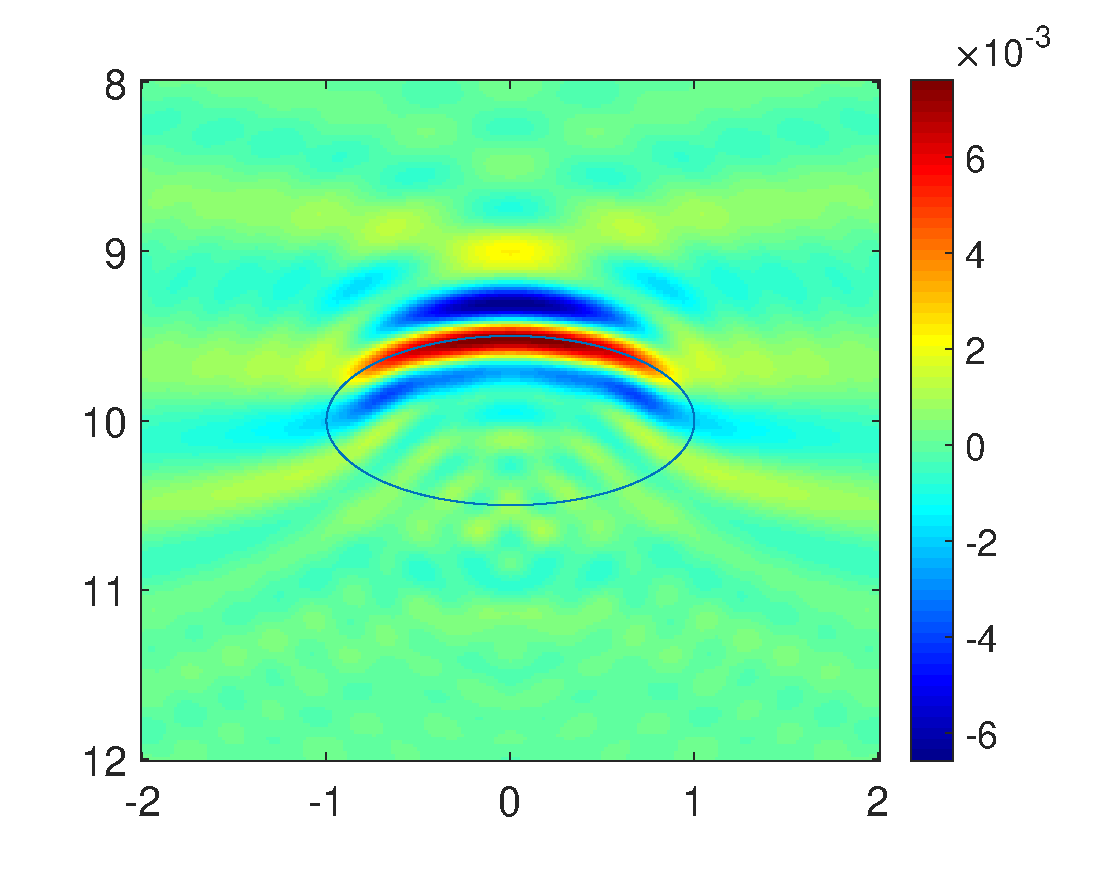
\includegraphics[width=0.3\textwidth]{./phaseless/ex2/ex2elliptic4}
    \caption{算例\ref{hp_ex2}:不同类型的椭圆型障碍物,从左到右依次为声软、声硬和阻抗系数为$\lambda\equiv1$的阻抗障碍物 。 参数为:$k=4\pi$, and $N_s=512$, $N_r=512$。}\label{fig2}
\end{figure}
\begin{example}\label{hp_ex3}
在本算例中,我们分别以单个频率和多个频率,来考察新提出的半空间无相位逆时偏移算法的抗干扰性。假设接受到的总场数据中带有如下形式的高斯噪音,
$$ |u|_{noise}=|u|+v_{noise},$$
其中
$$v_{noise}=\mu \max{|u|}\epsilon,\ \ and\ \ \epsilon\sim N(0,1).$$
采样区域为$\Omega=[-2,2]\times[8,12]$或者$\Omega=[-5,5]\times[6,16]$,且
我们使用$201\times201$的均匀采样。探测频率$k=4\pi$或$k=2\pi\times[1:0.25:3]$,源点和接收点个数为$N_s=256$, $N_r=256$。

在我们的第一个测试中,我们采用单个的可穿透障碍物作为成像目标,首先使用单频$k=2\pi$作为探测频率。图片 \ref{fig3}的第一行验证了当新算法使用带噪音的数据时,依然可以对障碍物进行有效成像,其中噪音水平依次为$\mu = 10\%, 20\%, 30\%, 40\%$。这就很好地验证了当噪音水平不断变大时,成像算法的稳定性。然后我们使用多频的数据来期望进一步提高成像效果,取频率为$k=2\pi\times[1:0.25:3]$。图片 \ref{fig3} 的第二行展示了相应噪音水平下多频的成像效果。可以看到,当采用多个频率时,噪音和振荡被抵消和压制,聚焦效果更加明显,极大地提升了成像效果。

在我们的第二个测试中,我们采用两个声软障碍物来作为成像目标,同样分别采用单频和多频以便加以对比。采样区域为$\Omega=[-5,5]\times[6,16]$,且我们使用$201\times201$的均匀采样。图片\ref{fig4}展示了不同噪音水平下,使用总场无相位数据时,新算法对多个障碍物的成像效果,同样我们观察到多频叠加的抗干扰能力和聚焦能力得到显著提高。在文献\cite{Robert2007Inverse}的定理4.1中,Robert Gilbert对Pekeris开波导模型下,证明了可穿透障碍物反散射问题的唯一性。
\end{example}

\begin{figure}[h]
  \centering
  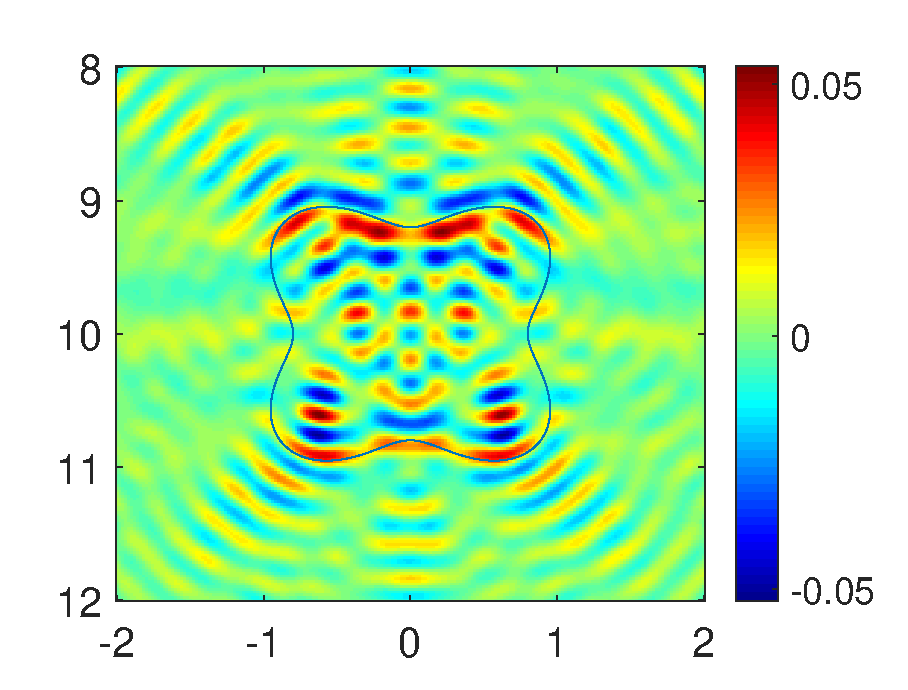
\includegraphics[width=0.23\textwidth]{./phaseless/ex3/ex3singlefreqsigma1}
  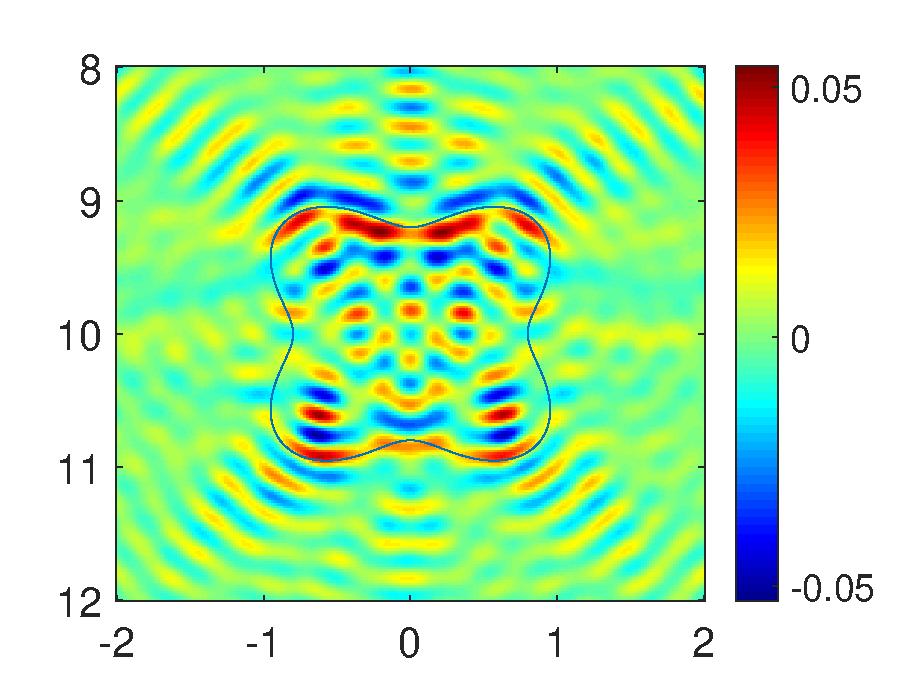
\includegraphics[width=0.23\textwidth]{./phaseless/ex3/ex3singlefreqsigma2}
  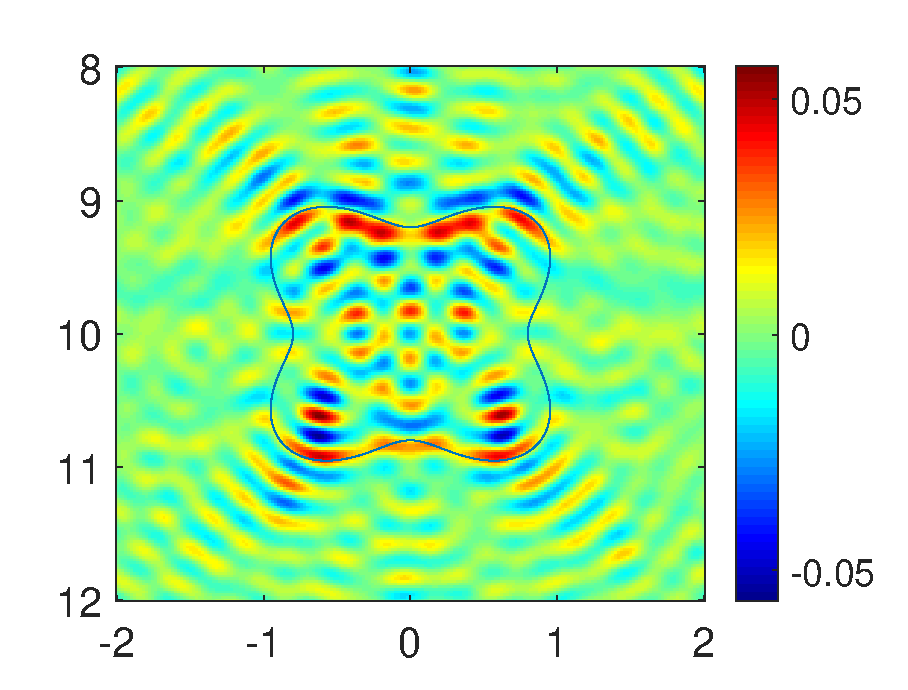
\includegraphics[width=0.23\textwidth]{./phaseless/ex3/ex3singlefreqsigma3}
  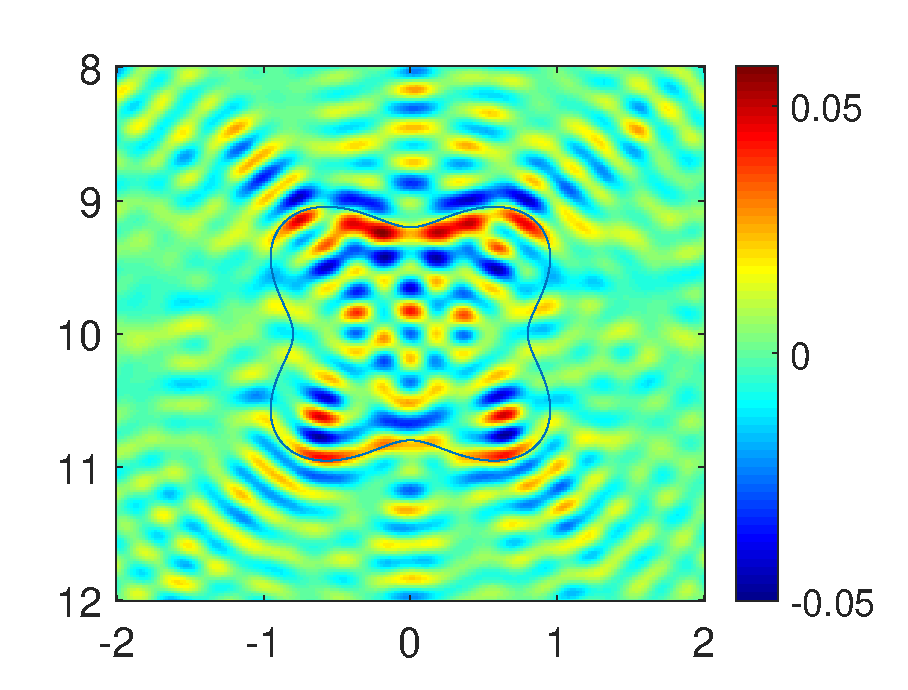
\includegraphics[width=0.23\textwidth]{./phaseless/ex3/ex3singlefreqsigma4}\\
  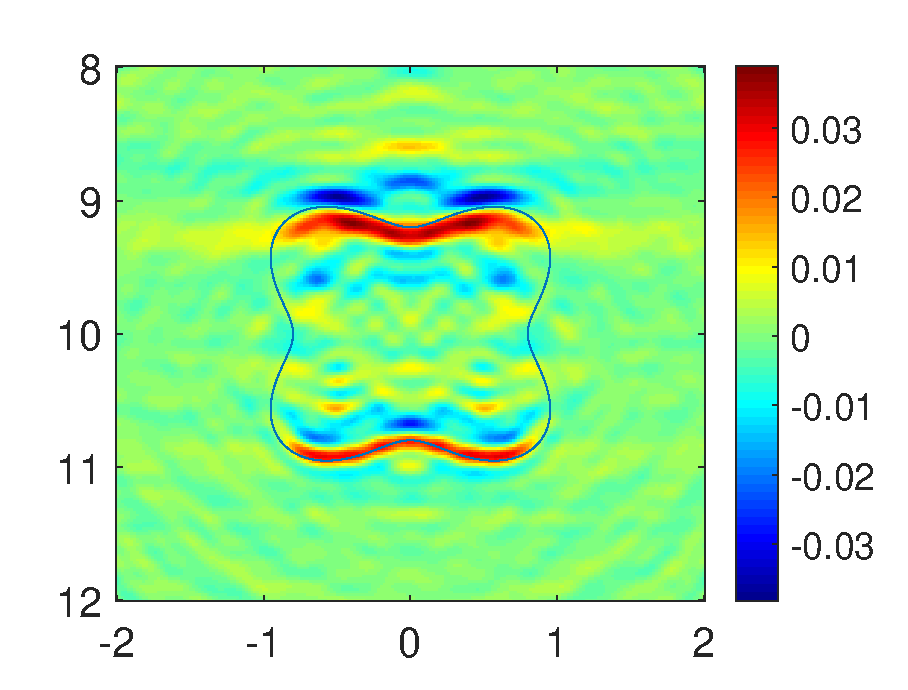
\includegraphics[width=0.23\textwidth]{./phaseless/ex3/ex3multifreqsigma1}
  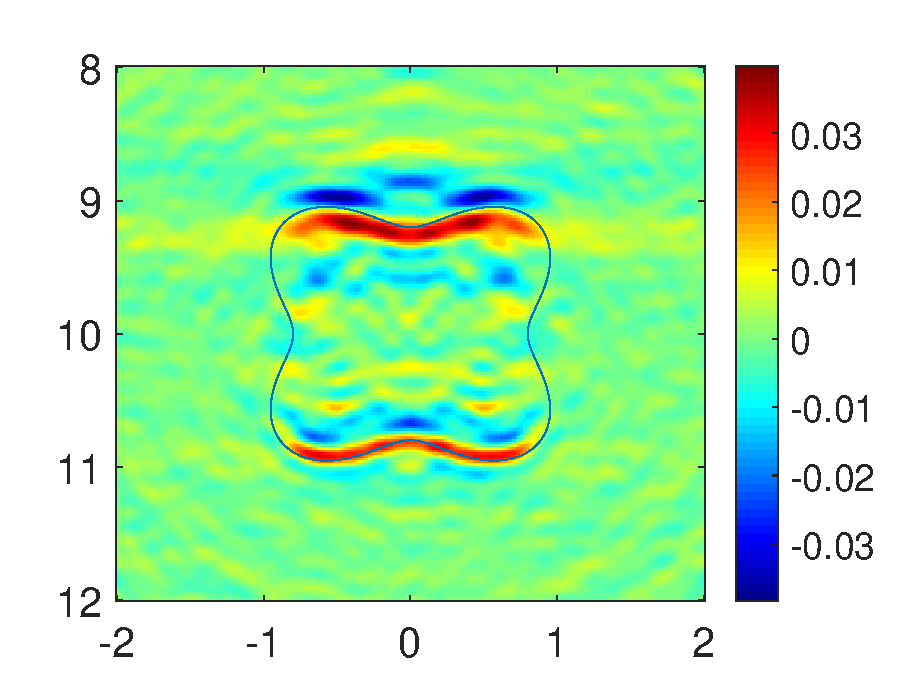
\includegraphics[width=0.23\textwidth]{./phaseless/ex3/ex3multifreqsigma2}
  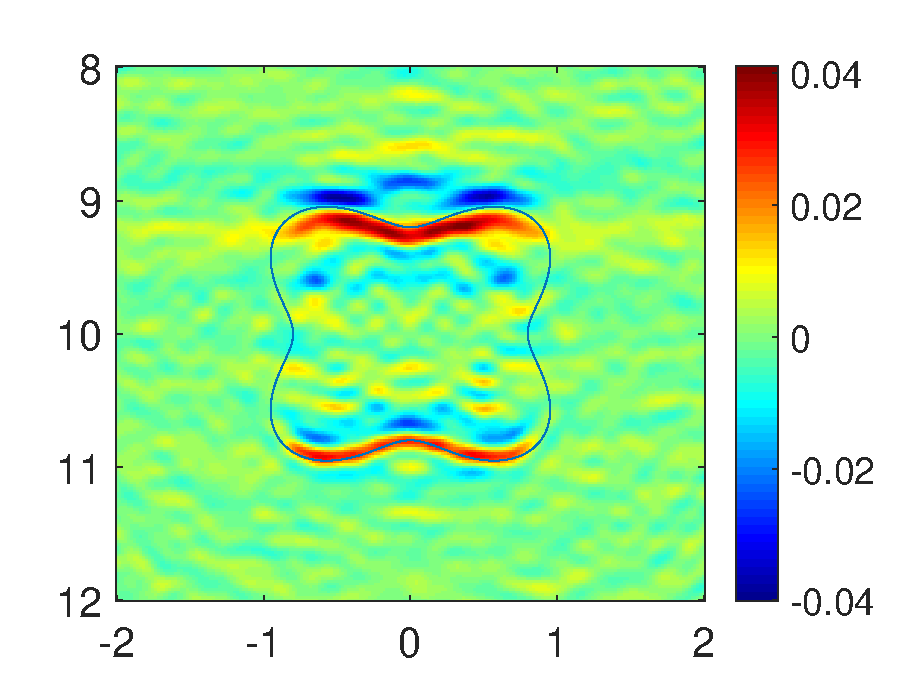
\includegraphics[width=0.23\textwidth]{./phaseless/ex3/ex3multifreqsigma3}
  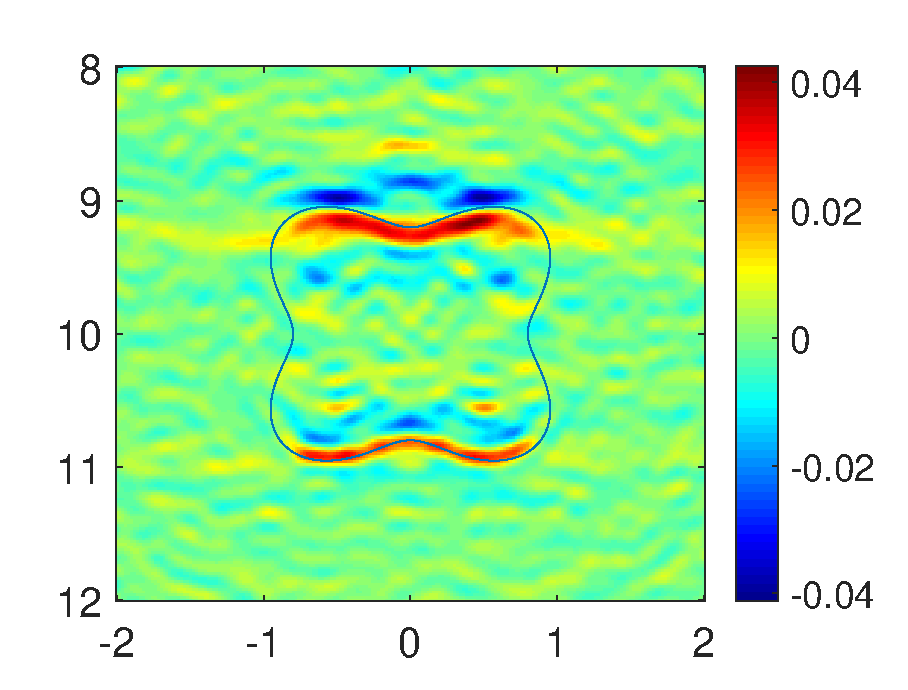
\includegraphics[width=0.23\textwidth]{./phaseless/ex3/ex3multifreqsigma4}
    \caption{算例\ref{hp_ex2}测试1: 带噪音数据的可穿透障碍物成像,噪音水平从左到右依次为为: $\mu=0.1,0.2,0.3,0.4$。
    第一行是单频测试结果,第二行为多频叠加结果。}\label{fig3}
\end{figure}
\begin{figure}[h]
  \centering
    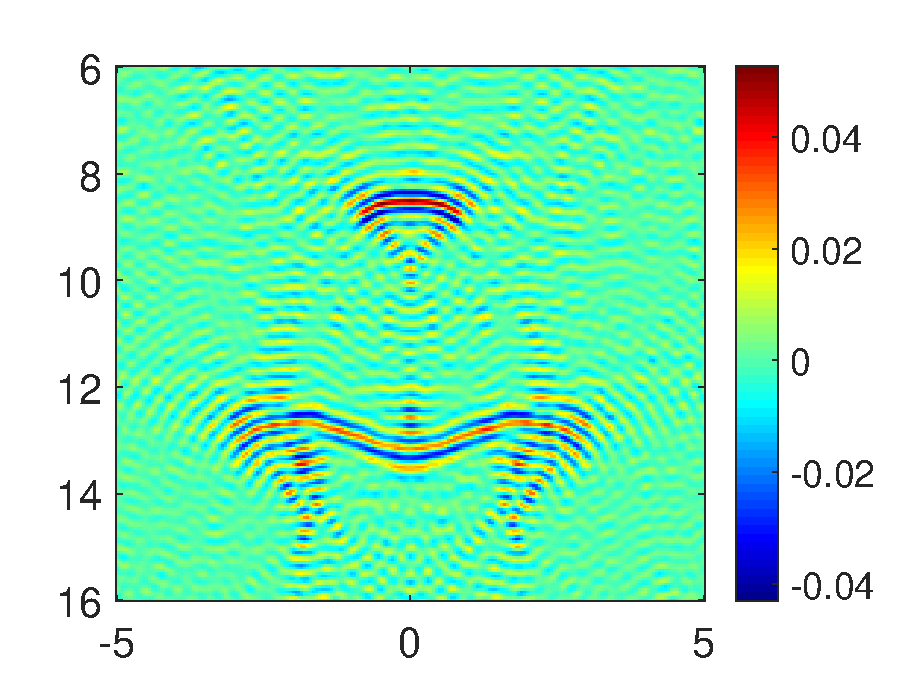
\includegraphics[width=0.23\textwidth]{./phaseless/ex4/ex4singlefreqsigma1}
  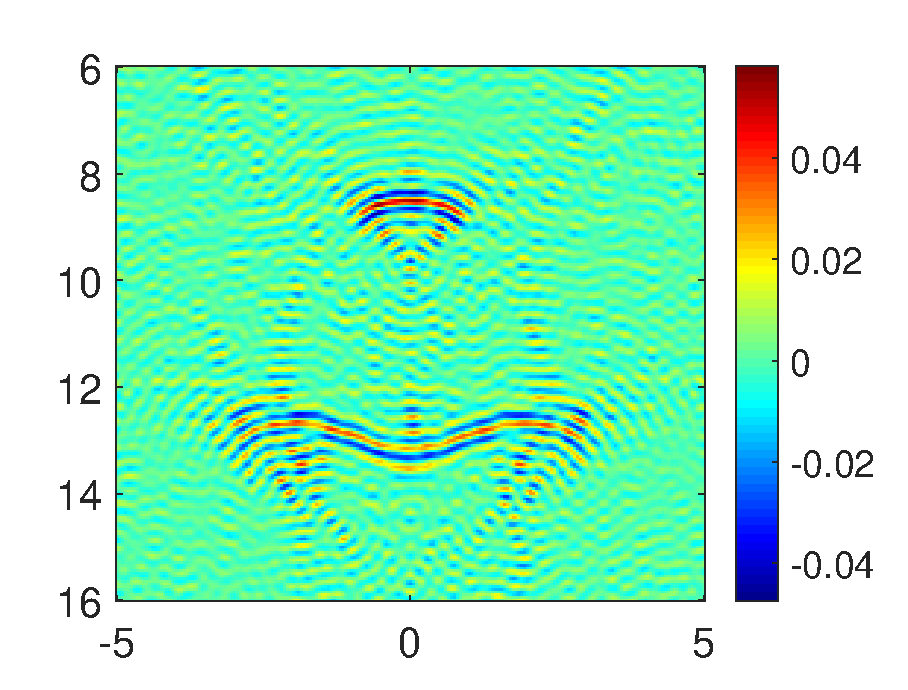
\includegraphics[width=0.23\textwidth]{./phaseless/ex4/ex4singlefreqsigma2}
  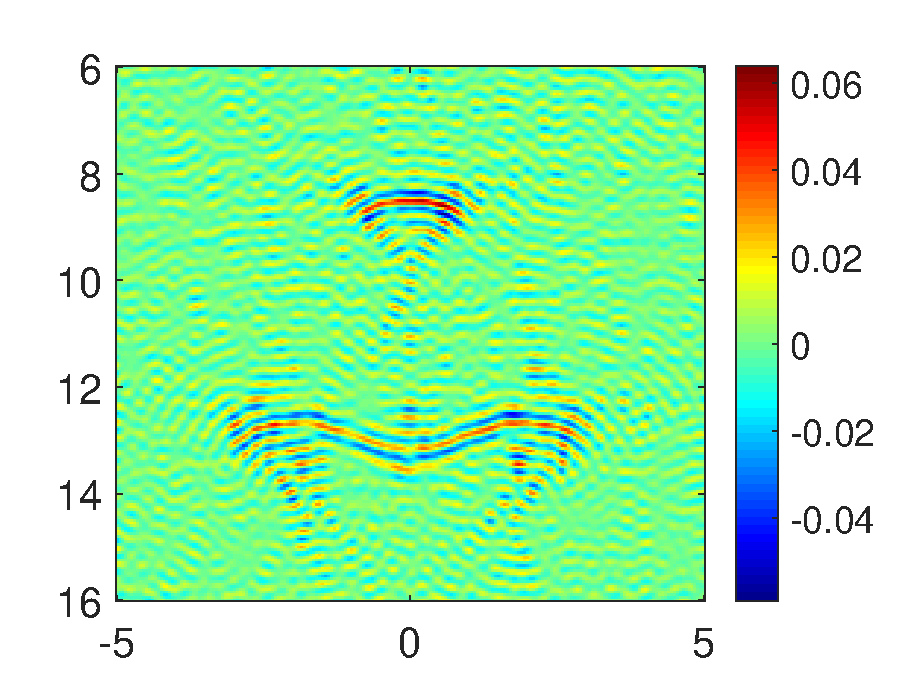
\includegraphics[width=0.23\textwidth]{./phaseless/ex4/ex4singlefreqsigma3}
  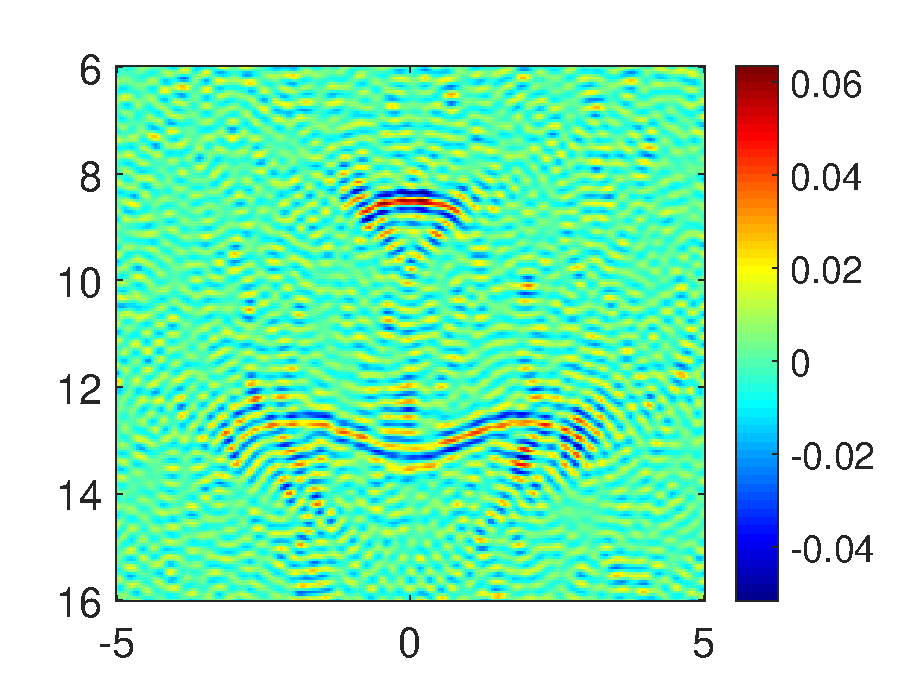
\includegraphics[width=0.23\textwidth]{./phaseless/ex4/ex4singlefreqsigma4}\\
      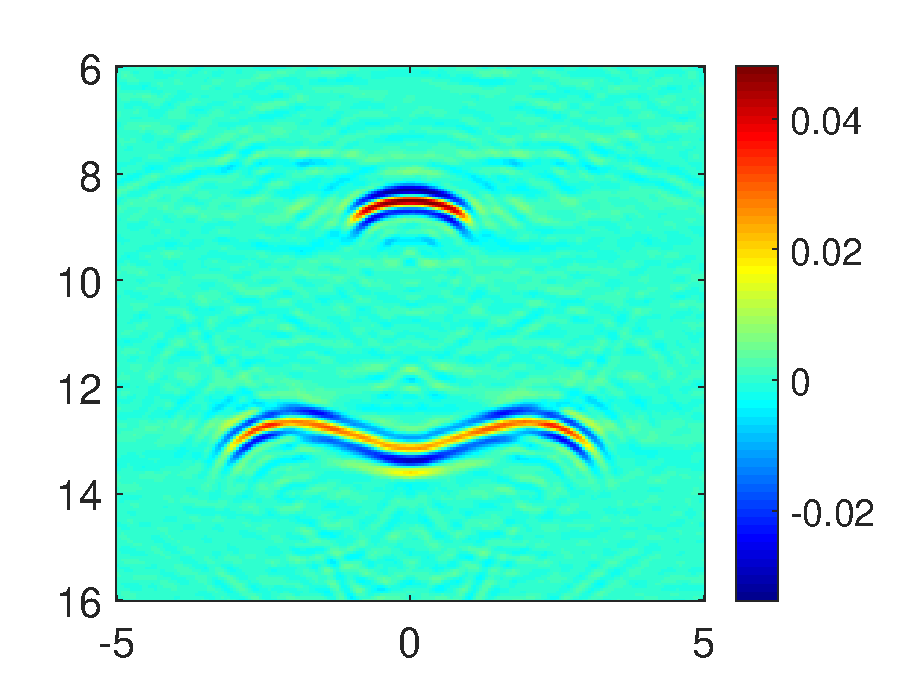
\includegraphics[width=0.23\textwidth]{./phaseless/ex4/ex4multifreqsigma1}
  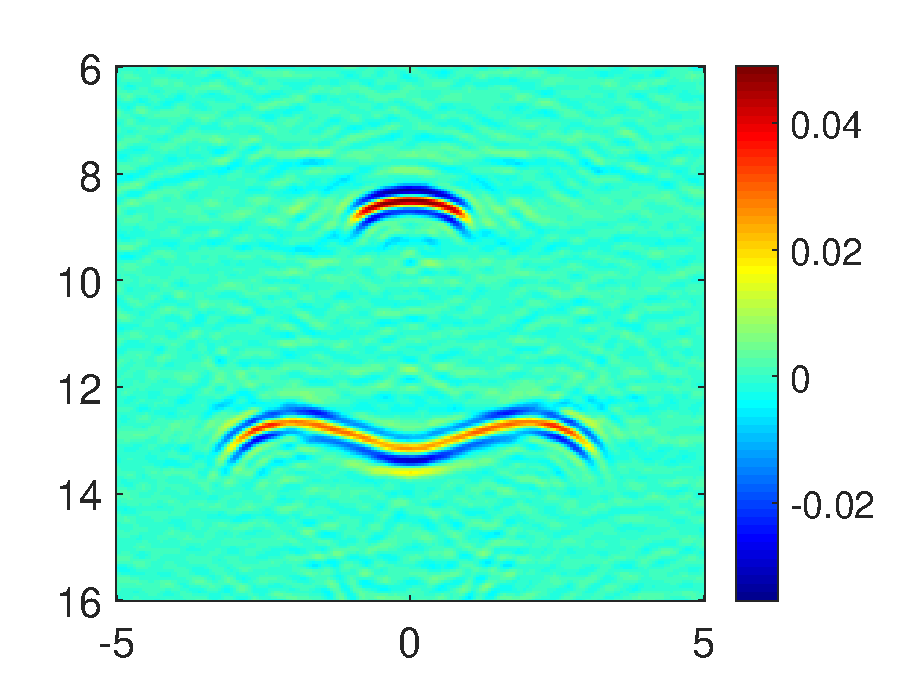
\includegraphics[width=0.23\textwidth]{./phaseless/ex4/ex4multifreqsigma2}
  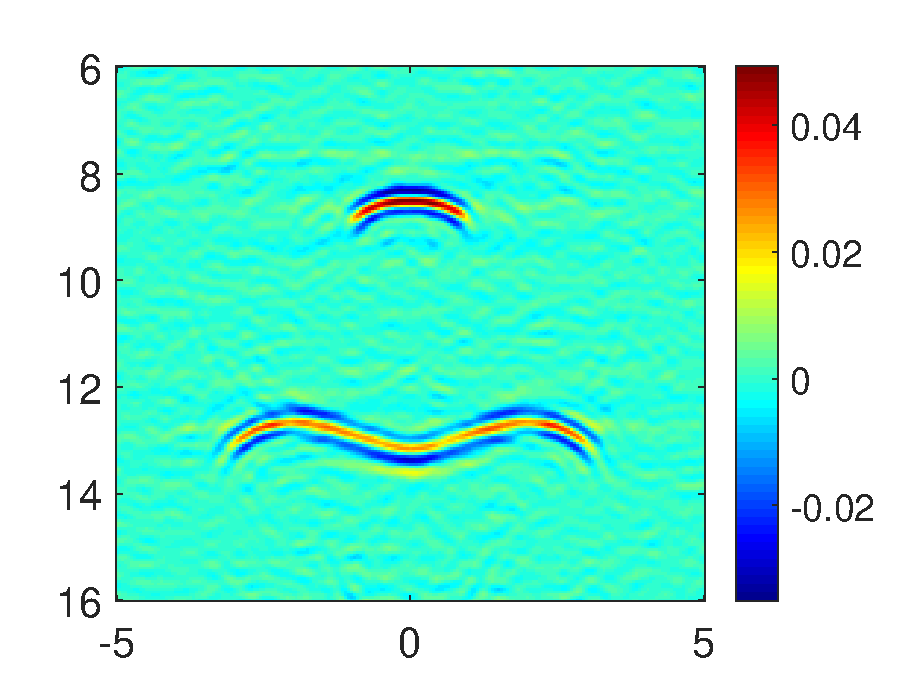
\includegraphics[width=0.23\textwidth]{./phaseless/ex4/ex4multifreqsigma3}
  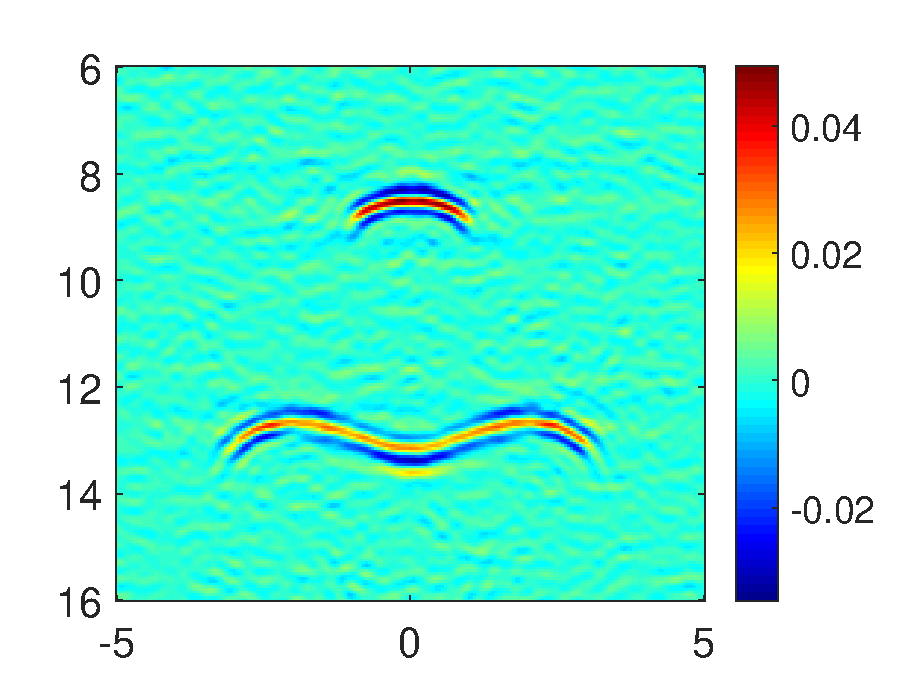
\includegraphics[width=0.23\textwidth]{./phaseless/ex4/ex4multifreqsigma4}
    \caption{算例\ref{hp_ex2}测试2: 带噪音数据的两个声软障碍物成像, 参数设置与\ref{fig3}完全一样。}\label{fig4}
\end{figure}
\begin{remark}
从上一节的数值测试结果可以看出,在障碍物$D$远离半空间边界$\Gamma_0$时,本章所提直接成像算法\ref{alg_phaseless}可以达到文献\cite{ch_ha}中所提半空间逆时偏移算法相同的分辨率。同样的,对于不可穿透障碍物,算法\ref{alg_phaseless}仅能够对障碍物$D$上半边界进行成像。这种现象在文献\cite{ch_ha}通过高频渐进分析和散射系数进行了说明,为了保证完整性,我们将在本文附录对Hemholtz散射系数加以补充和说明,此处不再详述。
\end{remark}
\section{本章小结}

在本章,我们主要考虑了声波半空间障碍物成像问题。特别地,我们提出了一种直接成像算法\ref{alg_phaseless}。该算法可以解决如下问题:

当在半空间边界$\Gamma_0:=\{(x_1,x_2)\in\R^2_+,x_1\in\R,x_2=0\}$上所采集的数据为无相位数据$u(x_r,x_s)$时,如何快速高效确定障碍物的位置、大小和形状?

除此之外,我们还对算法\ref{alg_phaseless}进行了分辨率分析,理论研究表明:当障碍物$D$远离半空间边界$\Gamma_0$时,算法\ref{alg_phaseless}可以达到文献\cite{ch_ha}中半空间逆时偏移算法相同的分辨率。数值测试表明算法\ref{alg_phaseless}还继承了半空间逆时偏移算法的优点:在不需要知道障碍物的任何信息的情况下,例如是否可穿透以及可穿透障碍物的边界条件,算法\ref{alg_phaseless}能够对不同类型不同形状的障碍物进行有效成像;并且算法的抗噪性能和多频测试结果也都令人十分满意。


\chapter{Pekeris开波导逆散射问题}

从本章开始,我们将研究Pekeris 开波导逆散射问题。在地质勘探、海洋成像以及光纤通信等领域,开波导模型具有非常重要的实际应用。
由于波导模式的存在,当障碍物嵌入在开波导模型当中时,如何确定其位置、大小和形状将变得极其复杂。

通过对点扩散函数的分析和数值测试,我们提出了求解开波导障碍物成像问题的单频逆时偏移算法。该算法能够对不同类型的障碍物进行有效成像,确定其位置、大小和形状,并且不需要提前知道障碍物的先验信息。特别地,当障碍物位于波导第一层时,成像效果类似于闭波导情形
\cite{ch_cw},障碍物的上下边界都能够有效成像;当障碍物位于波导第二层时,成像效果类似于一般半空间情形\cite{ch_ha},对于不可穿透障碍物仅能确定其上半边界。大量的数值算例验证了开波导逆时偏移算法对障碍物成像问题的有效性。

\section{问题介绍}
\begin{figure}[b]
  \centering
  % Requires \usepackage{graphicx}
  \caption{Pekeris模型}
  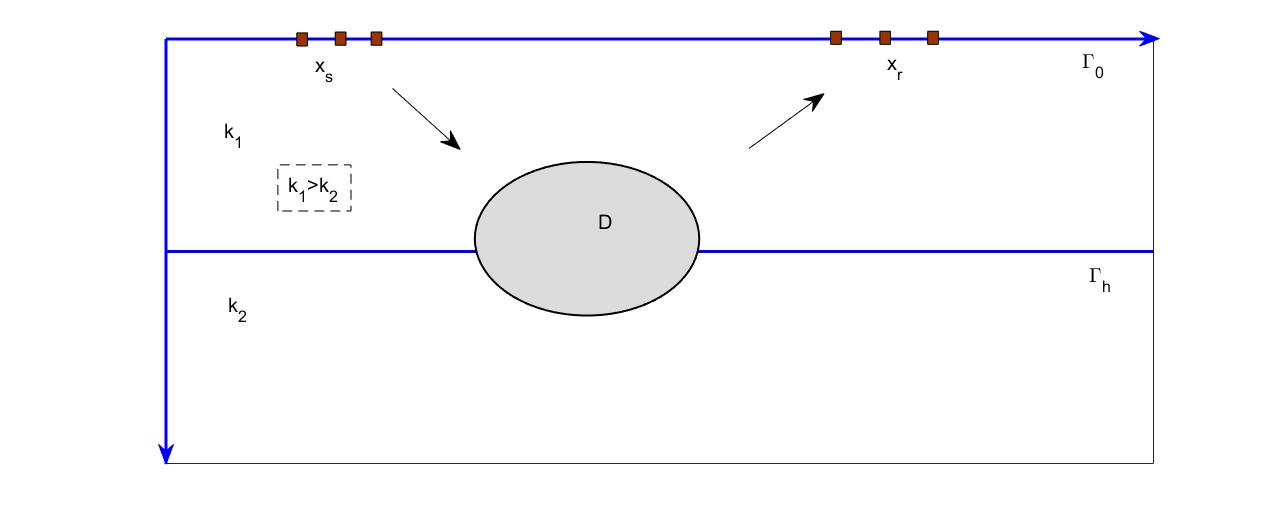
\includegraphics[width=14cm,height=5cm]{./pekeris/wg_forward}
\label{pekeris_model}
\end{figure}
如图\ref{pekeris_model} 所示,假设可穿透障碍物$D$嵌入在Pekeris模型当中,其中背景介质波数$k(x)$ 为
\begin{eqnarray}
k(x)=\left\{
\begin{array}{lll}
  k_1&,&x_2\in(0,h)\\
  k_2&,&x_2\in(h,+\infty)
\end{array}
\right.
\end{eqnarray}
其中$k_1>k_2$,并记$\Gamma_0,\Gamma_h,L_1,L_2$ 分别为

\begin{itemize}
  \item $ \Gamma_0=\{(x_1,x_2);x_1\in \R, x_2=0\}$;\quad\quad$ \Gamma_h=\{(x_1,x_2);x_1\in \R, x_2=h\}$
  \item $ L_1=\{(x_1,x_2);x_1\in \R, 0<x_2<h\}$;\quad\quad$ L_2=\{(x_1,x_2);x_1\in \R, x_2>h\}$
\end{itemize}


假设可穿透障碍物$D$是一个有界的Lipschitz区域。设源点$x_s\in\Gamma_0$,并记$u(x,x_s)$ 为由源点$x_s$ 激发产生的总场,其满足如下方程
\begin{eqnarray}\label{wg_totalfield}
\left\{
\begin{array}{lll}
 \Delta_x u(x,x_s)+k^2(x)n(x)u(x,x_s)=-\delta_{x_s}(x), &in& \R^2_+,\\
 & &\\
 \left[u(\cdot,x_s)\right]_{\Gamma_h}=\left[\frac{\partial u(\cdot,x_s)}{\partial\nu}\right]_{\Gamma_h}=0\\
 & &\\
 \frac{\partial u(x,x_s)}{\partial x_2(x)}=0,  &on& \Gamma_0.
 \end{array}
 \right.
\end{eqnarray}
其中函数$n(x)\in L^{\infty}(\R^2_+)$是一个处处大于零,且在$\R^2_+\backslash\overline D$ 上恒等于1的标量函数。
为保证散射问题\eqref{wg_totalfield}的适定性,我们还需要在无穷远处添加合适的辐射条件。

当背景为均匀介质时,传统的Sommerfeld辐射条件\eqref{Sommerfeld}保证了声波散射问题的唯一性和存在性,然而当背景为分层介质时,Sommerfeld辐射条件不再适用。通过对积分形式的Sommerfeld辐射条件加以推广,Ciraolo和Magnanini\cite{Ciraolo2009A1,Ciraolo2009A2}提出了适用于全空间三层开波导模型的Sommerfeld—Rellich型辐射条件,并在一定假设下证明了可穿透障碍物散射问题的存在性和唯一性。于此同时,Bonnet-Ben
Dhia和Christophe Hazard 等人\cite{Dhia2009DIFFRACTION} 基于广义的Fourier变换(Generalized Fourier Transform) 提出了模式辐射条件(Modal Radiation Condition),并且证明了Pekeris 开波导散射问题的存在性和唯一性。此外,关于辐射条件,还有Nedelec 在文献\cite{Jerez2012Asymptotics}中的讨论,其目的是为了研究开波导正散射问题的PML数值解法。

如何通过测量到的散射数据来确定散射体$D$的位置、大小和形状就是本章将要解决的问题。之前我们提到过,针对类似的问题,Robert Gilbert\cite{Robert2007Inverse} 和Gang Bao\cite{Bao2013Reconstruction} 对唯一性进行了研究;Habib Ammari\cite{Ammari2005Reconstruction} 提出了MUSIC型算法,当障碍物尺寸比较小时(Small inclusion assumpton),MUSIC 算法可以确定障碍物位置。Josselin Garnier\cite{Garnier2012Correlation} 将Array Imaging 成像方法推广到了开波导情形,但是需要用到Born近似假设。

针对闭波导模型,文献\cite{ch_cw}提出了闭波导逆散射问题的逆时偏移算法,并建立严格了分辨率分析理论。类似于全空间逆散射问题的逆时偏移算法
\cite{cch_a,cch_e,ch_e},文献
\cite{ch_cw} 中的算法是基于(广义)Hemholtz-Kirchhoff恒等式而建立的,然而该恒等式在开波导情形不再成立,甚至在一般的声波半空间情形
\cite{ch_ha} 也不再成立。文献\cite{ch_ha} 针对声波半空间逆散射问题提出的逆时偏移算法是基于其所定义的点扩散函数的性质,通过对点扩散函数的分析建立起成像函数的分辨率分析。故而本章将以点扩散函数为出发点来构建我们的算法。

%本章剩余部分安排如下:
\section{Pekeris开波导正散射问题}
设源点$y\in\R^2_+$,引入Pekeris开波导Neumann零边界格林函数$N(x,y)$,其满足如下方程,
\begin{eqnarray}\label{G_Neumann}
\left\{
\begin{array}{lll}
  \Delta_xN(x,y)+k^2(x)N(x,y)=-\delta_y(x),&in&\R^2_+\\
  & &\\
  \left[N(\cdot,y)\right]_{\Gamma_h}=0,\ \ \left[\frac{\partial N(\cdot,y)}{\partial\nu}\right]_{\Gamma_h}=0 & &\\
  & &\\
  \frac{\partial N(x,y)}{\partial x_2}=0, &on&\Gamma_0
\end{array}
\right.
\end{eqnarray}
其中$\left[N(\cdot,y)\right]_{\Gamma_h}=0$,和$\left[\frac{\partial N(\cdot,y)}{\partial\nu}\right]_{\Gamma_h}=0$ 表示在界面$\Gamma_h$ 处的连续性条件。记$N_y(x_1,x_2):=N(x,y)$,并令$\hat{N}_y(\xi,x_2)$ 为$N_y(x_1,x_2)$关于变量$x_1$的Fourier变换:
\begin{equation}
\hat{N}_y(\xi,x_2)=\int^{\infty}_{-\infty}N_y(x_1,x_2)e^{-\i(x_1-y_1)\xi}dx_1
\end{equation}
利用$N(x,y)$为方程的外行波解,直接计算可得下述引理:
\begin{lemma}\label{FT_Neumann}
令$\xi=\xi_1+\i\xi_2,\xi_1,\xi_2\in\R$,以及$\mu_j=\sqrt{k_j^2-\xi^2},j=1,2$,并记关于$\xi$的函数$\hat N_h(\xi)$ 和$\hat M_h(\xi)$ 如下所示
\begin{eqnarray}\label{NhMh_N}
 \hat N_h(\xi)=\frac{\mu_1+\mu_2}{\mu_1-\mu_2}-e^{2\i\mu_1h},\ \
 \hat M_h(\xi)=\frac{\mu_1+\mu_2}{\mu_1-\mu_2}e^{2\i\mu_1h}-1
\end{eqnarray}
则当源点$y\in L_1$时,
\begin{eqnarray*}
\hat{N}_y(\xi,x_2)=\left\{
\begin{array}{lll}
\frac{\i}{2\mu_1}\left[e^{\i\mu_1|x_2-y_2|}+e^{\i\mu_1(x_2+y_2)}+
\frac{e^{2\i\mu_1h}\left[4\cos{(\mu_1x_2)\cos{(\mu_1y_2)}}\right]}{\hat N_h(\xi)}\right]&,&x_2\in(0,h)\\
& &\\
\frac{\i}{(\mu_1-\mu_2)\hat N_h(\xi)}\left[e^{\i\mu_2(x_2-h)+\i\mu_1(h-y_2)}
  +e^{\i\mu_2(x_2-h)+\i\mu_1(h+y_2)}\right]&,&x_2\in(h,+\infty)
\end{array}
\right.
\end{eqnarray*}
当源点$y\in L_2$时,
\begin{eqnarray*}
\hat{N}_y(\xi,x_2)=\left\{
\begin{array}{lll}
\frac{\i}{(\mu_1-\mu_2)\hat N_h(\xi)}\left[e^{\i\mu_1(h-x_2)+\i\mu_2(y_2-h)}+e^{\i\mu_1(x_2+h)+\i\mu_2(y_2-h)}\right]&,& x_2\in(0,h)\\
& &\\
\frac{\i}{2\mu_2}e^{\i\mu_2|x_2-y_2|}+\frac{\i}{2\mu_2}\frac{\hat M_h(\xi)}{\hat N_h(\xi)}e^{\i\mu_2(x_2+y_2-2h)}&,&  x_2\in(h,+\infty)
\end{array}
\right.
\end{eqnarray*}
\end{lemma}
\begin{remark}
由于上述引理中出现了$\mu_j,j=1,2$,我们假设对于任意地$z\in \mathbb{C}\backslash\{0\}$, $z^{1/2}$是$\sqrt{z}$ 的如下解析分支:$\Im(z^{1/2})\geq 0$,这对应于在复平面取右半实轴为割支线。则对于$z=z_1+\mathbf{i}z_2$, $z_1,z_2\in\R$,
\begin{equation}\label{branch}
  z^{1/2}=sgn(z_2)\sqrt{\frac{|z|+z_1}{2}}+\mathbf{i}\sqrt{\frac{|z|-z_1}{2}}
\end{equation}
当$z$位于右半实轴时,取$z^{1/2}$为$\epsilon\rightarrow0^+$ 时$(z+\i\epsilon)^{1/2}$ 的极限即可。
\end{remark}
\begin{remark}\label{Zeros_Neumann}
很明显,$\hat{N}_y(\xi,x_2)$的极点为函数$\hat N_h(\xi)$ 的零点。函数$\hat N_h(\xi)=0$等价于
\begin{equation}
  \mu_1+\mu_2+(\mu_2-\mu_1)e^{2\i\mu_1h}=0
\end{equation}
直接验证可知,当$\xi\in\{\xi\in\R;|\xi|\geq k_1,|\xi|<k_2\}$时,
$\hat N_h(\xi)\neq0$。于是当$\xi\in\R$时,$\hat N_h(\xi)$ 的零点仅仅分布在区间$[k_2,k_1)$,或区间$(-k_1,-k_2]$ 上。当$\xi=\pm k_2$ 时,我们有
\begin{equation}\label{cutoff}
  \hat N_h(\xi)=0\ \ \Rightarrow\ \ \sin\left(\sqrt{k_1^2-k_2^2}h\right)=0
\end{equation}
若记$\omega$表示频率,$c_1,c_2$分别为开波导第一、二层的背景介质速度,则$k_j=\frac{\omega}{c_j}$。 求解方程\eqref{cutoff}可得频率
\begin{equation}
\omega=\frac{c_1c_2}{\sqrt{c_1^2-c_2^2}}\frac{n\pi}{h},\ \ n\in\mathbb{Z}
\end{equation}
这些解被称为截断频率,关于截断频率的更多讨论可见文献\cite{Katsnelson2012Fundamentals,Kuperman2011Computational}。 本文我们假设$\sin\left(\sqrt{k_1^2-k_2^2}h\right)\neq0$ 以保证模型不会产生截断频率,从而$\pm k_2$ 不再是$\hat N_h(\xi)$ 的零点。
最后当$\xi\in(k_2,k_1)$ 时,$\hat N_h(\xi)=0$等价于
\begin{equation}
  \tan{\left(\sqrt{k_1^2-\xi^2}h\right)}=\frac{\sqrt{\xi^2-k_2^2}}{\sqrt{k_1^2-\xi^2}}
\end{equation}
记$\hat N_h(\xi)$在区间$(k_2,k_1)$上的零点个数为$\hat M$, 则由上式可知,
$\hat M\leq\left[\sqrt{k_1^2-k_2^2}h/\pi\right]+1$。 我们记这$\hat M$个零点为$\hat\xi_1,\ldots,\hat\xi_{\hat M}$,易验证$\hat N'_h(\hat\xi_m)\neq0$,于是这$\hat M$个零点都是$\hat N_h(\xi)$ 的一阶零点,它们对应了Pekeris 开波导模型的$\hat M$ 个波导模式。
\end{remark}
由注\ref{Zeros_Neumann} 可知,函数$\hat N_y(\xi,x_2)$在实轴上存在一阶奇点,故而直接在实轴上对其进行逆Fourier变换是行不通的。为解决这一困难,我们可以参考文献\cite{cz2010,Chew1995Waves,Desanto1992Scalar,thesis_guanghui} 中的做法,利用极限吸收原理并结合Cauchy积分定理,在Sommerfeld积分路径上进行逆Fourier变换,如图\ref{SIP_IFT}所示。关于SIP积分路径更多的讨论,有兴趣的读者可以文献\cite{Chew1995Waves}中的第二章。
\begin{figure}[htbp]
  \centering
  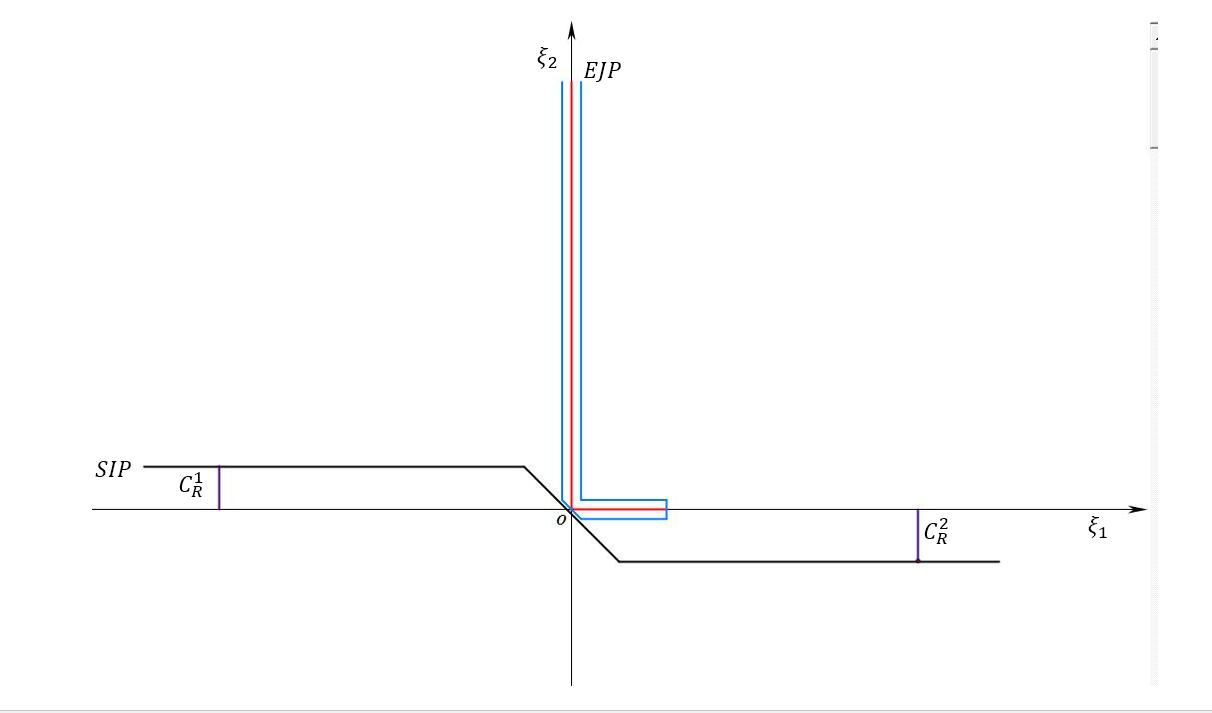
\includegraphics[width=15cm,height=6cm]{./SIP/SIP_IFT.jpg}
  \caption{Sommerfeld积分路径(SIP)}\label{SIP_IFT}
\end{figure}
在SIP上计算逆Fourier变换,我们就可以得到函数$N(x,y)$的积分表达式:
\begin{lemma}\label{f_Neumann}
令$\xi=\xi_1+\i\xi_2,\xi_1,\xi_2\in\R$,以及$\mu_j=\sqrt{k_j^2-\xi^2},j=1,2$,并记关于$\xi$的函数$\hat N_h(\xi)$ 和$\hat M_h(\xi)$ 如引理\ref{FT_Neumann}中所示,
则方程\eqref{G_Neumann} 所定义的函数$N(x,y)$有如下表达式
\begin{eqnarray*}
 N(x,y)=\left\{
 \begin{array}{lll}
   \Phi_{k_1}(x,y)+\Phi_{k_1}(x,y')+\hat S_1(x,y)&,&x\in L_1,y\in L_1\\
   \hat S_2(x,y)&,&x\in L_2,y\in L_1\\
   \hat K_1(x,y)&,&x\in L_1,y\in L_2\\
   \Phi_{k_2}(x,y)+\hat K_2(x,y)&,&x\in L_2,y\in L_2
 \end{array}
 \right.
\end{eqnarray*}
其中$\hat S_j(x,y), \hat K_j(x,y)$的表达式为
\begin{eqnarray*}
\left\{
\begin{array}{lll}
 \hat{S}_1(x,y)&=&\frac{1}{2\pi}\int_{SIP}\frac{\i}{2\mu_1}\frac{e^{2\i\mu_1h}
 \left[4\cos{(\mu_1x_2)\cos{(\mu_1y_2)}}\right]}{\hat N_h(\xi)}
  e^{\i(x_1-y_1)\xi}d\xi\\
  & &\\
 \hat{S}_2(x,y)&=&\frac{1}{2\pi}\int_{SIP}\frac{2\i e^{\i\mu_1h}\cos{(\mu_1y_2)}}{(\mu_1-\mu_2)\hat N_h(\xi)}e^{\i\mu_2(x_2-h)+\i(x_1-y_1)\xi}d\xi\\
 & &\\
 \hat{K}_1(x,y)&=&\frac{1}{2\pi}\int_{SIP}\frac{2\i e^{\i\mu_1h}\cos(\mu_1x_2)}{\hat N_h(\xi)}e^{\i\mu_2(y_2-h)+\i(x_1-y_1)\xi}d\xi\\
 & &\\
 \hat{K}_2(x,y)&=&\frac{1}{2\pi}\int_{SIP}\frac{\i}{2\mu_2}\frac{\hat M_h(\xi)}{\hat N_h(\xi)}e^{\i\mu_2(x_2+y_2-2h)+\i(x_1-y_1)\xi}d\xi
\end{array}
\right.
\end{eqnarray*}
\end{lemma}
然后通过留数定理,可以证明Pekeris开波导格林函数$N(x,y)$有如下的波导模式展开表达式:
\begin{lemma}[关于$N(x,y)$的波导模式展开]\label{Neumann_Mode}
设$\hat\xi_m$, $m=1,\ldots,\hat M$是$\hat N_h(\xi)$在区间$(k_2,k_1)$上的$\hat M$ 个实根,并记$\hat\mu_{1m}=\mu_1(\hat\xi_m),\hat\mu_{2m}=\mu_2(\hat\xi_m)$,则$N(x,y)$ 的波导模式展开为
\begin{equation*}
  N(x,y)=N_g(x,y)+N_{rad}(x,y)
\end{equation*}
其中$N_g(x,y)=\sum\limits_{m=1}^{\hat M} N_m(x,y)$,且
\begin{eqnarray}
\left\{
\begin{array}{lll}
  N_m(x,y)&=&\frac{\hat\mu_{2m}}{\hat\xi_m(1-\i\hat\mu_{2m}h)}\hat g(x_2,\hat\xi_m)\hat g(y_2,\hat\xi_m)e^{\i|x_1-y_1|\hat\xi_m}\\
  & &\\
 N_{rad}(x,y)&=&\frac{\i}{\pi}\int_{\i\infty}^{k_2}\frac{\mu_2 \hat g(x_2,\xi)\hat g(y_2,\xi)}{(k_1^2-k_2^2)\sin^2(\mu_1h)+\mu_2^2}e^{\ii|x_1-y_1|\xi}d\xi
\end{array}
\right.
\end{eqnarray}
其中$N_m(x,y)$中对应于$\hat\xi_m\in(k_2,k_1)$ 的函数$\hat g(x_2,\hat\xi_m)$表达式如下
\begin{eqnarray*}
\hat g(x_2,\hat\xi_m):=\left\{
 \begin{array}{lll}
   \cos(\hat\mu_{1m}x_2),& &x_2\in(0,h)\\
   & &\\
   \cos(\hat\mu_{1m}h)e^{\i\hat\mu_{2m}(x_2-h)},& &x_2\in(h,+\infty)
 \end{array}
 \right.
\end{eqnarray*}
此外,$N_{rad}(x,y)$中有向区间$[\i\infty,k_2]:=\{\xi;\xi\in[0,k_2],\ \ \mbox{或}\xi=\i\eta$,$\eta\in(0,+\infty)\}$,以及对应于$\xi\in[\i\infty,k_2]$的
函数$\hat g(x_2,\xi)$如下所示
 \begin{eqnarray*}
\hat g(x_2,\xi):=\left\{
 \begin{array}{lll}
   \cos(\mu_1x_2),& &x_2\in(0,h)\\
   & &\\
   \cos(\mu_1h)\cos[\mu_2(x_2-h)]-\frac{\mu_1}{\mu_2}\sin(\mu_1h)\sin[\mu_2(x_2-h)],& &x_2\in(h,+\infty)
 \end{array}
 \right.
 \end{eqnarray*}
\end{lemma}
\begin{remark}
关于开波导格林函数的推导方法分为两种,传统的做法是采用之前我们关于横向变量$x_1$进行Fourier变换,然后利用极限吸收原理和SIP积分得到其积分表达式,最后再通过留数定理通过变换路径而把波导模式提取出来,得到我们的波导模式展开
\ref{Neumann_Mode},很多文献采用的都是这种方法,如Robert Gilbert\cite{Robert2007Inverse},Desanto Hohn\cite{Desanto1992Scalar}。另一种针对这种分层介质的方法是采用广义的Fourier变换,其基本思想是首先计算关于纵向变量$x_2$的广义特征函数,也就是引理\ref{Neumann_Mode}中的函数$g(x_2,\xi)$,直接验证可知函数$g(x_2,\xi)$满足如下方程:
\begin{eqnarray*}
\left\{
\begin{array}{lll}
\frac{\partial^2 g(x_2,\xi)}{\partial x_2^2}-\xi^2g(x_2,\xi)=0,&in&(0,h)\cup(h,+\infty)\\
& &\\
\left[g(\cdot,\xi)\right]=0,\ \
\left[\frac{\partial g(\cdot,\xi)}{\partial x_2}\right]=0,&on&x_2=h\\
& &\\
\frac{\partial g(x_2,\xi)}{\partial x_2}=0,&on&x_2=0
\end{array}
\right.
\end{eqnarray*}

然后以这些函数为基底定义了一种关于$x_2$变量的广义Fourier变换和逆变换。采用广义Fourier变换的好处是变换之后的方程为关于$x_1$变量的常系数常微分方程,易于处理,而其缺点是理论较为复杂,且对于不同的模型,基函数$g(x_2,\xi)$需要重新计算。关于这方面的内容,有兴趣的读者可以继续阅读文献
\cite{Magnanini2000Wave,Ammari2003Resonances,Ammari2005Reconstruction,
Ciraolo2008NON,Ciraolo2009A1,Ciraolo2009A2,Weder1991Spectral,Hazard2009A}。
\end{remark}
现在考虑开波导散射问题,令$u^i(x,x_s)=N(x,x_s)$,则散射场$u^s(x,x_s):=u(x,x_s)-u^i(x,x_s)$ 满足如下方程
\begin{eqnarray}\label{wg_scatterfield}
\left\{
\begin{array}{lll}
 \Delta u^s(x,x_s)+k^2(x)u^s(x,x_s)=k^2(x)[1-n(x)]u(x,x_s),&in&\R^2_+ \\
  & &\\
  \left[u^s(\cdot,x_s)\right]_{\Gamma_h}=0,\ \ \left[\frac{\partial u^s(\cdot,x_s)}{\partial\nu}\right]_{\Gamma_h}=0.\\
 & &\\
 \frac{\partial u^s(x,x_s)}{\partial x_2}=0,&on&\Gamma_0
\end{array}
\right.
\end{eqnarray}

在文献\cite{Rellich1943} 中,Rellich证明了对于全空间Hemholtz散射问题,传统的Sommerfeld辐射条件可以替换成如下积分形式的散射条件,
\begin{equation}\label{rellich_pri}
  \int_{\R^N}\left|\frac{\partial u}{\partial r}-\i k u\right|^2dx<+\infty.
\end{equation}
其中$N$表示空间维数。Ciraolo和Magnanini等人即是以此式为出发点,提出了适用于开波导模型的Sommerfeld-Rellich 型辐射条件。
设$f_{x_s}(x)=k^2(x)[1-n(x)]u(x,x_s)$,则由于在障碍物$D$外$n(x)\equiv1$,故函数$f_{x_s}(x)$是一个支集在$D$ 上的函数。由文献\cite{Ciraolo2009A1,Ciraolo2009A2,Dhia2009DIFFRACTION} 可知,$u^s(x,x_s)$满足如下积分方程
\begin{equation}\label{inte_sca_owg}
  u^s(x,x_s)=\int_DN(x,y)f_{x_s}(y)dy
\end{equation}
由于格林函数$N(x,y)$存在波导模式展开:$N(x,y)=\sum\limits_{m=1}^{\hat M}N_m(x,y)+N_{rad}(x,y)$,故
\begin{equation}
 u^s(x,x_s)=\sum\limits_{m=1}^{\hat M}u^s_m(x,x_s)+u^s_{rad}(x,x_s)
\end{equation}
其中$u^s_m(x,x_s)$和$u^s_{rad}(x,x_s)$分别为
\begin{eqnarray*}
  u^s_m(x,x_s)=\int_DN_m(x,y)f_{x_s}(y)dy,\ \  u^s_{rad}(x,x_s)=\int_DN_{rad}(x,y)f_{x_s}(y)dy
\end{eqnarray*}
则Ciraolo和Magnanini提出的Sommerfeld—Rellich型辐射条件可表述如下
\begin{equation}\label{Som_R2}
  \lim\limits_{r\rightarrow+\infty}\sum\limits_{m=1}^{\hat M}
  \sqrt{r}\int_{\partial Q_R}\left|\frac{\partial u^s_m}{\partial\nu}-\i\hat\xi_mu^s_m\right|^2dl
  +\int_{\partial\Omega_R}\left|\frac{\partial u^s_{rad}}{\partial\nu}-\i k_2u^s_{rad}\right|dl=0
\end{equation}
其中区域$Q_R,\Omega_R$为
\begin{equation*}
 Q_R=\{(x_1,x_2)\in\R^2_+:|x_1|,|x_2|\leq R\},\ \
 \Omega_R=\{(x_1,x_2)\in\R^2_+:x_1^2+[x_2]_h^2\leq R^2\},
\end{equation*}
记号$[x_2]_h$为
\begin{eqnarray*}
 [x_2]_h=\left\{
 \begin{array}{lll}
    0&,&x_2\in [0,h]\\
    x_2-h&,&x_2\in(h,\infty)
 \end{array}
 \right.
\end{eqnarray*}

在假设$\sup\limits_{y\in\R^2_+}\int_{\R^2_+}|N(x,y)n(x)|dx<1$成立的情况下,仿照文献\cite{Ciraolo2009A1,Ciraolo2009A2} ,可证明满足辐射条件\eqref{Som_R2}的散射问题\eqref{wg_scatterfield}存在唯一的有界解,即\eqref{inte_sca_owg}。更进一步,Bonnet-Ben Dhia 在文献\cite{Dhia2009DIFFRACTION}中基于广义Fourier 变换提出了适用于Pekeris开波导模型的模式辐射条件(modal radiation condition),并且类似于文献\cite{Dhia2009DIFFRACTION} 中的引理4.4,下述关于开波导散射问题的稳定性估计是成立的。
\begin{theorem}\label{wg_stability}
令$1-n(x)\in L^{\infty}(D)$, $g\in L^2(D)$ 是支集在$D$上的标量函数,则满足模式辐射条件的如下散射问题:
\begin{eqnarray}\label{wg_scatter}
\left\{
\begin{array}{lll}
  \Delta_xw(x)+k^2(x)n(x)w(x)=k^2(x)[1-n(x)]g(x),&in& \R^2_+;\\
  & &\\
  \left[w(\cdot)\right]_{\Gamma_h}=0,\ \ \left[\frac{\partial w(\cdot)}{\partial\nu}\right]_{\Gamma_h}=0.\\
  & &\\
  \frac{\partial w(x)}{\partial x_2}=0,&on&\Gamma_0
\end{array}
\right.
\end{eqnarray}
存在唯一解 $w\in H^1_{loc}(\R^2_+)$。更进一步,存在常数$C>0$使得
\begin{equation}
  \|w\|_{H^1(D)}\leq C\|n\|_{L^{\infty}(D)}\|g\|_{L^2(D)}.
\end{equation}
\end{theorem}
\begin{remark}
模式辐射条件的提出以及定理\ref{wg_stability}的证明是基于在空间$L^2(\R^+)$上的广义Fourier变换的。广义Fourier变换在研究
分层介质中波的传播以及散射问题中具有广泛的应用,这里我们不再讨论。有兴趣的读者可以阅读文献Christophe Hazard \cite{Hazard2009A}, Bonnet Ben Dhia \cite{Dhia2009DIFFRACTION}, Ricardo Weder \cite{Weder1991Spectral}, Calvin H. Wilcox \cite{Wilcox1976Spectral,Wilcox1984Sound}, Rolando Magnanini and
Fadil Santosa \cite{Magnanini2000Wave}, Ciraolo \cite{Ciraolo2008NON,Ciraolo2009A1,Ciraolo2009A2}, 以及Habib Ammari \cite{Ammari2003Resonances,Ammari2005Reconstruction}。

\end{remark}
\section{点扩散函数}

设源点$y\in\R^2_+$,以及$N(x,y)$为方程\eqref{G_Neumann}所定义的Pekeris开波导Neumann零边界的格林函数。然后令$x_r,r=1,2,\ldots,N_r$ 为均匀分布在$\Gamma_0^d$ 上的$N_r$ 个接收点,其中$d>0$为孔穴半径,以及$\Gamma_0^d:=\{(x_1,x_2)\in\R^2;x_1\in(-d,d),x_2=0\}$。 那么我们的问题为:
\begin{question}\label{pro_psf}
  如何通过在$\Gamma_0^d$ 上接收到的
  由点$y$激发而在点$x_r$ 处接收到的数据$\{N(x_r,y);r=1,2,\ldots,N_r\}$,来确定源点$y$的具体位置?
\end{question}

根据文献\cite{ch_ha}中点扩散函数的想法,上述问题可以转化为寻求一个合适的反传播函数$G_{bp}(x,z)$ 使得
\begin{equation}
\hat J_d(z,y):=\frac{|\Gamma_0^d|}{N_r}\sum\limits_{r=1}^{N_r}\frac{\partial G_{bp}(x_r,z)}{\partial x_2(x_r)}\overline{N(x_r,y)},\ \ x_2(x_r)=0
\end{equation}
拥有如下性质:当$z=y$ 时,$-\Im\hat J_d(z,y)$ 取得峰值;当$z$远离$y$ 时,$-\Im\hat J_d(z,y)$ 逐渐衰减。注意到当接收点的个数$N_r\rightarrow\infty$ 时,$\hat J_d(z,y)$将趋于函数$J_d(z,y)$:
\begin{equation}
  J_d(z,y):=\int_{\Gamma_0^d}\frac{\partial G_{bp}(x_r,z)}{\partial x_2(x_r)}\overline{N(x_r,y)}ds(x_r)
\end{equation}
其中下标$bp$表示反传播(Back Propogation)。函数$J_d(z,y)$ 称为有限孔穴点扩散函数。
下面我们通过讨论和测试来选取合适的反传播函数。
\subsection{直接推广:$G_{bp}(x,z)=G_{k_1}(x,z)$.}
半空间和闭波导逆时偏移算法\cite{ch_ha,ch_cw}所采用的的反传播函数均为半空间Dirichlet 零边界格林函数$G_{k_1}(x,y)$:
\begin{eqnarray}
\left\{
\begin{array}{lllll}
 \Delta_xG_{k_1}(x,y)+k_1^2G_{k_1}(x,y)&=&-\delta_y(x),& in&\R^2_+\\
 & & & &\\
 \hspace{3cm}G_{k_1}(x,y)&=&0,&on&\Gamma_0
\end{array}
\right.
\end{eqnarray}
易知$G_{k_1}(x,y)=\Phi_{k_1}(x,y)-\Phi_{k_1}(x,y')$. 如果我们依旧选取$G_{bp}(x,z)=G_{k_1}(x,z)$,那么我们将看到这种方法只能部分解决我们的问题\ref{pro_psf}。假设$k_1=4\pi,k_2=2\pi,h=10,d=50,N_r=201$,源点$y_1=(0,8)$ 和$y_2=(0,12)$分别位于开波导第一层和第二层,采样区域为$\Omega=[-2,2]\times[6,14]$。 测试结果如图
\ref{ImagPSF_half1}和\ref{ImagPSF_half2}所示:当源点$y$位于波导第一层时,$J_d(z,y)$能够很好地将源点$y$ 分辨出来;然而当源点$y$位于波导第二层时,$J_d(z,y)$却没有这样的性质。事实上,当源点$y\in L_1$时,类似于文献\cite{ch_ha,ch_cw}中点扩散函数的分析,在假设\ref{ass_half}成立的情况下,我们可以证明定理\ref{thm_psf_half}。
\begin{assumption}\label{ass_half}
设 $\Omega\subset L_1$ 为采样区域,并假设存在常数$c_0,c_1,c_2\in(0,1)$使得
\begin{equation}
|y_1|\leq c_0d,\ \ |y_2|\leq c_1h,\ \ k_1|y_1-z_1|\leq c_2\sqrt{k_1h},\ \ \forall y,z\in\Omega
\end{equation}
\end{assumption}
根据引理\ref{lem:4.0}中关于Hankel函数$H_1^{(1)}(t)$的估计可知
\begin{equation}
 \left|\frac{\partial G_{k_1} (x,y)}{\partial x_2}\right|\leq C\frac{ k_1^{\frac{1}{2}}y_2}{|x-y|^{\frac{3}{2}}},\ \ x\in\Gamma_0,y\in\R^2_+
\end{equation}
于是$\forall z,y\in\R^2_+$,极限$\lim\limits_{d\rightarrow+\infty}J_d(z,y)$收敛,记$J(z,y):=\lim\limits_{d\rightarrow+\infty}J_d(z,y)$,则
\begin{equation}\label{psf_half}
  J(z,y)=\int_{\Gamma_0}\frac{\partial G_{k_1}(x,z)}{\partial x_2}\overline{N(x,y)}ds(x)
\end{equation}
在假设\ref{ass_half}成立的情况下,类似于文献\cite{ch_ha,ch_cw},对于点扩散函数$J(z,y)$,我们可以证明下述定理。
\begin{theorem}\label{thm_psf_half}
设 $z,y\in\Omega$ 以及假设\ref{ass_half}成立,则 $J(z,y)=F(z,y)+R(z,y)$,其中
\begin{eqnarray}
F(z,y)=-\frac{\i}{2\pi}\int_0^{\pi}e^{\i k_1(z_1-y_1)\cos\theta+\i k_1(z_2-y_2)\sin\theta}d\theta,
\end{eqnarray}
以及
\begin{eqnarray*}
|R(z,y)|\leq C\left[\frac{k_1^2}{k_2^2}(k_1h)^{-\frac{1}{2}}+(k_1h)^{-1}\right]
\end{eqnarray*}
其中常数 $C>0$ 与 $k_1,k_2,h$ 无关。
\end{theorem}
\debproof
该定理的证明类似于文献\cite{ch_ha,ch_cw}中点扩散函数的分析,为保证完整性,我们将其放在附录\ref{chap:req_b}。
\finproof

\begin{figure}[h]
  \centering
%  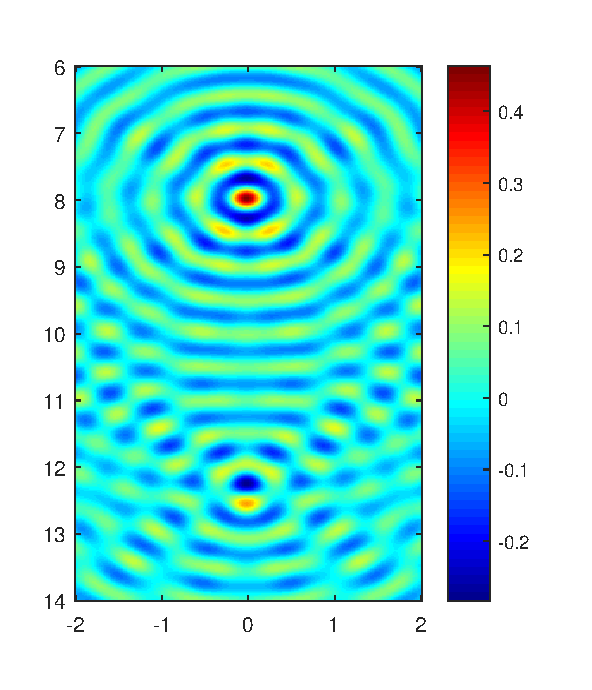
\includegraphics[width=0.4\textwidth]{./half/psf/in_imagesc.eps}
  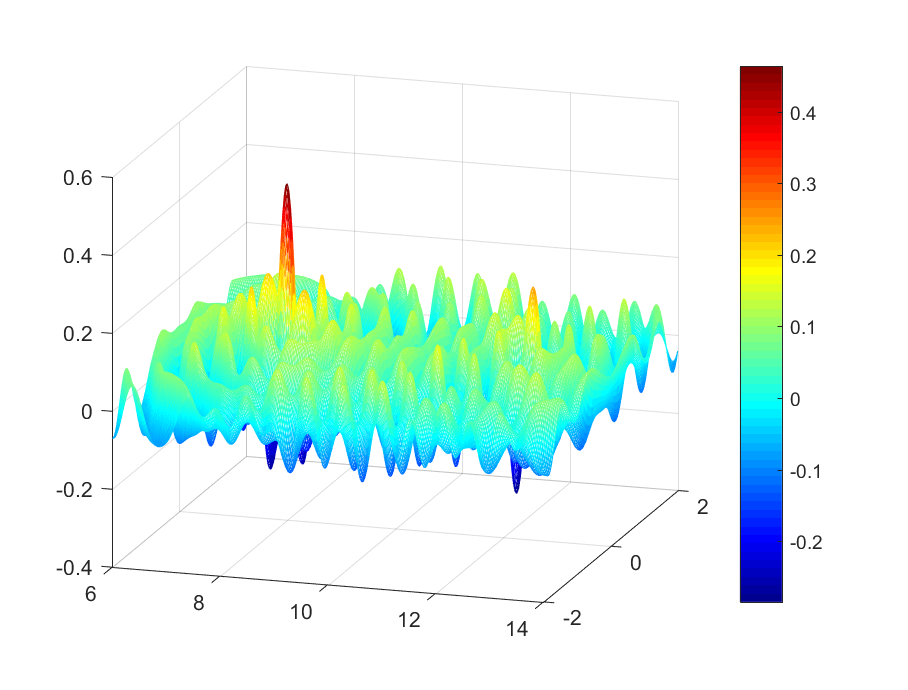
\includegraphics[width=12cm,height=6cm]{./waveguide1/psf_half/in_mesh.eps}
  \caption{$-\Im J_d(z,y)$,其中$G_{bp}(x,z)=G_{k_1}(x,z)$,源点$y_1\in L_1$.}\label{ImagPSF_half1}
\end{figure}
\begin{figure}[h]
  \centering
%  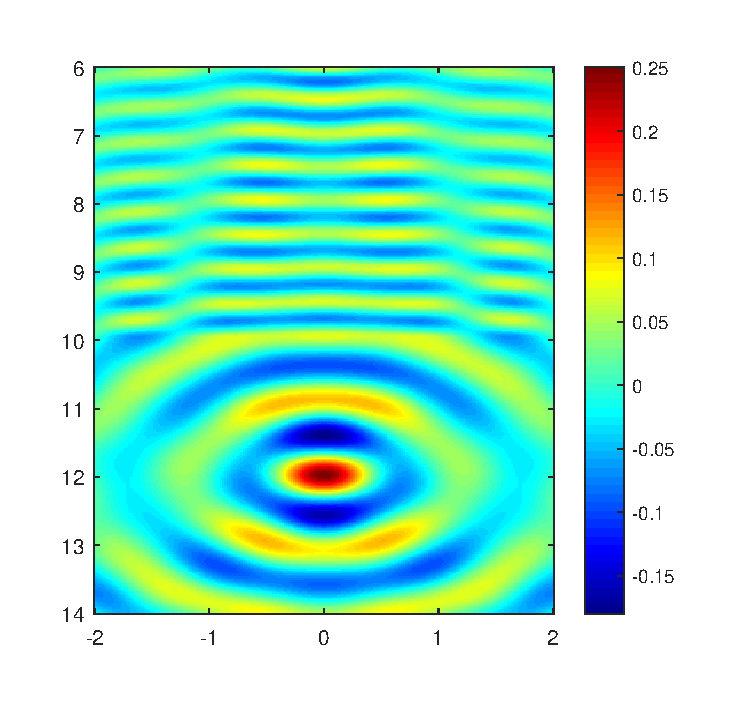
\includegraphics[width=0.4\textwidth]{./half/psf/out_imagesc.eps}
  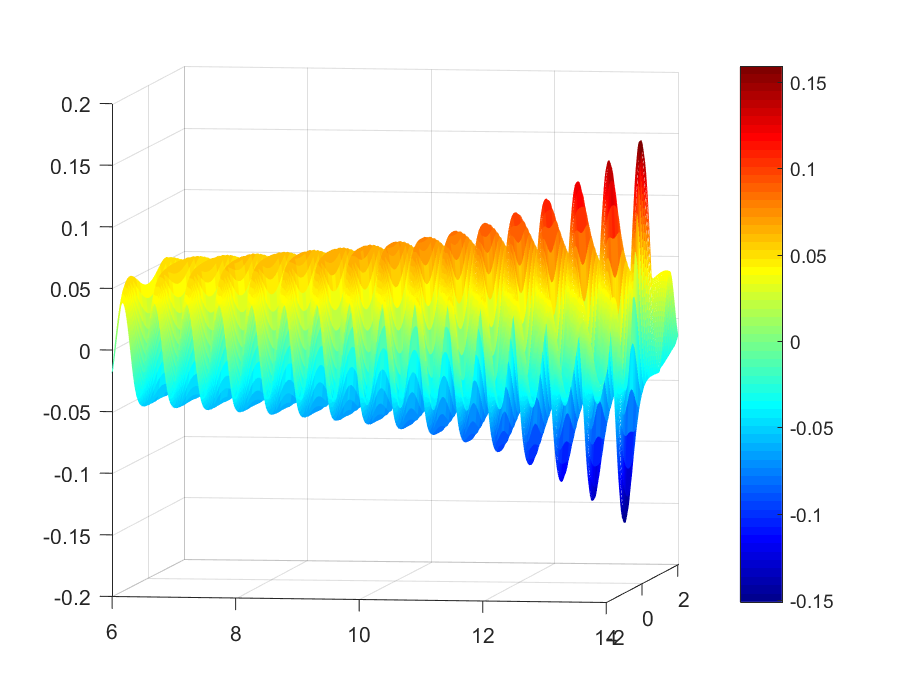
\includegraphics[width=12cm,height=6cm]{./waveguide1/psf_half/out_mesh.eps}
  \caption{$-\Im J_d(z,y)$,其中$G_{bp}(x,z)=G_{k_1}(x,z)$,源点$y_2\in L_2$.}\label{ImagPSF_half2}
\end{figure}


以上分析表明如果直接将文献\cite{ch_cw,ch_ha}中的想法推广到开波导情形,那么仅仅能够对位于开波导第一层内的障碍物进行有效成像,本章第五小节的数值测试结果也验证了这一事实,而对位于波导第二层的障碍物,选取$G_{k_1}(x,z)$作为反传播函数不再合适。因为在波导第二层波数为$k_2$,反传播函数$G_{k_1}(x,z)$的波数为$k_2$,明显不匹配。另外,由于同样的原因,我们选取$G_{k_2}(x,z)$ 也是不合适的。

\subsection{另一种想法:$G_{bp}(x,z)=G(x,z)$.}
一个比较自然的改进想法是选取$G_{bp}(x,z)=G(x,z)$,其中$G(x,y)$表示源点为$y$ 的Pekeris开波导Dirichlet 零边界格林函数,即
\begin{eqnarray}\label{G_Dirichlet}
\left\{
\begin{array}{lll}
  \Delta_xG(x,y)+k^2(x)G(x,y)=-\delta_z(y),&in&\R^2_+\\
  & &\\
  \left[G(\cdot,y)\right]_{\Gamma_h}=0,\ \ \left[\frac{\partial G(\cdot,y)}{\partial\nu}\right]_{\Gamma_h}=0 & &\\
  & &\\
  G(x,y)=0, &on&\Gamma_0
\end{array}
\right.
\end{eqnarray}
类似于格林函数$N(x,y)$,通过相同的手段,我们可以得到格林函数$G(x,y)$的积分表达式和波导模式展开表达式:
\begin{lemma}\label{f_Dirichlet}
令$\xi=\xi_1+\i\xi_2,\xi_1,\xi_2\in\R$,以及$\mu_j=\sqrt{k_j^2-\xi^2},j=1,2$,并记关于$\xi$的函数$N_h(\xi)$和$M_h(\xi)$如下所示
\begin{eqnarray}\label{NhMh}
 N_h(\xi)=\frac{\mu_1+\mu_2}{\mu_1-\mu_2}+e^{2\i\mu_1h},\ \
 M_h(\xi)=1+\frac{\mu_1+\mu_2}{\mu_1-\mu_2}e^{2\i\mu_1h},
\end{eqnarray}
则方程\ref{G_Dirichlet} 所定义的函数$G(x,y)$有如下表达式
\begin{eqnarray*}
G(x,y)=\left\{
\begin{array}{lll}
  \Phi_{k_1}(x,y)-\Phi_{k_1}(x,y')+S_1(x,y)&, &x\in L_1,y\in L_1\\
 S_2(x,y)&, &x\in L_2,y\in L_1\\
 K_1(x,y)&, &x\in L_1,y\in L_2\\
 \Phi_{k_2}(x,y)+K_2(x,y)&,&x\in L_2,y\in L_2
\end{array}
\right.
\end{eqnarray*}
其中$S_j(x,y),K_j(x,y),j=1,2$ 的表达式为
\begin{eqnarray*}
\left\{
\begin{array}{lll}
  S_1(x,y)&=&\frac{1}{2\pi}\int_{SIP}\frac{-\i}{2\mu_1}\frac{e^{2\i\mu_1h}\left[4\sin{(\mu_1x_2)\sin{(\mu_1y_2)}}\right]}{N_h(\xi)}
  e^{\i(x_1-y_1)\xi}d\xi\\
  & &\\
  S_2(x,y)&=&\frac{1}{2\pi}\int_{SIP}\frac{2e^{\i\mu_1h}\sin{(\mu_1y_2)}}{(\mu_1-\mu_2)N_h(\xi)}e^{\i\mu_2(x_2-h)+\i(x_1-y_1)\xi}d\xi\\
  & &\\
  K_1(x,y)&=&\frac{1}{2\pi}\int_{SIP}\frac{2e^{\i\mu_1h}\sin(\mu_1x_2)}{(\mu_1-\mu_2)N_h(\xi)}e^{\i\mu_2(y_2-h)+\i(x_1-y_1)\xi}d\xi\\
  & &\\
  K_2(x,y)&=&\frac{1}{2\pi}\int_{SIP}\frac{-\i}{2\mu_2}\frac{M_h(\xi)}{N_h(\xi)}e^{\i\mu_2(x_2+y_2-2h)+\i(x_1-y_1)\xi}d\xi
\end{array}
\right.
\end{eqnarray*}
\end{lemma}
\begin{remark}
同样地,格林函数$G(x,y)$ 的Fourier变换会出现极点,也就是函数$N_h(\xi)$ 的零点。直接验证可知,当$\xi\in\{\xi\in\R;|\xi|>k_1,|\xi|<k_2\}$ 时,
$N_h(\xi)\neq0$。于是当$\xi\in\R$时,$N_h(\xi)$ 的零点仅仅分布在区间$[k_2,k_1]$,或区间$[-k_1,-k_2]$上。特别地,$\xi=\pm k_1$是$N_h(\xi)$的零点,但是我们同时注意到当$\xi=\pm k_1$时,$\hat G_y(\xi,x_2)$中对应于$N_h(\xi)$的分子同样为零,并不会给后面的分析带来麻烦。当$\xi=\pm k_2$ 时,
\begin{equation}
  N_h(\xi)=0\ \ \Rightarrow\ \ \cos\left(\sqrt{k_1^2-k_2^2}h\right)=0
\end{equation}
由该方程可解出频率$\omega=\frac{c_1c_2}{\sqrt{c_2^2-c_1^2}}\frac{(n+\frac{1}{2})\pi}{h}$,称为截断频率。一般地,我们假设$\cos\left(\sqrt{k_1^2-k_2^2}h\right)\neq0$ 以保证模型不会产生截断频率。当$\xi\in(k_2,k_1)$ 时,$N_h(\xi)=0$等价于
\begin{equation}
  \tan{\left(\sqrt{k_1^2-\xi^2}h\right)}=-\frac{\sqrt{k_1^2-\xi^2}}{\sqrt{\xi^2-k_2^2}}
\end{equation}
记$N_h(\xi)$在区间$(k_2,k_1)$上的零点个数为$M$, 则由上式可知,$M\leq\left[\sqrt{k_1^2-k_2^2}h/\pi\right]$。 我们记这$M$个零点为$\xi_1,\ldots,\xi_M$,易验证$N'_h(\xi_m)\neq0$,于是这$M$个零点都是$N_h(\xi)$的一阶零点,它们对应了函数$G(x,y)$的$M$ 个波导模式。

\end{remark}
\begin{lemma}[关于$G(x,y)$的波导模式展开]\label{Dirichlet_Mode}
设$\xi_m$, $m=1,\ldots,M$是函数$N_h(\xi)$在区间$(k_2,k_1)$ 上的$M$ 个实根,并记$\mu_{1m}=\mu_1(\xi_m),\mu_{2m}=\mu_2(\xi_m)$,则$G(x,y)$ 的波导模式展开为
\begin{equation*}
  G(x,y)=G_g(x,y)+G_{rad}(x,y)
\end{equation*}
其中$G_g(x,y)=\sum\limits_{m=1}^M G_m(x,y)$,且
\begin{eqnarray}
\left\{
\begin{array}{lll}
  G_m(x,y)&=&\frac{\mu_{2m}}{\xi_m(1-\i\mu_{2m}h)}g(x_2,\xi_m)g(y_2,\xi_m)e^{\i|x_1-y_1|\xi_m}\\
& &\\
 G_{rad}(x,y)&=&\frac{\ii}{\pi}\int_{\ii\infty}^{k_2}\frac{\mu_2 g(x_2,\xi)g(y_2,\xi)}{(k_1^2-k_2^2)\cos^2(\mu_1h)+\mu_2^2}e^{\ii|x_1-y_1|\xi}d\xi
\end{array}
\right.
\end{eqnarray}
其中$G_m(x,y)$中对应于$\xi_m\in(k_2,k_1)$的$g(x_2,\xi_m)$ 表达式如下
 \begin{eqnarray*}
 g(x_2,\xi_m):=\left\{
 \begin{array}{lll}
   \sin(\mu_{1m}x_2),& &x_2\in(0,h)\\
   & &\\
   \sin(\mu_{1m}h)e^{\i\mu_{2m}(x_2-h)},& &x_2\in(h,+\infty)
 \end{array}
 \right.
 \end{eqnarray*}
此外$G_{rad}(x,y)$中有向积分区间$[\i\infty,k_2]:=\{\xi;\xi\in[0,k_2],\ \ \mbox{或}\xi=\i\eta$,$\eta\in(0,+\infty)\}$,以及对应于$\xi\in[\i\infty,k_2]$的函数$g(x_2,\xi)$ 如下
 \begin{eqnarray*}
 g(x_2,\xi):=\left\{
 \begin{array}{lll}
   \sin(\mu_1x_2),& &x_2\in(0,h)\\
   & &\\
   \sin(\mu_1h)\cos[\mu_2(x_2-h)]+\frac{\mu_1}{\mu_2}\cos(\mu_1h)\sin[\mu_2(x_2-h)],& &x_2\in(h,+\infty)
 \end{array}
 \right.
 \end{eqnarray*}
\end{lemma}


我们期待选取$G(x,z)$为反传播函数可以解决之前遇到的波数不一致问题,数值测试结果也间接表明这种方法或许可取。设定测试参数与之前完全一样,测试结果如图\ref{ImagPSF_wg1}和\ref{ImagPSF_wg2}所示。从测试结果来看,选取函数$G(x,z)$ 作为反传播函数能够很好地解决问题\ref{pro_psf}。
\begin{figure}[h]
  \centering
%  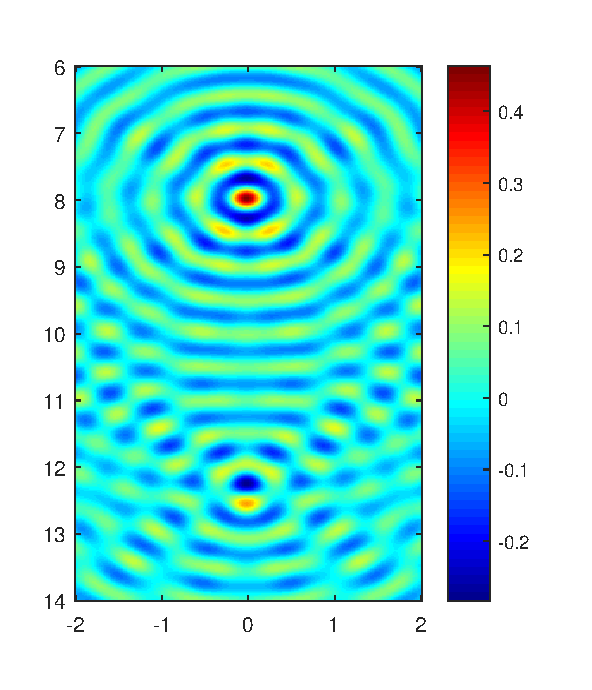
\includegraphics[width=0.4\textwidth]{./half/psf/in_imagesc.eps}
  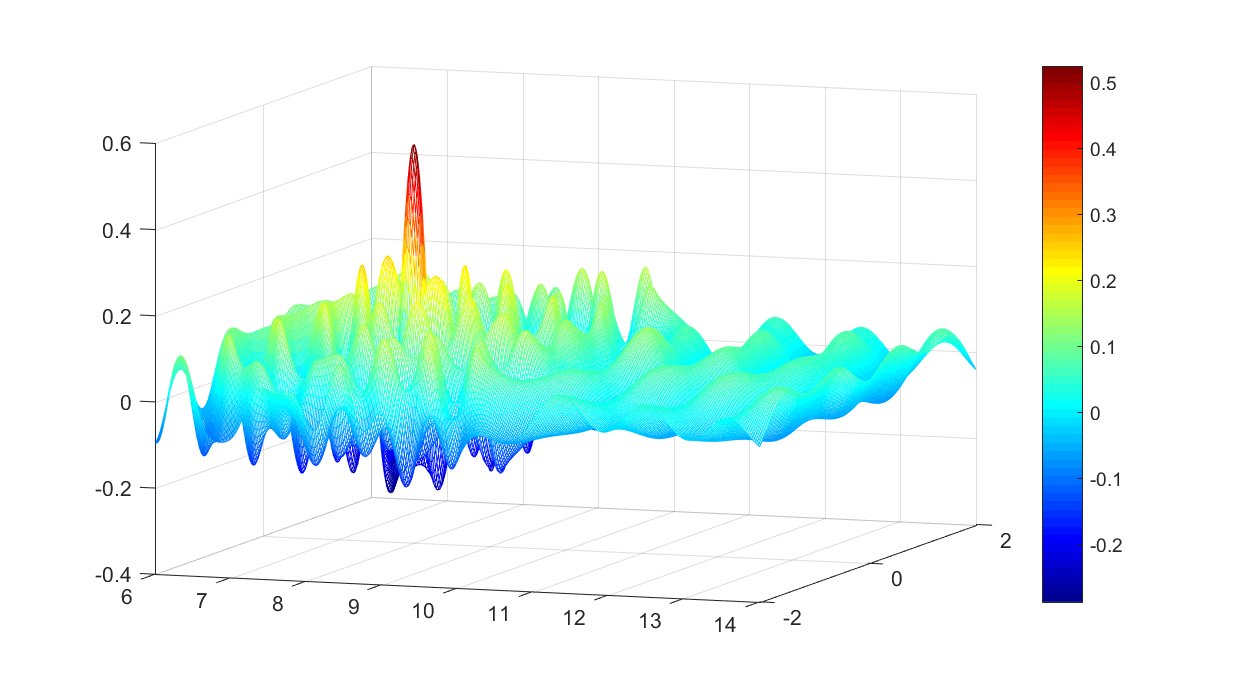
\includegraphics[width=13cm,height=5cm]{./waveguide1/psf_waveguide/in_mesh.eps}
  \caption{$-\Im J_d(z,y)$,其中$G_{bp}(x,z)=G(x,z)$,源点$y_1\in L_1$.}\label{ImagPSF_wg1}
\end{figure}
\begin{figure}[h]
  \centering
%  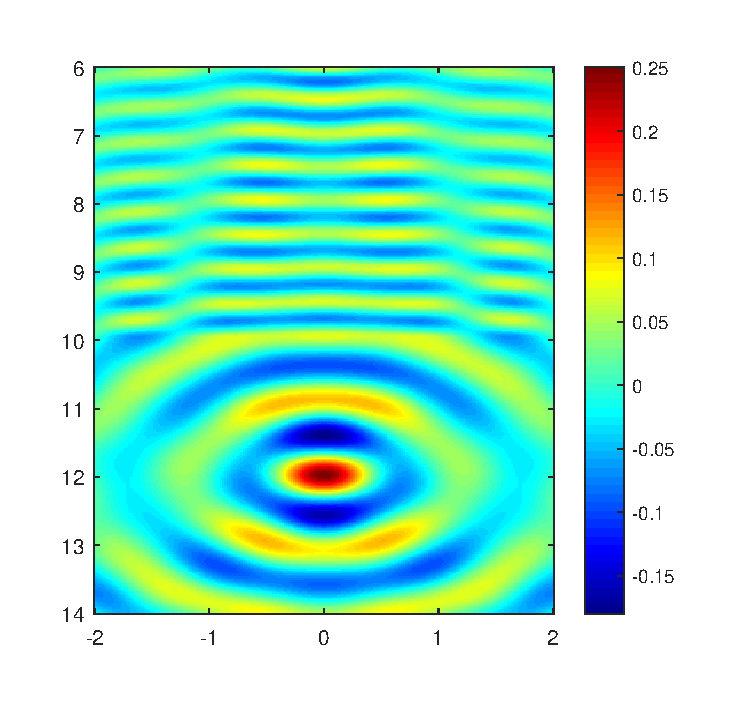
\includegraphics[width=0.4\textwidth]{./half/psf/out_imagesc.eps}
  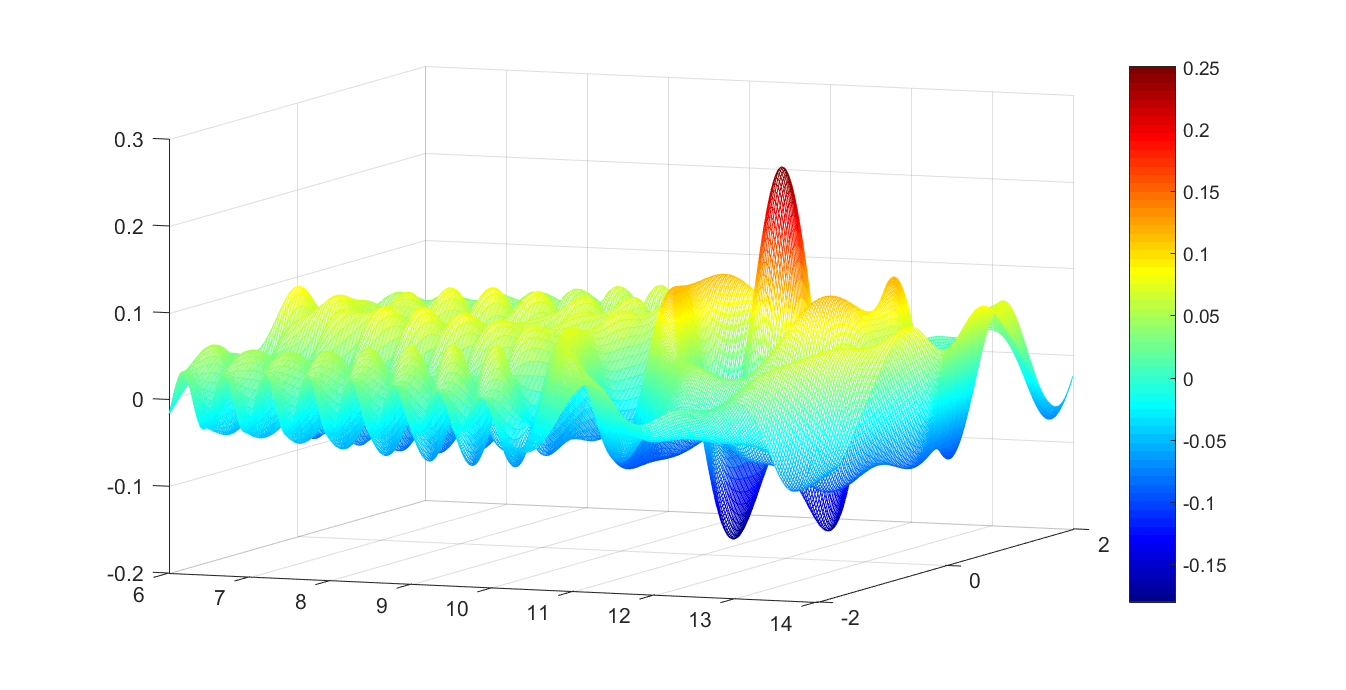
\includegraphics[width=13cm,height=5cm]{./waveguide1/psf_waveguide/out_mesh.eps}
  \caption{$-\Im J_d(z,y)$,其中$G_{bp}(x,z)=G(x,z)$,源点$y_2\in L_2$.}\label{ImagPSF_wg2}
\end{figure}
\section{Pekeris开波导逆时偏移算法}
通过对点扩散函数的分析和测试,我们提出针对Pekeris开波导障碍物成像问题的逆时偏移算法:
\begin{algorithm}\label{alg_wg}
设$\Omega$为采样区域,令$u^s(x_r,x_s)$ 为在接收点$x_r$收到的由源点$x_s$ 所激发的散射数据,其中$x_r,x_s\in\Gamma_0^d;r=1,\ldots,N_r;s=1,\ldots,N_s$.\\
$1^\circ$ 反传播: 对$s=1,\ldots,N_s$,计算反传播场
\begin{equation}
  v_b(z,x_s)=\frac{|\Gamma_0^d|}{N_r}\sum\limits_{r=1}^{N_r}\frac{\partial G(x_r,z)}{\partial x_2(x_r)}\overline{u^s(x_r,x_s)},\  \  \forall z\in\Omega.
\end{equation}
若令$N_r\rightarrow0$,则上式可看做如下积分的数值近似,
\begin{equation}
  \hat v_b(z,x_s)=\int_{\Gamma_0^d}\frac{\partial G(x_r,z)}{\partial x_2(x_r)}\overline{u^s(x_r,x_s)}ds(x_r)
\end{equation}
$2^\circ$ 互相关: 对$z\in\Omega$,计算成像函数
\begin{equation}
  I_d(z)=\Im\left\{\frac{|\Gamma_0^d|}{N_s}\sum\limits_{s=1}^{N_s}\frac{\partial G(x_s,z)}{\partial x_2(x_s)}v_b(z,x_s)
  \right\}.
\end{equation}
将$v_b(z,x_s)$的表达式代入$I_d(z)$,可得
\begin{equation}\label{Id_wg}
  I_d(z)=\Im\left\{\frac{|\Gamma_0^d|}{N_s}\frac{|\Gamma_0^d|}{N_r}\sum\limits_{s=1}^{N_s}\sum\limits_{r=1}^{N_r}\frac{\partial G(x_s,z)}{\partial x_2(x_s)}\frac{\partial G(x_r,z)}{\partial x_2(x_r)}\overline{u^s(x_r,x_s)}
  \right\}.
\end{equation}
成像函数\eqref{Id_wg} 将用于下节所有的数值算例测试。
若令$N_s,N_r\rightarrow\infty$,则上式可看做如下积分的数值近似,
\begin{equation}\label{Id_wg_hat}
  \hat I_d(z)=\Im\int_{\Gamma_0^d}\int_{\Gamma_0^d}\frac{\partial G(x_s,z)}{\partial x_2(x_s)}
  \frac{\partial G(x_r,z)}{\partial x_2(x_r)}\overline{u^s(x_r,x_s)}ds(x_r)ds(x_s).
\end{equation}
\end{algorithm}

\section{数值测试}

在本小节我们将通过数值算例来测试算法\ref{alg_wg} 对嵌入在开波导结构中障碍物的成像效果。 散射数据$u^s(x_r,x_s)$ 由标准的Nystr\"om 方法生成。在求解边界$\Gamma_D$上的积分方程时,我们每个波长布置10个离散点。本章主要依旧采用如下具有参数表示的障碍物边界作为测试算例,分别为$P$叶风扇形状、 圆形、花生形状以及边角被光滑后的方块形状,它们的参数表达分别如下
\begin{eqnarray}\label{obstacle_example2}
\left\{
\begin{array}{lll}
x_1=r(\theta)\cos\theta&,& x_2=r(\theta)\sin\theta,\ \ \mbox{其中}\ \ r(\theta)=1+0.2\cos(p\theta),\\
x_1=\rho\cos{\theta}&,& x_2=\rho\sin{\theta},\\
x_1=\cos{\theta}+0.2\cos{3\theta}&,& x_2=\sin{\theta}+0.2\sin{3\theta},\\
x_1=\cos^3\theta+\cos{\theta}&,& x_2=\sin^3\theta+\sin{\theta}.
\end{array}
\right.
\end{eqnarray}
\subsection{障碍物$D\subset L_1$.}
在本小节中,我们先考虑障碍物位于Pekeris开波导第一层$L_1$,即假设$D\subset L_1$。 我们令$h=10,d=50$,且源点$x_s$ 和接收点$x_r$ 在$\Gamma_0^d$ 上均匀分布,其中$\Gamma_0^d=\{(x_1,x_2)\in\R^2;x_1\in(-d,d),x_2=0\}$。 采样区域为$\Omega=[-2,2]\times[6,10]$,且我们采用$201\times201$ 的均匀采样。探测频率为$k_1=4\pi,k_2=2\pi$。 源点和接收点个数为$N_s=256,N_r=256$。
\begin{example}[不同形状]\label{wg_ex1}
在本算例中,我们以声软障碍物为例测试位于Pekeris 开波导第一层具有不同形状的障碍物,例如4叶风扇形状,矩形形状,花生形状和椭圆形状,算法\ref{alg_wg}的成像效果。与此同时,我们也同时测试当所采用的反传播函数为$G_{k_1}(x,z)$ 时,即如下成像函数:
\begin{equation}\label{Id_half}
   I_d^{k_1}(z)=\Im\left\{\frac{|\Gamma_0^d|}{N_s}\frac{|\Gamma_0^d|}{N_r}\sum\limits_{s=1}^{N_s}\sum\limits_{r=1}^{N_r}\frac{\partial G_{k_1}(x_s,z)}{\partial x_2(x_s)}\frac{\partial G_{k_1}(x_r,z)}{\partial x_2(x_r)}\overline{u^s(x_r,x_s)}
  \right\}.
\end{equation}
的成像效果。

测试结果如图\ref{fig_wg_ex1}所示,当障碍物位于Pekeris开波导第一层$L_1$时,两种成像函数都能够对不同形状的声软障碍物做到有效成像。除此之外,通过对比,我们可以看到:在相同参数下,算法\ref{alg_wg}的成像函数\eqref{Id_wg}的成像效果要远远好于采用函数$G_{k_1}(x,z)$作为反传播函数时所对应的成像函数\eqref{Id_half}。事实上,成像函数\ref{Id_wg}的成像值几乎都是正值,具有更好的稳定性,而且其不仅仅确定了声软障碍物的上边界,对于下边界以及侧边界也可以做到稍微粗浅的成像。
\end{example}

\begin{figure}[h]
  \centering
  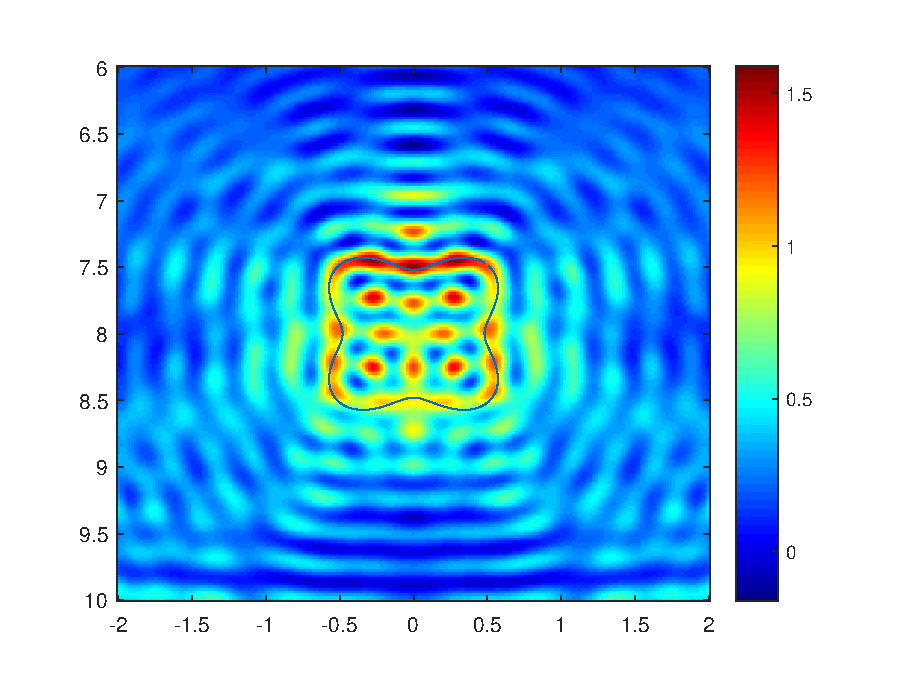
\includegraphics[width=0.23\textwidth]{./waveguide1/example1/In_soft_pleaf1.eps}
  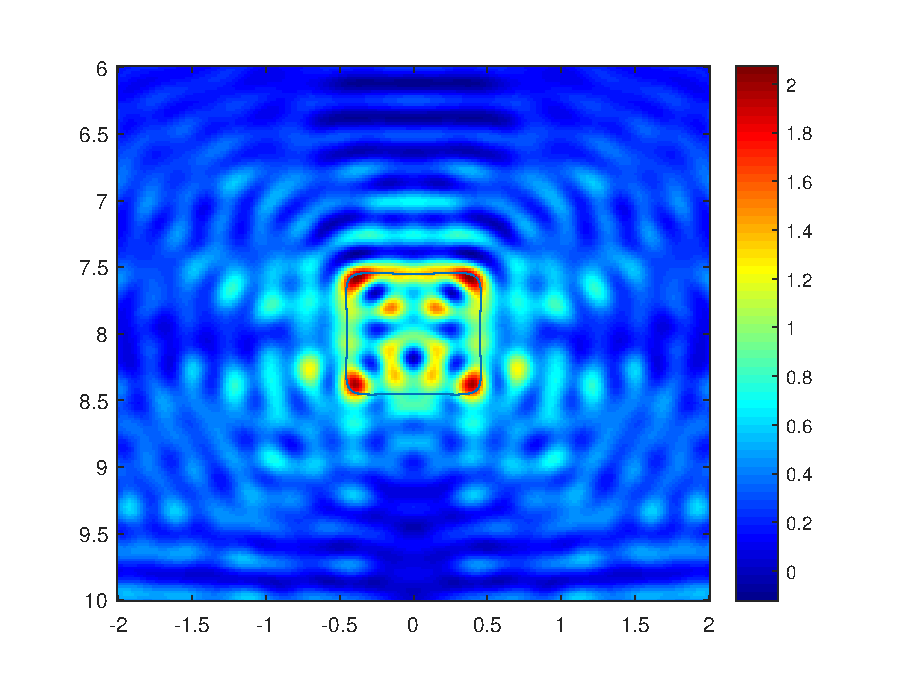
\includegraphics[width=0.23\textwidth]{./waveguide1/example1/In_soft_square1.eps}
  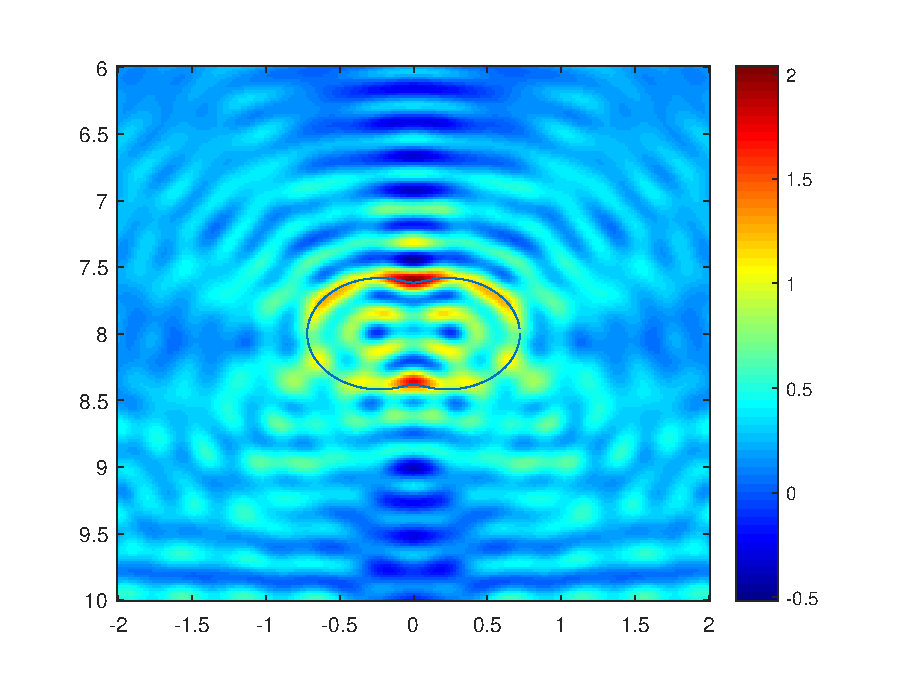
\includegraphics[width=0.23\textwidth]{./waveguide1/example1/In_soft_peanut.eps}
  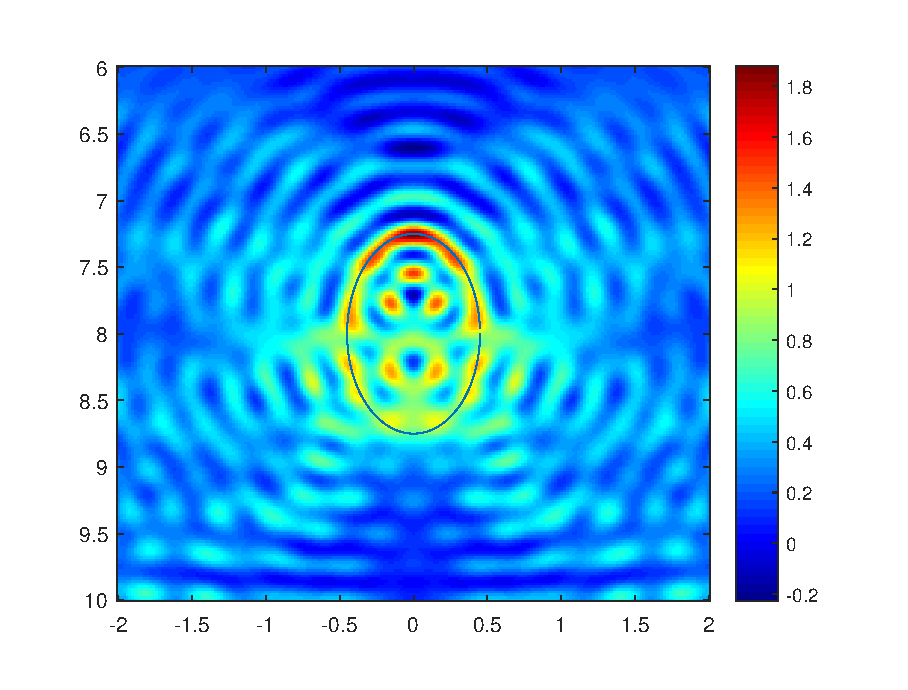
\includegraphics[width=0.23\textwidth]{./waveguide1/example1/In_soft_circle1.eps}
  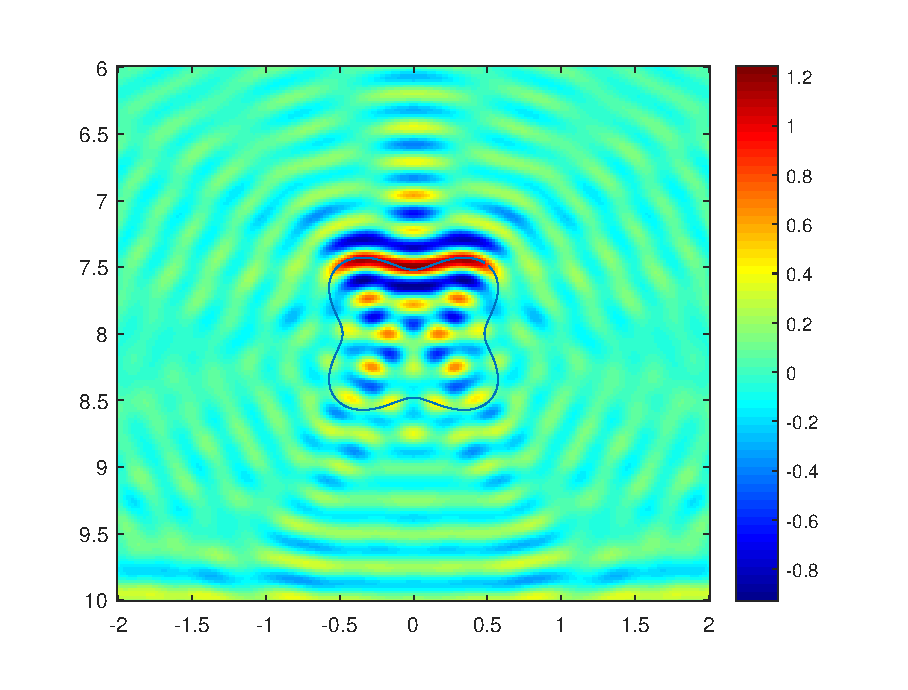
\includegraphics[width=0.23\textwidth]{./waveguide1/example1/In_soft_pleaf1_half.eps}
  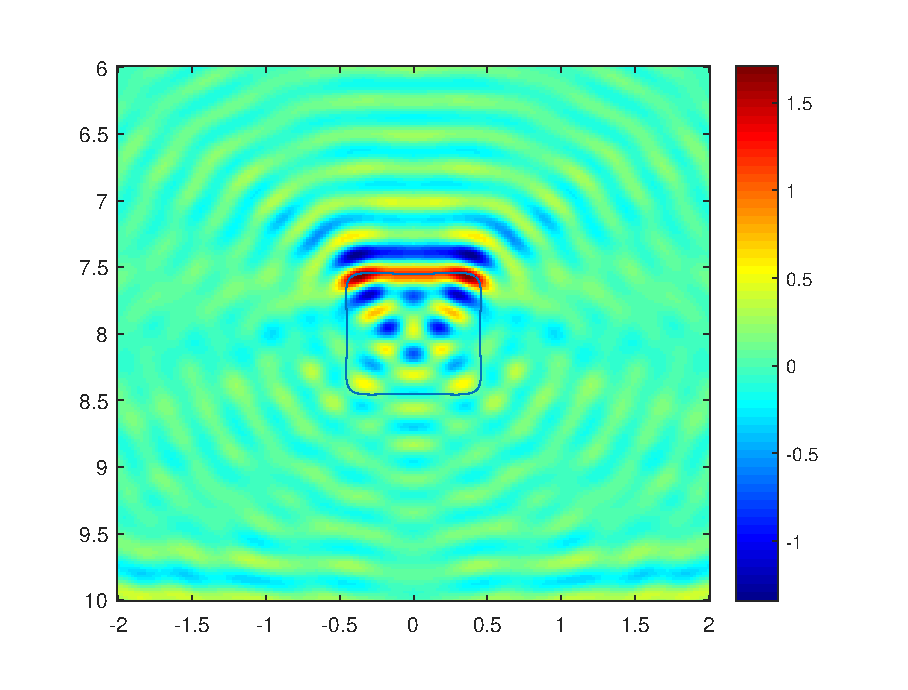
\includegraphics[width=0.23\textwidth]{./waveguide1/example1/In_soft_square1_half.eps}
  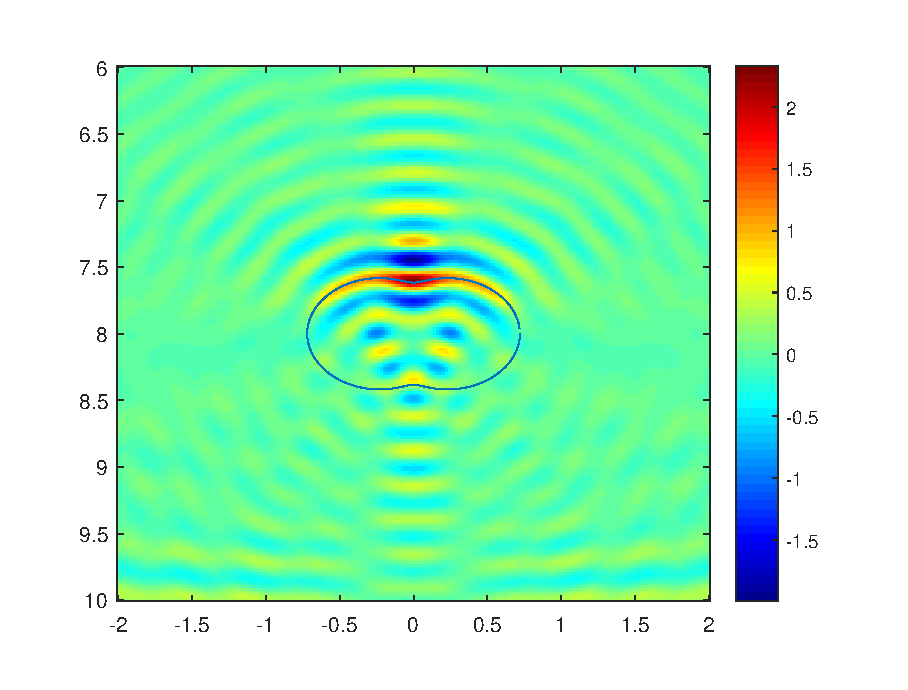
\includegraphics[width=0.23\textwidth]{./waveguide1/example1/In_soft_peanut_half.eps}
  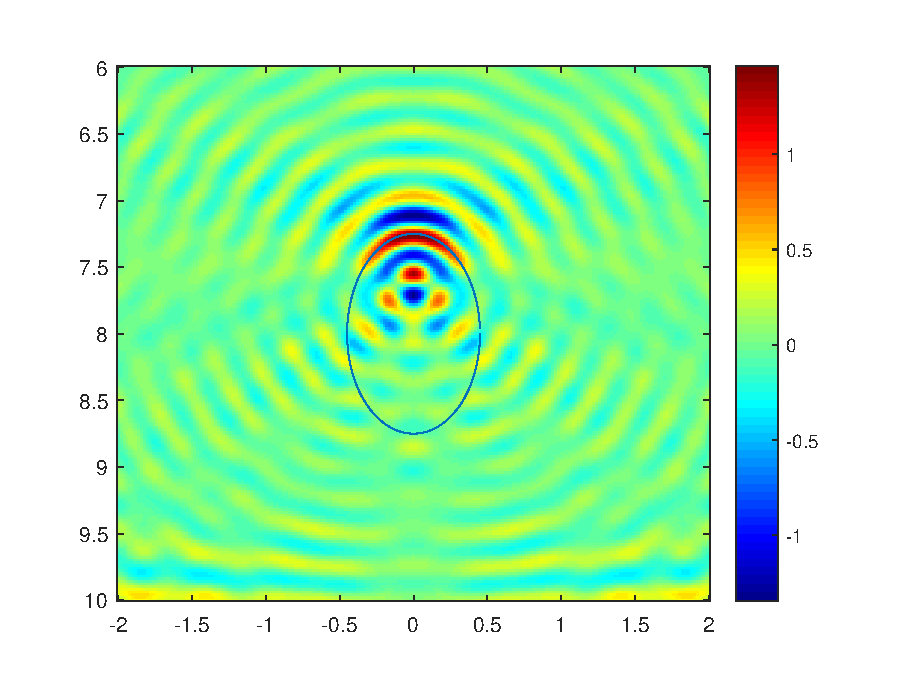
\includegraphics[width=0.23\textwidth]{./waveguide1/example1/In_soft_circle1_half.eps}
  \caption{算例\ref{wg_ex1}:测试不同形状的声软障碍物成像效果,从左到右依次为4 叶风扇、矩形、花生以及椭圆形状,其中第一行为算法\ref{alg_wg}成像函数\ref{Id_wg}的成像效果,第二行为反传播函数是函数$G_{k_1}(x,z)$时所对应成像函数\ref{Id_half}的成像效果。}\label{fig_wg_ex1}
\end{figure}

\begin{example}[不同边界类型]\label{wg_ex2}
在本算例中,我们以圆形障碍物为例,验证算法\ref{alg_wg}对位于Pekeris 开波导第一层具有不同边界类型的障碍物的成像效果。例如声软障碍物,声硬障碍物,折射系数为$n(x)$ 的可穿透障碍物,阻尼系数为$\eta(x)$的阻抗边界障碍物。对于可穿透障碍物成像,我们假设折射系数$n(x)$ 为:
\begin{eqnarray*}
n(x)=\left\{
\begin{array}{lll}
  0.5&,&x\in D\\
  1&,&x\in\R_+^2\backslash\overline D
\end{array}
\right.
\end{eqnarray*}
对于阻抗边界障碍物,我们假设在上半边界$\eta(x)=1$,在下半边界$\eta(x)=2$。

数值测试结果如图\ref{fig_wg_ex2}所示,结果表明:在不知道障碍物的任何先验信息的情况下,如是否可穿透,以及不可穿透障碍物的边界条件,两种成像函数都能够对不同类型的圆形障碍物做到有效成像。类似地,算法\ref{alg_wg}所对应成像函数\eqref{Id_wg}的成像效果依旧远远好于当反传播函数为$G_{k_1}(x,z)$时所对应成像函数\eqref{Id_half}的成像效果。从图\ref{fig_wg_ex2}第四列的对比可以看出,即使障碍物为可穿透类型时,成像函数\eqref{Id_wg}也明显优于\eqref{Id_half},因为其不仅能对上下边界进行成像,而且对于侧边界也有不错的成像效果。
\end{example}
\begin{figure}[htbp]
  \centering
  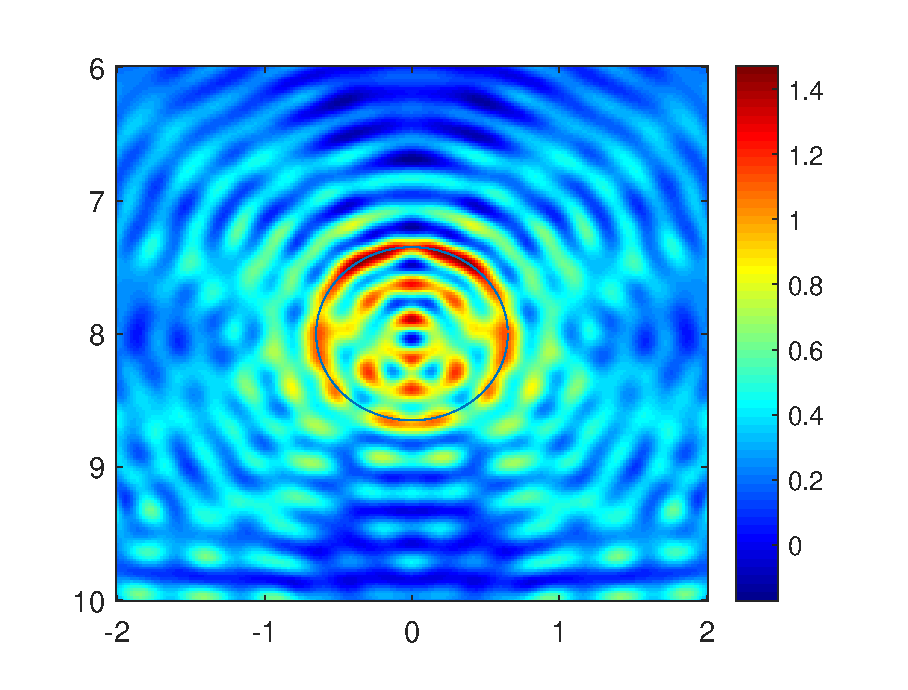
\includegraphics[width=0.23\textwidth]{./waveguide1/example2/In_Circle_Soft.eps}
  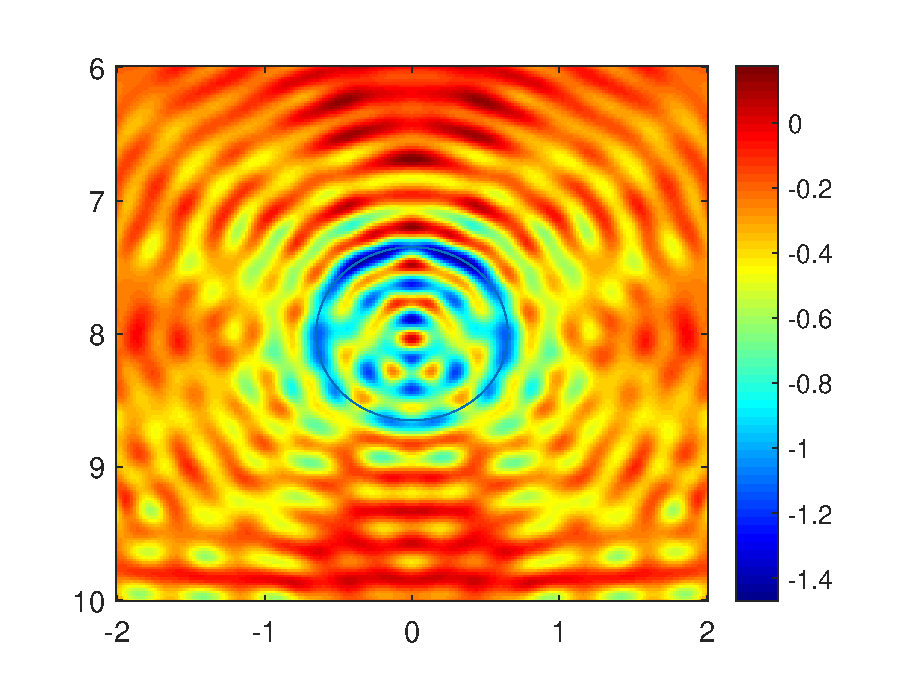
\includegraphics[width=0.23\textwidth]{./waveguide1/example2/In_Circle_Hard.eps}
  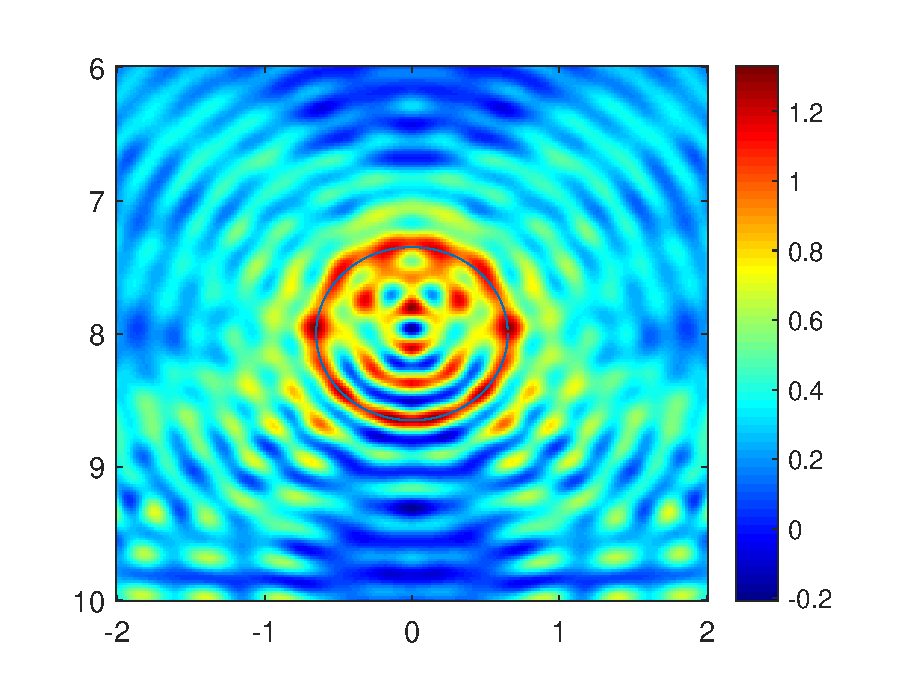
\includegraphics[width=0.23\textwidth]{./waveguide1/example2/In_Circle_Imp.eps}
  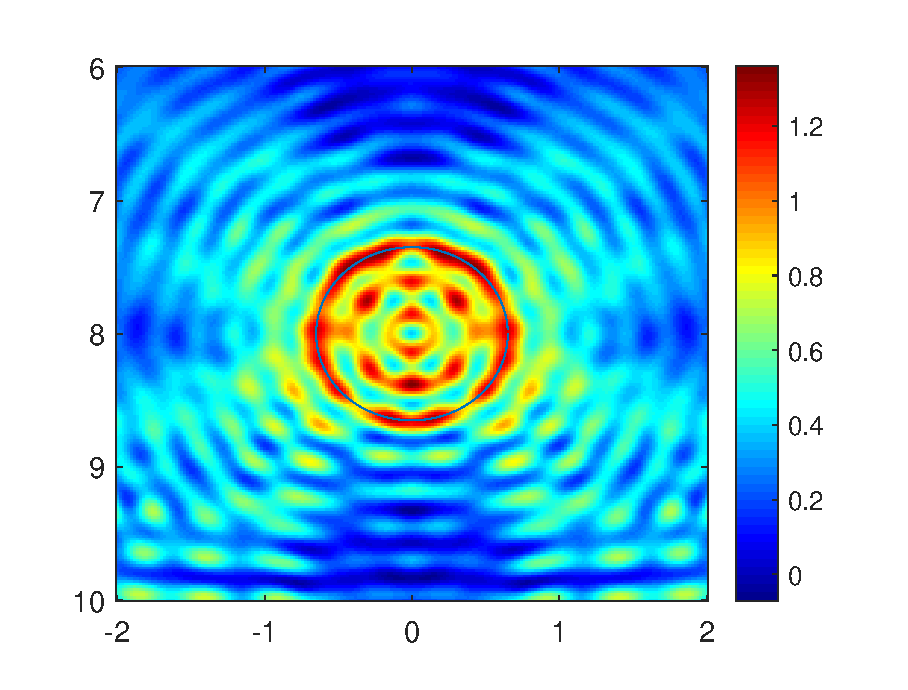
\includegraphics[width=0.23\textwidth]{./waveguide1/example2/In_Circle_Tran.eps}
  \includegraphics[width=0.23\textwidth]{./waveguide1/example2/In_Circle_Soft_half.eps}
  \includegraphics[width=0.23\textwidth]{./waveguide1/example2/In_Circle_Hard_half.eps}
  \includegraphics[width=0.23\textwidth]{./waveguide1/example2/In_Circle_Imp_half.eps}
  \includegraphics[width=0.23\textwidth]{./waveguide1/example2/In_Circle_Tran_half.eps}
  \caption{算例\ref{wg_ex2}:测试不同类型不同边界的障碍物:前面三个从左到右依次为声软障碍物、声硬障碍物、阻尼系数为$\eta(x)$的阻抗边界障碍物,最后一个为折射系数为$n(x)$的可穿透障碍物,其中第一行为算法\ref{alg_wg}成像函数\ref{Id_wg}的成像效果,第二行为反传播函数是函数$G_{k_1}(x,z)$时所对应成像函数\ref{Id_half}的成像效果。}\label{fig_wg_ex2}
\end{figure}


\begin{example}[抗噪性测试]\label{wg_ex3}
在本算例中,我们测试当在$\Gamma_0^d$上做采集到的散射数据$u^s(x_r,x_s)$带有噪音时,对嵌入在Pekeris开波导第一层$L_1$的障碍物$D$,算法\ref{alg_wg}的成像函数\eqref{Id_wg}的抗噪性能。一般地,我们假设$u^s_{noise}(x_r,x_s)$ 为如下带有高斯噪音的散射数据:
$$ u^s_{noise}(x_r,x_s)=u^s(x_r,x_s)+v_{noise},$$
其中$v_{noise}$为满足如下分布的高斯噪音:
$$v_{noise}=\mu \max{|u^s|}\epsilon,\ \ \epsilon\sim N(0,1).$$

我们第一个测试的是4-叶风扇形状的声软障碍物,测试结果如图\ref{fig_wg_ex3_1}所示:假设从左到右噪音水平$\mu$按如下数值依次递增:$0.1,0.2,0.4,0.6$,其中第一行为单频测试结果,测试频率为$k_1=4\pi,k_2=2\pi$;第二行为多频测试结果,测试频率为$k_2=\frac{1}{2}k_1,k_1=2\pi+0.4n\pi,n=0,1\ldots,9$。结果表明:算法\ref{alg_wg}中的成像函数\ref{Id_wg}具有十分良好的抗噪性能;此外,当采集到的数据为多个频率时,将多个频率的成像函数直接进行相加,能够很好地改善成像效果,大大提高对噪音的抵抗能力;最后多频测试结果还表明算法\ref{alg_wg}在确定所探寻的障碍物的位置时是十分准确而不带偏差的。

我们第二个测试的是圆形的折射系数$n(x)$为
\begin{eqnarray*}
	n(x)=\left\{
	\begin{array}{lll}
		0.5&,&x\in D\\
		1&,&x\in\R_+^2\backslash\overline D
	\end{array}
	\right.
\end{eqnarray*}
的可穿透障碍物,测试结果如图\ref{fig_wg_ex3_2}所示:噪音水平和测试频率的设置与上一个测试算例一模一样,第一、二行分别为单频和多频测试结果。测试结果表明:多频能够极大提高算法\ref{alg_wg}的抗噪音性能;此外,对于可穿透障碍物而言,算法的成像效果要优于不可穿透障碍物,如声软障碍物,这也是符合预期的。
\end{example}
\begin{figure}[htbp]
  \centering
  \includegraphics[width=0.23\textwidth]{./waveguide1/example3/In_soft_pleaf1_2.eps}
  \includegraphics[width=0.23\textwidth]{./waveguide1/example3/In_soft_pleaf1_4.eps}
  \includegraphics[width=0.23\textwidth]{./waveguide1/example3/In_soft_pleaf1_5.eps}
  \includegraphics[width=0.23\textwidth]{./waveguide1/example3/In_soft_pleaf1_6.eps}
  \includegraphics[width=0.23\textwidth]{./waveguide1/example3/In_soft_pleaf1_4_multi.eps}
  \includegraphics[width=0.23\textwidth]{./waveguide1/example3/In_soft_pleaf1_6_multi.eps}
  \includegraphics[width=0.23\textwidth]{./waveguide1/example3/In_soft_pleaf1_8_multi.eps}
  \includegraphics[width=0.23\textwidth]{./waveguide1/example3/In_soft_pleaf1_10_multi.eps}
  \caption{算例\ref{wg_ex3}:测试算法\ref{alg_wg}的抗噪音性能:目标障碍物为4-叶风扇形声软障碍物,噪音水平$\mu$从左到右按如下数值依次递增:$0.1,0.2,0.4,0.6$。其中第一行为单频测试结果,测试频率为:$k_1=4\pi,k_2=2\pi$;第二行为多频测试结果,测试频率为:$k_2=\frac{1}{2}k_1,k_1=2\pi+0.4n\pi,n=0,1\ldots,9$。}\label{fig_wg_ex3_1}
\end{figure}
\begin{figure}[htbp]
  \centering
  \includegraphics[width=0.23\textwidth]{./waveguide1/example3/In_transmission_circle_2.eps}
  \includegraphics[width=0.23\textwidth]{./waveguide1/example3/In_transmission_circle_3.eps}
  \includegraphics[width=0.23\textwidth]{./waveguide1/example3/In_transmission_circle_4.eps}
  \includegraphics[width=0.23\textwidth]{./waveguide1/example3/In_transmission_circle_5.eps}
  \includegraphics[width=0.23\textwidth]{./waveguide1/example3/In_transmission_circle_2_multi.eps}
  \includegraphics[width=0.23\textwidth]{./waveguide1/example3/In_transmission_circle_4_multi.eps}
  \includegraphics[width=0.23\textwidth]{./waveguide1/example3/In_transmission_circle_6_multi.eps}
  \includegraphics[width=0.23\textwidth]{./waveguide1/example3/In_transmission_circle_8_multi.eps}
  \caption{算例\ref{wg_ex3}:测试算法\ref{alg_wg}的抗噪音性能:目标障碍物为圆形的可穿透障碍物,噪音水平$\mu$从左到右按如下水平依次递增:$0.1,0.2,0.4,0.6$。其中第一行为单频测试结果,测试频率为:$k_1=4\pi,k_2=2\pi$;第二行为多频测试结果,测试频率为:$k_2=\frac{1}{2}k_1,k_1=2\pi+0.4n\pi,n=0,1\ldots,9$。}\label{fig_wg_ex3_2}
\end{figure}
\begin{remark}
	从本小节的数值算例可以看出,当目标障碍物$D$嵌入在Pekeris开波导第一层时,我们在上节所提出的算法\ref{alg_wg}能够对不同类型不同边界的障碍物进行有效成像,而且具有良好的抗噪性能。多频测试结果表明了算法定位目标的准确性以及多频能极大提高算法性能。除此之外,我们也发现,如果仅仅是探寻开波导第一层$L_1$内的障碍物,那么函数$G_{k_1}(x,z):=\Phi_{k_1}(x,z)-\Phi_{k_1}(x,z')$也是一种可选的反传播函数,其好处是反传播函数的计算速度极快以及计算精度较高。
\end{remark}
\subsection{障碍物$D\subset L_2$.}
在本小节中,我们考虑障碍物位于Pekeris开波导第二层$L_2$,即假设$D\subset L_2$。我们令$h=10,d=50$,且源点$x_s$ 和接收点$x_r$依旧 在$\Gamma_0^d$上均匀分布,其中$\Gamma_0^d=\{(x_1,x_2)\in\R^2;x_1\in(-d,d),x_2=0\}$。 采样区域为$\Omega=[-2,2]\times[10,14]$,且我们采用$201\times201$ 的均匀采样。为提高分辨率,取探测频率为$k_1=8\pi,k_2=4\pi$。 源点和接收点个数为$N_s=256,N_r=256$。
\begin{example}[不同边界类型]\label{wgout_ex1}
在本算例中,我们以圆形障碍物为例,验证算法\ref{alg_wg}对位于Pekeris 开波导第二层具有不同边界类型的障碍物的成像效果。例如声软障碍物,声硬障碍物,折射系数为$n(x)$ 的可穿透障碍物,阻尼系数为$\eta(x)$的阻抗边界障碍物。对于可穿透障碍物成像,我们假设折射系数$n(x)$ 为:
\begin{eqnarray*}
n(x)=\left\{
\begin{array}{lll}
  0.5&,&x\in D\\
  1&,&x\in\R_+^2\backslash\overline D
\end{array}
\right.
\end{eqnarray*}
对于阻抗边界障碍物,我们假设在上半边界$\eta(x)=1$,在下半边界$\eta(x)=2$。与之前一样,我们将使用相同的参数设定,来测试当反传播函数为$G_{k_1}(x,z)$时所对应的成像函数\eqref{Id_half}的成像效果。除此之外,我们将同样考虑反传播函数为$G_{k_2}(x,z):=\Phi_{k_2}(x,z)-\Phi_{k_2}(x,z')$时如下成像函数:
\begin{equation}\label{Id_half2}
I_d^{k_2}(z)=\Im\left\{\frac{|\Gamma_0^d|}{N_s}\frac{|\Gamma_0^d|}{N_r}\sum\limits_{s=1}^{N_s}\sum\limits_{r=1}^{N_r}\frac{\partial G_{k_2}(x_s,z)}{\partial x_2(x_s)}\frac{\partial G_{k_2}(x_r,z)}{\partial x_2(x_r)}\overline{u^s(x_r,x_s)}
\right\}.
\end{equation}
的成像效果。

测试结果如图\ref{fig_wgout_ex1}所示,从第一行可以看出:1. 即使没有提前知道障碍物的任何先验信息,如是否可穿透以及不可穿透障碍物的边界类型,算法\ref{alg_wg}的成像函数\eqref{Id_wg}都能够做到有效成像。2. 对于不可穿透障碍物,算法\ref{alg_wg}仅仅能确定障碍物的上边界信息;对于可穿透障碍物,算法\ref{alg_wg}能够确定障碍物上下两个边界的信息,但对于无法对侧边界进行有效成像。这与文献\cite{ch_ha}中的一般半空间情形是类似的,因为我们仅在$\Gamma_0^d$上接受数据,障碍物其他边界的散射信息并没有传播回来。

除此之外,从图\ref{fig_wgout_ex1}第二、三行可以看出,与点扩散函数的测试结果一致,若采用函数$G_{k_1}(x,z)$或$G_{k_2}(x,z)$来计算反传播过程和互相关,都不能确定障碍物的位置,大小和形状,所以直接将文献\cite{ch_ha,ch_cw}中的做法加以推广是行不通的。
\end{example}
\begin{figure}[h]
  \centering
  \includegraphics[width=0.23\textwidth]{./waveguide1/out_example1/out_circle_soft.eps}
  \includegraphics[width=0.23\textwidth]{./waveguide1/out_example1/out_circle_hard.eps}
  \includegraphics[width=0.23\textwidth]{./waveguide1/out_example1/out_circle_imp.eps}
  \includegraphics[width=0.23\textwidth]{./waveguide1/out_example1/out_circle_tran.eps}
  \includegraphics[width=0.23\textwidth]{./waveguide1/out_example1/out_circle_soft_half.eps}
  \includegraphics[width=0.23\textwidth]{./waveguide1/out_example1/out_circle_hard_half.eps}
  \includegraphics[width=0.23\textwidth]{./waveguide1/out_example1/out_circle_imp_half.eps}
  \includegraphics[width=0.23\textwidth]{./waveguide1/out_example1/out_circle_tran_half.eps}
  \includegraphics[width=0.23\textwidth]{./waveguide1/out_example1/out_circle_soft_half2.eps}
  \includegraphics[width=0.23\textwidth]{./waveguide1/out_example1/out_circle_hard_half2.eps}
  \includegraphics[width=0.23\textwidth]{./waveguide1/out_example1/out_circle_imp_half2.eps}
  \includegraphics[width=0.23\textwidth]{./waveguide1/out_example1/out_circle_tran_half2.eps}
  \caption{算例\ref{wgout_ex1}:测试位于Pekeris开波导第二层$L_2$的不同类型障碍物:前面三个从左到右依次为声软障碍物、声硬障碍物、阻尼系数为$\eta(x)$的阻抗边界障碍物,最后一个为折射系数为$n(x)$的可穿透障碍物,其中第一行为算法\ref{alg_wg}成像函数\ref{Id_wg}的成像效果,第二、三行分别为反传播函数是函数$G_{k_1}(x,z)$或$G_{k_2}(x,z)$时所对应成像函数\eqref{Id_half}或\eqref{Id_half2}的成像效果。}\label{fig_wgout_ex1}
\end{figure}
\begin{example}[不同形状]\label{wgout_ex2}
在本算例中,我们以声软障碍物和可穿透障碍物为例测试位于Pekeris 开波导第二层具有不同形状的障碍物,例如4叶风扇形状,矩形形状,花生形状和椭圆形状,算法
\ref{alg_wg}的成像效果。

测试结果如图\ref{fig_wgout_ex2}所示,结果表明:对位于Pekeris开波导第二层$L_2$的不同形状的障碍物$D$,算法\ref{alg_wg}中的成像函数\ref{Id_wg}都能够做到有效成像。其成像效果类似于文献\cite{ch_ha}中一般半空间情形:1. 由于在$\Gamma_0^d$上接收到的散射数据不包含不可穿透障碍物下边界信息,故而仅能对声软障碍物上边界进行成像;2. 对于可穿透障碍物,算法\ref{alg_wg}不仅可以确定障碍物的上半边界,而且对障碍物的下半边界也可以进行成像,这也是符合情理的。
\end{example}
\begin{figure}[h]
  \centering
  \includegraphics[width=0.23\textwidth]{./waveguide1/out_example2/Out_soft_pleaf1.eps}
  \includegraphics[width=0.23\textwidth]{./waveguide1/out_example2/Out_soft_square1.eps}
  \includegraphics[width=0.23\textwidth]{./waveguide1/out_example2/Out_soft_peanut.eps}
  \includegraphics[width=0.23\textwidth]{./waveguide1/out_example2/Out_soft_circle1.eps}
  \includegraphics[width=0.23\textwidth]{./waveguide1/out_example2/Out_tran_pleaf1.eps}
  \includegraphics[width=0.23\textwidth]{./waveguide1/out_example2/Out_tran_square1.eps}
  \includegraphics[width=0.23\textwidth]{./waveguide1/out_example2/Out_tran_peanut.eps}
  \includegraphics[width=0.23\textwidth]{./waveguide1/out_example2/Out_tran_circle1.eps}
  \caption{算例\ref{wg_ex2}:测试对于Pekeris开波导第二层$L_2$的不同类型不同形状的障碍物:从左到右依次为4叶风扇、矩形、花生以及椭圆形状,其中第一行为声软障碍物,第二行为可穿透障碍物。}
  \label{fig_wgout_ex2}
\end{figure}
\begin{example}[抗噪性及多频测试]\label{wgout_ex3}
在本算例中,我们测试在$\Gamma_0^d$上接收到的散射数据$u^s(x_r,x_s)$带有高斯噪音时,算法\ref{alg_wg} 对位于Pekeris开波导第二层障碍物成像的抗噪性能。设$u^s_{noise}(x_r,x_s)$ 为如下带有高斯噪音的散射数据:
$$ u^s_{noise}(x_r,x_s)=u^s(x_r,x_s)+v_{noise},$$
其中$v_{noise}$为满足如下分布的高斯噪音:
$$v_{noise}=\mu \max{|u^s|}\epsilon,\ \ \epsilon\sim N(0,1).$$

测试结果如图\ref{fig_wgout_ex3}所示:障碍物为4-叶风扇形状的声软障碍物,噪音水平$\mu$从左到右按如下数值依次递增:$0.1,0.2,0.4,0.6$,第一行为单频测试结果,测试频率为$k_1=8\pi,k_2=4\pi$,第二行为多频测试结果,测试频率为$k_2=\frac{1}{2}k_1,k_1=4\pi+0.4n\pi,n=0,1,\ldots,6$。结果表明算法:\ref{alg_wg}中的成像函数\eqref{Id_wg}具有十分良好的抗噪性能;此外多频叠加能够很好得改善成像效果,提升算法抗噪性能。
\end{example}
\begin{figure}[h]
  \centering
  \includegraphics[width=0.23\textwidth]{./waveguide1/out_example3/Out_soft_pleaf1_2.eps}
  \includegraphics[width=0.23\textwidth]{./waveguide1/out_example3/Out_soft_pleaf1_4.eps}
  \includegraphics[width=0.23\textwidth]{./waveguide1/out_example3/Out_soft_pleaf1_6.eps}
  \includegraphics[width=0.23\textwidth]{./waveguide1/out_example3/Out_soft_pleaf1_8.eps}
  \includegraphics[width=0.23\textwidth]{./waveguide1/out_example3/Out_soft_pleaf1_2_multi.eps}
  \includegraphics[width=0.23\textwidth]{./waveguide1/out_example3/Out_soft_pleaf1_4_multi.eps}
  \includegraphics[width=0.23\textwidth]{./waveguide1/out_example3/Out_soft_pleaf1_6_multi.eps}
  \includegraphics[width=0.23\textwidth]{./waveguide1/out_example3/Out_soft_pleaf1_8_multi.eps}
  \caption{算例\ref{wgout_ex3}:测试算法\ref{alg_wg}的抗噪音性能:目标障碍物为位于开波导第二层$L_2$的4-叶风扇形状的声软障碍物,噪音水平$\mu$从左到右按如下数值依次递增:$0.1,0.2,0.4,0.6$。其中第一行为单频测试结果,测试频率为:$k_1=8\pi,k_2=4\pi$;第二行为多频测试结果,测试频率为:$k_2=\frac{1}{2}k_1,k_1=4\pi+0.4n\pi,n=0,1,\ldots,6$。}\label{fig_wgout_ex3}
\end{figure}
%\begin{example}
%在本算例中,我们测试在$L_2$层中具有两个障碍物时,算法的成像效果。
%
%\end{example}
%\begin{figure}[h]
%  \centering
%  \includegraphics[width=0.23\textwidth]{./waveguide1/out_example4/Out_twosoft_single_2.eps}
%  \includegraphics[width=0.23\textwidth]{./waveguide1/out_example4/Out_twosoft_single_4.eps}
%  \includegraphics[width=0.23\textwidth]{./waveguide1/out_example4/Out_twosoft_single_6.eps}
%  \includegraphics[width=0.23\textwidth]{./waveguide1/out_example4/Out_twosoft_single_8.eps}
%  \includegraphics[width=0.23\textwidth]{./waveguide1/out_example4/Out_twosoft_multi_2.eps}
%  \includegraphics[width=0.23\textwidth]{./waveguide1/out_example4/Out_twosoft_multi_4.eps}
%  \includegraphics[width=0.23\textwidth]{./waveguide1/out_example4/Out_twosoft_multi_6.eps}
%  \includegraphics[width=0.23\textwidth]{./waveguide1/out_example4/Out_twosoft_multi_8.eps}
%    \caption{算例\ref{wgout_ex3}:障碍物位于$L_2$层,单频带噪音数据测试,噪音水平$\mu$从左到右依次为$0.1,0.2,0.4,0.6$}\label{fig_wgout_ex4}
%\end{figure}
\begin{remark}
	从本小节的数值测试可以看出,当目标障碍物$D$嵌入在Pekeris开波导第二层时,我们在上节所提出的算法\ref{alg_wg}同样能够对不同类型不同边界的障碍物进行有效成像,而且抗噪性能和多频测试也都达到了预期效果。此外,测试表明:当$D\subset L_2$时,采用$G_{k_1}(x,z):=\Phi_{k_1}(x,z)-\Phi_{k_1}(x,z')$
	或$G_{k_2}(x,z):=\Phi_{k_2}(x,z)-\Phi_{k_2}(x,z')$来计算反传播场和互相关不再合适。通过对比,我们发现了算法\ref{alg_wg}具有良好的可扩展性,可以考虑将算法推广到半空间三层开波导,甚至是任意层的开波导模型,这也是我们下一步的研究方向之一。
\end{remark}

\section{算法分析与思考}
我们通过对点扩散函数的测试提出了适用于Pekeris开波导障碍物成像问题的逆时偏移算法\ref{alg_wg},并且通过大量的数值算例验证了算法的可行性。对于算法\ref{alg_wg}的分辨率分析同样需要从点扩散函数开始,在对有限孔穴点扩散函数进行分析时发现一个很有意思的问题,该问题对孔穴半径的选取起到十分重要的影响。

设孔穴$d>0$,以及$\Gamma_0^d:=\{(x_1,x_2)\in\R^2_+\}$,则对应于算法\ref{alg_wg}的有限孔穴点扩散函数为:
\begin{equation}
 J_d(z,y)=\int_{\Gamma_0^d}\frac{\partial G(x_r,z)}{\partial x_2(x_r)}\overline{N(x_r,y)}ds(x_r)
\end{equation}
其中$G(x,z),N(x,y)$分别为Pekeris开波导Dirichlet和Neumann格林函数。
我们首先要考虑如下问题:
\begin{question}\label{pro_convergence}
当孔穴半径$d\rightarrow+\infty$时,极限$\lim\limits_{d\rightarrow+\infty}J_d(z,y)$是否点点收敛?
\end{question}
根据定理\ref{Dirichlet_Mode} 和定理\ref{Neumann_Mode}可知,函数$G(x,z)$和$N(x,y)$都会产生波导模式:
\begin{eqnarray*}
  G(x,z)=G_g(x,z)+G_{rad}(x,z),\ \
  N(x,y)=N_g(x,y)+N_{rad}(x,y)
\end{eqnarray*}
其中$G_g(x,z)=\sum\limits_{p=1}^MG_p(x,z)$ 和$N_g(x,y)=\sum\limits_{q=1}^{\hat M}N_q(x,y)$,分别为格林函数$G(x,z)$和$N(x,y)$的波导项,$G_{rad}(x,z)$和$N_{rad}(x,y)$分别为相应衰减项。则此时有限孔穴点扩散函数$J_d(z,y)$可以分成四个部分:
\begin{equation}
  J_d(z,y)=J_d^1(z,y)+J_d^2(z,y)+J_d^3(z,y)+J_d^4(z,y)
\end{equation}
其中$J_d^i(z,y),i=1,2,3,4$为
\begin{eqnarray}\label{psf_wg_4p}
 \left\{
 \begin{array}{lll}
  J_d^1(z,y)&=&\int_{\Gamma_0^d}\frac{\partial G_g(x_r,z)}{\partial x_2(x_r)}\overline{N_g(x_r,y)}ds(x_r)\\
  & &\\
  J_d^2(z,y)&=&\int_{\Gamma_0^d}\frac{\partial G_{rad}(x_r,z)}{\partial x_2(x_r)}\overline{N_{rad}(x_r,y)}ds(x_r)\\
  & &\\
  J_d^3(z,y)&=&\int_{\Gamma_0^d}\frac{\partial G_g(x_r,z)}{\partial x_2(x_r)}\overline{N_{rad}(x_r,y)}ds(x_r)\\
  & &\\
  J_d^4(z,y)&=&\int_{\Gamma_0^d}\frac{\partial G_{rad}(x_r,z)}{\partial x_2(x_r)}\overline{N_g(x_r,y)}ds(x_r)
 \end{array}
 \right.
\end{eqnarray}

这里的$J_d^1(z,y)$表示$G(x,y)$的波导项反传$N(x,y)$的波导项,$J_d^2(z,y)$为衰减项反传衰减项,而$J_d^i(z,y),i=3,4$表示交叉反传项。从第三节的数值测试可知:当$z=y$时,$-\Im J_d(z,y)$取得峰值,然后$|z-y|$变大时其逐渐衰减。对于一般半空间模型,文献\cite{ch_ha}基于点扩散函数的这个性质,提出了半空间逆时偏移算法,这同时也是逆时偏移算法分辨率分析的难点和关键点。

与文献\cite{ch_ha}中一般半空间情形不同的是,开波导模型逆时偏移算法的点扩散函数包含如上四个不同的部分,首先我们要通过测试来观察哪些成分在点扩散函数$J_d^{z,y}$中起到主要的作用。令$h=10,d=50$,然后设第一个源点为在$L_1$层内的$y_1=(0,5)$,取采样区域为$\Omega_1=[-2,2]\times[3,7]$;第二个源点为在$L_2$层内的$y_2=(0,15)$,去采样区域为$\Omega_2=[-2,2]\times[13,17]$。
\begin{figure}[htbp]
	\centering
	\includegraphics[width=0.23\textwidth]{./waveguide1/psf_part/psf_wg_in_1}
	\includegraphics[width=0.23\textwidth]{./waveguide1/psf_part/psf_wg_in_2}
	\includegraphics[width=0.23\textwidth]{./waveguide1/psf_part/psf_wg_in_3}
	\includegraphics[width=0.23\textwidth]{./waveguide1/psf_part/psf_wg_in_4}
	\caption{点扩散函数测试:$-\Im f(z,y)$,其中源点$y_1=(0,5)$在开波导第一层$L_1$内,从左到右函数$f(z,y)$依次为波导项反传波导项$J_d^1(z,y)$,衰减项反传衰减项$J_d^2(z,y)$,以及交叉反传项$J_d^3(z,y)$和$J_d^4(z,y)$。其中采样区域为$\Omega_1=[-2,2]\times[3,7]$,以及$k_2=\frac{1}{2}k_1,k_1=[2\pi,4\pi,6\pi]$。}\label{psf_wg_part_in}
\end{figure}
\begin{figure}[htbp]
	\centering
	\includegraphics[width=0.23\textwidth]{./waveguide1/psf_part/psf_wg_out_1}
	\includegraphics[width=0.23\textwidth]{./waveguide1/psf_part/psf_wg_out_2}
	\includegraphics[width=0.23\textwidth]{./waveguide1/psf_part/psf_wg_out_3}
	\includegraphics[width=0.23\textwidth]{./waveguide1/psf_part/psf_wg_out_4}
	\caption{点扩散函数测试:$-\Im f(z,y)$,其中源点$y_2=(0,15)$在开波导第二层$L_2$内,从左到右函数$f(z,y)$依次为波导项反传波导项$J_d^1(z,y)$,衰减项反传衰减项$J_d^2(z,y)$,以及交叉反传项$J_d^3(z,y)$和$J_d^4(z,y)$。其中采样区域为$\Omega_1=[-2,2]\times[13,17]$,以及$k_2=\frac{1}{2}k_1,k_1=[4\pi,6\pi,8\pi]$。}\label{psf_wg_part_out}
\end{figure}
测试结果如图\ref{psf_wg_part_in}和图\ref{psf_wg_part_out}所示。结果表明:
\begin{itemize}
	\item 当源点$y\in L_1$时,点扩散函数$J_d(z,y)$中起关键作用的为波导项反传波导项$J^1_d(z,y)$和衰减项反传衰减项$J^2_d(z,y)$,而交叉反传项不起作用;
	\item 当源点$y\in L_2$时,点扩散函数$J_d(z,y)$中起关键作用的为衰减项反传衰减项,而其他三项不起作用。
\end{itemize}

在对其做进一步的分析时,我们发现一个非常致命但又有意思的问题:

\begin{question}\label{pro_fatal}
 当$d\rightarrow+\infty$时,波导项反传波导项$J_d^1(z,y)$并不收敛,但是当源点$y\in L_1$时,两个格林函数的波导项按照$J_d^1(z,y)$互相作用会具有如图\ref{psf_wg_part_in}第一项所示的良好性质:当$z=y$时,$-Im J_d^1(z,y)$取得峰值;当$|z-y|$变大,$-\Im J_d^1(z,y)$逐渐衰减。
\end{question}

事实上,由定理\ref{Dirichlet_Mode}和定理\ref{Neumann_Mode}可知,波导模式$G_g(x,z)=\sum\limits_{p=1}^MG_p(x,z)$ 和$N_g(x,y)=\sum\limits_{q=1}^{\hat M}N_q(x,y)$ 的各个分量具体表达式如下
\begin{eqnarray*}
 \left\{
 \begin{array}{lll}
    G_p(x,z)&=&\frac{\mu_{2p}}{\xi_p(1-\i\mu_{2p}h)}g(x_2,\xi_p)g(z_2,\xi_p)e^{\i|x_1-z_1|\xi_p}\\
    & &\\
    N_p(x,y)&=&\frac{\hat\mu_{2q}}{\hat\xi_q(1-\i\hat\mu_{2q}h)}\hat g(x_2,\hat\xi_q)\hat g(y_2,\hat\xi_m)e^{\i|x_1-y_1|\hat\xi_m}\\
 \end{array}
 \right.
\end{eqnarray*}
 其中函数$g(x_2,\xi_p)$ 和$\hat g(x_2,\hat\xi_q)$分别为
 \begin{eqnarray*}
 g(x_2,\xi_p):=\left\{
 \begin{array}{lll}
   \sin(\mu_{1p}x_2),& &x_2\in(0,h)\\
   & &\\
   \sin(\mu_{1p}h)e^{\i\mu_{2p}(x_2-h)},& &x_2\in(h,+\infty)
 \end{array}
 \right.
 \end{eqnarray*}
 和
\begin{eqnarray*}
\hat g(x_2,\hat\xi_q):=\left\{
 \begin{array}{lll}
   \cos(\hat\mu_{1q}x_2),& &x_2\in(0,h)\\
   & &\\
   \cos(\hat\mu_{1q}h)e^{\i\hat\mu_{2q}(x_2-h)},& &x_2\in(h,+\infty)
 \end{array}
 \right.
\end{eqnarray*}
此外,$\xi_p,p=1,2,\ldots,M;\hat\xi_q,q=1,2,\ldots,\hat M$ 为如下两个函数
\begin{eqnarray*}
N_h(\xi):=\frac{\mu_1+\mu_2}{\mu_1-\mu_2}+e^{2\i\mu_1h},\ \
\hat N_h(\xi):=\frac{\mu_1+\mu_2}{\mu_1-\mu_2}-e^{2\i\mu_1h}
\end{eqnarray*}
在区间$(k_2,k_1)$上的根,以及$\mu_{1p},\mu_{2p},\hat\mu_{1q},\hat\mu_{2q}$ 分别为
\begin{eqnarray*}
\begin{array}{lllllll}
\mu_{1p}=\sqrt{k_1^2-\xi_p^2}&,&\mu_{2p}=\sqrt{k_2^2-\xi_p^2}&,&\hat\mu_{1q}=\sqrt{k_1^2-\hat\xi_q^2}&,&
\hat\mu_{2q}=\sqrt{k_2^2-\hat\xi_q^2},
\end{array}
\end{eqnarray*}
直接代入式\ref{psf_wg_4p}的第一项,即可得到$J_d^1(z,y)$ 的具体表达式,具体如下述引理所示:
\begin{lemma}\label{psf_wg_Jd1}
\begin{equation}
  J_d^1(z,y)=\sum\limits_{p=1}^M\sum\limits_{q=1}^{\hat M}f_{pq}(z_2,y_2)I^{pq}_d(z_1,y_1)
\end{equation}
其中
\begin{equation}
I^{pq}_d(z_1,y_1) =\int_{-d}^{d}e^{\i|x_1-z_1|\xi_p-\i|x_1-y_1|\hat\xi_q}dx_1
\end{equation}
此外,$f_{pq}(z_2,y_2),p=1,2\ldots,M;q=1,2,\ldots,\hat M$ 是关于$z_2$和$y_2$的函数。
\end{lemma}
\begin{remark}\label{Idm1m2}
直接计算可得$I_d^{pq}(z_1,y_1)$的具体表达式:当$z_1,y_1\in(-d,d)$时,
\begin{equation}
  I_d^{pq}(z_1,y_1)=\psi^{pq}_1(d,z_1,y_1)+\psi^{pq}_2(z_1,y_1)
\end{equation}
其中
\begin{eqnarray*}
\left\{
\begin{array}{lll}
  \psi^{pq}_1(d,z_1,y_1)&=&\frac{e^{\i d(\xi_{p}-\hat\xi_{q})}}{\i(\xi_{p}-\hat\xi_{q})}\left(e^{\i z_1\xi_{p}-\i y_1\hat\xi_{q}}+e^{\i y_1\hat\xi_{q}-\i z_1\xi_{p}}\right)\\
  & &\\
  \psi^{pq}_2(z_1,y_1)&=&\frac{e^{\i|z_1-y_1|\xi_{p}}-e^{-\i|z_1-y_1|\hat\xi_{q}}}{\i(\xi_{p}+\hat\xi_{q})}
-\frac{e^{\i|z_1-y_1|\xi_{p}}+e^{-\i|z_1-y_1|\hat\xi_{q}}}{\i(\xi_{p}-\hat\xi_{q})}
\end{array}
\right.
\end{eqnarray*}
\end{remark}

由引理\ref{psf_wg_Jd1}和注\ref{Idm1m2}可知,有限孔穴点扩散函数的第一项$J_d^1(z,y)$为:
\begin{eqnarray}
J_d^1(z,y)=\sum\limits_{p=1}^M\sum\limits_{q=1}^{\hat M}f_{pq}(z_2,y_2)\psi^{pq}_1(d,z_1,y_1)+
\sum\limits_{p=1}^M\sum\limits_{q=1}^{\hat M}f_{pq}(z_2,y_2)\psi^{pq}_2(z_1,y_1)\qquad
\end{eqnarray}
直接观察可知:上式中第二项与孔穴半径$d$无关,仅仅第一项中的因子
$$\psi^{pq}_1(d,z_1,y_1)$$
与孔穴半径$d$相关。但是极限
\begin{equation}
 \lim\limits_{d\rightarrow+\infty}e^{\i d(\xi_{p}-\hat\xi_{q})}
\end{equation}
并不收敛,这导致了极限
\begin{equation}
\lim\limits_{d\rightarrow+\infty}J_d^1(z,y)
\end{equation}
的收敛性无从保证。如何确定选取合适孔穴半径$d$ 的规则就成为一个比较棘手的问题。所以对于问题\ref{pro_convergence},我们并没有得到满意的答案。从之前的数值测试可以看出算法\ref{alg_wg}成像的有效性,然而通过现有的手段已经无法建立其合适的分辨率分析以及确定选取孔穴半径的法则,其分析需要更高级的数学工具,这也是我们今后工作的研究方向之一。

\begin{remark}
	值得一提的是,对于在本文第一章所介绍的平板声波闭波导模型,同样存在类似于问题\ref{pro_fatal}的现象。文献\cite{ch_cw}针对平板声波闭波导障碍物成像问题,提出了一种采用半空间格林函数$G_k(x,z):=\Phi_k(x,z)-\Phi_{k}(x,z)$做为反传播函数的闭波导逆时偏移算法,并且建立了严格的分辨率分析和进行了大量的数值测试。事实上,比较自然的反传播函数是Dirichlet零边界的格林函数,那么此时就会产生类似于问题\ref{pro_fatal}的现象。闭波导模型相对于开波导略微容易,故而在可以尝试先从闭波导模型入手。由于本文主要研究开波导障碍物成像问题,我们将关于闭波导类似的讨论放在本文附录,这也是我们感兴趣的一个问题。
\end{remark}
\section{本章小结}
本章通过对点扩散函数的分析和测试,提出了一种开波导逆时偏移算法。该算法继承了一般半空间逆时偏移算法的优点,在不需要障碍物的先验信息的情况下,能够对位于Pekeris 开波导不同层的不同障碍物进行成像。然后我们发现了开波导逆时偏移算法的有限孔穴点扩散函数存在收敛性问题\ref{pro_convergence}。从数值测试结果来看,即便问题\ref{pro_convergence} 的存在,所选取的反传播函数,也就是Pekeris开波导Dirichlet 格林函数依然能够处理波导模型本身的多次反射波。在下一章,我们将继续对开波导障碍物成像问题进行讨论,并且探索出了一种新的逆时偏移算法。


%\section{算法分析与解释}
%由于当障碍物位于开波导不同区域时成像效果并不一样,故而下面我们分别对其成效效果进行分析,并解释说明成像效果不同的原因。
%\subsection{障碍物$D\subset L_1$}
%为说明有点孔径点扩散函数的收敛性,我们先分析反传播函数$G_h(x,z)$在$x_1$方向上的衰减性。
%\begin{lemma}[$G_h(x,z)$ 的衰减性分析]
%假设$x\in\Gamma_0$, $\kappa:=\frac{k_2}{k_1}$, $k_1|x-y|>1$ 以及
%\begin{equation}
%  \frac{|x_1-y_1|}{|x-y|}>\frac{1+\kappa}{2},\ \ \frac{y_2}{|x-y|}<\frac{\kappa}{2}
%\end{equation}
%则我们有\\
%$(1)$ 当$y\in L_1$时,
%\begin{equation}
%  \left|\frac{\partial G_h(x,y)}{\partial x_2}\right|\leq Ck_1\left[
%  \frac{y_2}{|x-y|}\frac{1}{(k_1|x-y|)^{\frac{1}{2}}}+\frac{|x_1-y_1|}{|x-y|}\frac{1}{(k_1|x-y|)^{\frac{3}{2}}}
%  \right]
%\end{equation}
%其中常数$C$与$k_1,k_2,h,x,y$ 无关。\\
%$(2)$ 当$y\in L_2$ 时,????
%\end{lemma}
%由上述引理可知我们所定义的点扩散函数是绝对收敛的,然后我们的主要目标是完成下述两个定理。
%\begin{theorem}[提取$J(z,y)$ 的主项]\label{main_twolayer}
%设$\Omega$为采样区域,其满足假设\eqref{ass_sample},若定义函数$f_h(\xi),\xi\in(-k_1,k_1)$ 为
%\begin{eqnarray*}
%f_h(\xi)=\left\{
%\begin{array}{lll}
%\frac{(\mu_1-\mu_2)^2}{(\mu_1+\mu_2)^2-(k_1^2-k_2^2)e^{-2\i\mu_1h}},&if&\xi\in(-k_2,k_2)\\
%& &\\
%1,&if&\xi\in(-k_1,-k_2)\cup(k_2,k_1)
%\end{array}
%\right.
%\end{eqnarray*}
%以及函数$g_h(\xi),\xi\in(-k_2,k_2)$ 为
%\begin{eqnarray*}
% g_h(\xi)=\frac{4\mu_1\mu_2}{(\mu_1+\mu_2)^2-(\mu_1^2-\mu_2^2)e^{-2\i\mu_1h}}
%\end{eqnarray*}
%则点扩散函数$J(z,y)$有如下表示,\\
%$(1)$ 当$y\in L_1$时
%\begin{eqnarray*}
%  J(z,y)=\left\{
%  \begin{array}{lll}
%    F_1(z,y)+R_1(z,y)&,&z\in L_1\\
%    Q_1(z,y)&,&z\in  L_2\\
%  \end{array}
%\right.
%\end{eqnarray*}
%$(2)$ 当$y\in  L_2$时
%\begin{eqnarray*}
%  J(z,y)=\left\{
%  \begin{array}{lll}
%    Q_2(z,y)&,&z\in L_1\\
%    F_2(z,y)+R_2(z,y)&,&z\in  L_2\\
%  \end{array}
%\right.
%\end{eqnarray*}
%其中 $F_1(z,y),F_2(z,y)$的表达式如下式所示
%\begin{eqnarray*}
% F_1(z,y)&=&-\frac{\i}{4\pi}\int_{-k_1}^{k_1}\frac{1}{\mu_1}e^{\i\mu_1(z_2-y_2)+\i\xi(y_1-z_1)}d\xi
% -\frac{\i}{4\pi}\int_{-k_1}^{k_1}\frac{f_h(\xi)}{\mu_1}e^{\i\mu_1(y_2-z_2)+\i\xi(y_1-z_1)}d\xi\\
% F_2(z,y)&=&-\frac{\i}{4\pi}\int_{-k_2}^{k_2}\frac{g_h(\xi)}{\mu_2}
% e^{\i\mu_2(z_2-y_2)+\i\xi(y_1-z_1)}d\xi
%\end{eqnarray*}
%而$R_1(z,y),R_2(z,y),Q_1(z,y),Q_2(z,y)$ 为余项,且当$z,y$ 均位于采样区域$\Omega$时,我们有如下估计
%\begin{eqnarray*}
% |R_1(z,y)|\leq C\frac{k_1^2}{k_2^2}\frac{1}{\sqrt{k_1h}},\  \ z\in\Omega\cap L_1;\ \
% |R_2(z,y)|\leq C\frac{k_1^2}{k_2^2}\frac{1}{\sqrt{k_1h}},\  \ z\in\Omega\cap L_2\quad\quad\quad\\
% |Q_1(z,y)|\leq C\frac{k_1^2}{k_2^2}\frac{1}{\sqrt{k_1h}},\  \ z\in\Omega\cap L_1;\ \
% |Q_2(z,y)|\leq C\frac{k_1^2}{k_2^2}\frac{1}{\sqrt{k_1h}},\  \ z\in\Omega\cap L_2\quad\quad\quad
%\end{eqnarray*}
%\end{theorem}
%\debproof
%定义$J_{\epsilon}(z,y)$ 如下,
%\begin{eqnarray*}
% J_{\epsilon}(z,y)=\int_{\Gamma_0}\frac{\partial G(x,z)}{\partial x_2}\overline{N_{\epsilon}(x,y)}ds(x)
%\end{eqnarray*}
%其中$N_{\epsilon}(x,y)$ 是波数为$k(x)+\i\epsilon$的开波导Neumann格林函数,
%\begin{eqnarray*}
%\left\{
%\begin{array}{lll}
%  \Delta_x N_{\epsilon}(x,y)+[k(x)+\i\epsilon]^2N_{\epsilon}(x,y)=-\delta_y(x),&in&  \R_+^2;\\
%  & &\\
%  \frac{\partial N_{\epsilon}(x,y)}{\partial x_2}=0,& on&\Gamma_0.
%\end{array}
%\right.
%\end{eqnarray*}
%定义关于$x_1$分量的Fourier变换如下
%\begin{equation}
%    \hat{f}(\xi,x_2;y_1,y_2)=\int_{-\infty}^{\infty}f(x,y)e^{-\i x_1\xi}dx_1
%\end{equation}
%则直接计算可得
%\begin{eqnarray*}
%\frac{\partial \hat{G} (\xi,x_2;z_1,z_2)}{\partial x_2}\Bigg|_{x_2=0}=\left\{
%\begin{array}{lll}
%   \frac{1}{2}e^{\i\mu_1z_2-\i\xi z_1}+\frac{1}{2}\frac{\mu_1-\mu_2}{\mu_1+\mu_2}e^{\i\mu_1(2h-z_2)-\i\xi z_1}&,&z\in L_1\\
%   & &\\
%   \frac{\mu_1}{\mu_1+\mu_2}e^{\i\mu_2(z_2-h)+\i\mu_1h-\i\xi z_1}&,&z\in L_2
%\end{array}
%\right.
%\end{eqnarray*}
%以及
%\begin{eqnarray*}
%\hat N_{\epsilon}(\xi,0;y_1,y_2)=\left\{
%\begin{array}{lll}
%\frac{\i}{\mu_{1\epsilon}}e^{\i\mu_{1\epsilon}y_2-\i\xi y_1}+
%   \frac{\i}{\mu_{1\epsilon}}\frac{1}{N_0(\mu_{1\epsilon})}\left[e^{\i\mu_{1\epsilon}(2h+y_2)-\i\xi y_1}+
%   e^{\i\mu_{1\epsilon}(2h-y_2)-\i\xi y_1}\right]&,&y\in L_1\\
% & &\\
%  \frac{2\i}{\mu_{1\epsilon}-\mu_{2\epsilon}}\frac{1}{N_0(\mu_{1\epsilon})}
% e^{\i\mu_{2\epsilon}(y_2-h)+\i\mu_{1\epsilon}h-\i\xi y_1}&,&y\in L_2
%\end{array}
%\right.
%\end{eqnarray*}
%下面我们以$z,y\in L_2$ 为例来完成该定理的证明。当$z,y\in L_2$时,
%\finproof
%在下述定理中,我们对$F_1(z,y)$和$F_2(z,y)$进行估计。
%\begin{theorem}[$J(z,y)$ 的主项估计]
%令$F_1(z,y)$和$F_2(z,y)$如定理\ref{main_twolayer}中所示,则他们有如下性质,\\
%$(1)$ 当$z=y$时,$F_1(z,y)=-\i/4+?$ $F_2(z,y)=?$\\
%$(2)$ 当$|z-y|>0$时,
%\begin{eqnarray*}
% |F_1(z,y)|&\leq &C\left[(k_1|z-y|)^{-1/2}+(k_1|z-y|^{-1})\right],\\
% |F_2(z,y)|&\leq &C\left[(k_2|z-y|)^{-1/2}+(k_2|z-y|^{-1})\right].
%\end{eqnarray*}
%其中常数$C$与$k_1,k_2,|z-y|$ 无关,但与$h$有关。
%\end{theorem}
%\debproof
%令$\xi=k_1\sin\theta,\mu_1=k_1\cos\theta,\theta\in(-\pi/2,\pi/2)$,以及$z_2-y_2=\rho\cos\phi,z_1-y_1=\rho\sin\phi,\rho=|z-y|,\phi\in(0,2\pi)$,则
%\begin{eqnarray*}
%F_1(z,y)&=&-\frac{\i}{4\pi}\int_{-\pi/2}^{\pi/2}e^{\i k_1\rho\cos(\theta+\phi)}d\theta
%-\frac{\i}{4\pi}\int_{-\pi/2}^{\pi/2}f_h(k_1\sin\theta)e^{\i k_1\rho\cos(\pi-\theta+\phi)}d\theta\\
%&=&-\frac{\i}{4\pi}\int_{-\pi/2}^{\pi/2}e^{\i k_1\rho\cos(\theta+\phi)}d\theta
%-\frac{\i}{4\pi}\int_{\pi/2}^{3\pi/2}f_h(k_1\sin\theta)e^{\i k_1\rho\cos(\theta+\phi)}d\theta
%\end{eqnarray*}
%类似地
%\begin{eqnarray*}
%F_2(z,y)=-\frac{\i}{4\pi}\int_{-\pi/2}^{\pi/2}g_h(k_2\sin\theta)e^{\i k_2\rho\cos(\theta+\phi)}d\theta
%\end{eqnarray*}
%\finproof
%\subsection{障碍物$D\subset L_2$}


\chapter{阻抗型开波导逆时偏移算法}

在本章中,我们将继续对开波导障碍物成像问题进行研究。首先我们计算了
半空间两层介质Impedance零边界的Green函数的表达式,并发现当$\lambda>0$时Impedance格林函数不会产生波导模式。
然后结合对点扩散函数的测试和分析,提出了阻抗型开波导逆时偏移算法。
该算法很好解决了在上一章中遇到的诸多问题,并且可以推广到半空间多层开波导模型,同时具备一般半空间模型
逆时偏移算法\cite{ch_ha}的优点:在不需要障碍物的任何先验信息的情况下,可以确定不同类型的障碍物在介质中的位置、
大小和形状。最后,大量的数值算例验证了阻抗型开波导逆时偏移算法的有效性和抗干扰性。


\section{Impedance格林函数}
在本节,我们将推导半空间两层介质Impedance零边界Green函数。假设波数$k(x)$满足
\begin{eqnarray}\label{owg_wn}
k(x)=\left\{
\begin{array}{lll}
  k_1&,&x_2\in(0,h)\\
  k_2&,&x_2\in(h,+\infty)
\end{array}
\right.
\end{eqnarray}
并假设$k_1>k_2$。设函数$G_{\lambda}(x,y)$满足如下方程:
\begin{eqnarray}\label{G_Impedance}
\left\{
\begin{array}{lll}
  \Delta_xG_{\lambda}(x,y)+k^2(x)G_{\lambda}(x,y)=-\delta_y(x),&in&\quad \R^2_+\\
  & &\\
  \left[G_{\lambda}(\cdot,y)\right]_{\Gamma_h}=0,\ \ \left[\frac{\partial G_{\lambda}(\cdot,y)}{\partial\nu}\right]_{\Gamma_h}=0 & &\\
  & &\\
  \frac{\partial G_{\lambda}(x,y)}{\partial x_2}+\i\lambda G_{\lambda}(x,y)=0, &on&\Gamma_0\\
\end{array}
\right.
\end{eqnarray}
和向外传播的辐射条件,其中$\lambda$表示阻抗系数。令$\hat{G}^y_{\lambda}(\xi,x_2)$表示函数$G_{\lambda}^y(x_1,x_2):=G_{\lambda}(x,y)$ 关于$x$ 的
第一个分量$x_1$的Fourier变换:
\begin{equation*}
 \hat{G}^y_{\lambda}(\xi,x_2)=\int^{\infty}_{-\infty}G^y_{\lambda}(x_1,x_2)e^{-\i(x_1-y_1)\xi}dx_1
\end{equation*}
则
\begin{eqnarray}
\left\{
\begin{array}{lll}
 \frac{\partial^2\hat{G}^y_{\lambda}(\xi,x_2)}{\partial x^2_2}+[k^2(x)-\xi^2]\hat{G}^y_{\lambda}(\xi,x_2)=-\delta_{y_2}(x_2),&in&\quad \R_+\\
 & &\\
 \left[\hat{G}^y_{\lambda}(\xi,x_2)\right]_{x_2=h}=\left[\frac{\partial\hat{G}^y_{\lambda}(\xi,x_2)}{\partial x_2}\right]_{x_2=h}=0,& &\\
 & &\\
 \frac{\partial \hat{G}^y_{\lambda}(\xi,x_2)}{\partial x_2}+\i\lambda\hat{G}^y_{\lambda}(\xi,x_2)=0,&on &x_2=0
\end{array}
\right.
\end{eqnarray}
以及沿着$x_2$方向趋向无穷远时向外传播的辐射条件。设$\mu_j=(k_j^2-\xi^2)^{1/2}$, $j=1,2$,直接计算可得$\hat{G}^y_{\lambda}(\xi,x_2)$如下所示。
\begin{lemma}\label{FT_impedance}
记关于$\xi$的函数$N_{\lambda}(\xi),M_{\lambda}(\xi)$为:
\begin{eqnarray}
  N_{\lambda}(\xi)=\frac{\mu_1+\mu_2}{\mu_1-\mu_2}\frac{\mu_1+\lambda}{\mu_1-\lambda}-e^{2\i\mu_1h},\ \
  M_{\lambda}(\xi)=\frac{\lambda+\mu_1}{\lambda-\mu_1}+\frac{\mu_1+\mu_2}{\mu_1-\mu_2}e^{2\i\mu_1h}
\end{eqnarray}
则当源点$y\in L_1:=\{(y_1,y_2)\in\R^2;y_1\in \R, 0<y_2<h\}$时,若$x_2\in(0,h)$,
\begin{eqnarray*}
  \hat{G}_{\lambda}^y(\xi,x_2)=\left\{
\begin{array}{lll}
  \frac{\i}{2\mu_1}e^{\i\mu_1|x_2-y_2|}&+&\frac{\i}{2\mu_1}\frac{\mu_1-\lambda}{\mu_1+\lambda}e^{\i\mu_1(x_2+y_2)}\\
  & &\\
  +\frac{\i}{2\mu_1}\frac{e^{2\i\mu_1h}}{N_{\lambda}(\xi)}\frac{\mu_1-\lambda}{\mu_1+\lambda}e^{\i\mu_1(x_2+y_2)}
  &+&\frac{\i}{2\mu_1}\frac{e^{2\i\mu_1h}}{N_{\lambda}(\xi)}e^{\i\mu_1(x_2-y_2)}\\
  & &\\
  +\frac{\i}{2\mu_1}\frac{e^{2\i\mu_1h}}{N_{\lambda}(\xi)}\frac{\mu_1+\lambda}{\mu_1-\lambda}e^{\i\mu_1(-x_2-y_2)}
  &+&\frac{\i}{2\mu_1}\frac{e^{2\i\mu_1h}}{N_{\lambda}(\xi)}e^{\i\mu_1(-x_2+y_2)}
\end{array}
\right.
\end{eqnarray*}
若$x_2\in(h,+\infty)$,
\begin{eqnarray*}
 \begin{array}{lll}
    \hat{G}_{\lambda}^y(\xi,x_2)&=&\frac{\i}{\mu_1-\mu_2}\frac{1}{N_{\lambda}(\xi)}\left[\frac{\mu_1+\lambda}{\mu_1-\lambda}e^{\i\mu_1(h-y_2)+\i\mu_2(x_2-h)}+
  e^{\i\mu_1(h+y_2)+\i\mu_2(x_2-h)}\right]
 \end{array}
\end{eqnarray*}
当源点$y\in L_2:=\{(y_1,y_2)\in\R^2;y_1\in \R, y_2>h\}$时,
\begin{eqnarray*}
\hat{G}_{\lambda}^y(\xi,x_2)=\left\{
\begin{array}{lll}
   \frac{\i}{\mu_1-\mu_2}\frac{1}{N_{\lambda}(\xi)}\left[e^{\i\mu_2(y_2-h)+\i\mu_1(x_2+h)}+
 \frac{\mu_1+\lambda}{\mu_1-\lambda}e^{\i\mu_2(y_2-h)+\i\mu_1(h-x_2)}\right]&,&x_2\in(0,h)\\
 & &\\
 \frac{\i}{2\mu_2}e^{\i\mu_2|x_2-y_2|}
  +\frac{\i}{2\mu_2}\frac{M_{\lambda}(\xi)}{N_{\lambda}(\xi)}e^{\i\mu_2(x_2+y_2-2h)}&,&x_2\in(h,+\infty)
\end{array}
\right.
\end{eqnarray*}
\end{lemma}
然后类似于定理\ref{f_Dirichlet}和定理\ref{f_Neumann}中Dirichlet和Neumann格林函数,$G_{\lambda}(x,y)$有如下SIP积分表达式。
\begin{lemma}\label{f_Impedance}
设$\lambda>0$,则方程\eqref{G_Impedance}所定义的$\mathrm{Impedance}$格林函数$G_{\lambda}(x,y)$满足:
\begin{eqnarray}\label{IFT_impedance}
  G_{\lambda}(x,y)&=&\frac{1}{2\pi}\int_{SIP}\hat G^y_{\lambda}(\xi,x_2)e^{\i|x_1-y_1|\xi}d\xi
\end{eqnarray}
其中$\hat G^y_{\lambda}(\xi,x_2)$的表达式如引理\ref{FT_impedance}所示。
\end{lemma}
该引理的证明类似于定理\ref{f_Dirichlet},只需要注意到当$\lambda>0$时,函数$N_{\lambda}(\xi)$在第II、IV象限是不存在零点的,且除$\pm k_1$外,函数$N_{\lambda}(\xi)$在实轴上不存在零点。因此,当$\lambda>0$时,函数$G_{\lambda}(x,y)$不会存在波导模式。
\begin{figure}
  \centering
  \includegraphics[width=15cm,height=6cm]{./SIP/SIP_path.eps}
  \caption{SIP积分路径}\label{SIP_path3}
\end{figure}


上一章提出的开波导逆时偏移算法的困难之处在于开波导模型本身就会产生波导模式,这从Neumann格林函数即可看出,而作为反传播的Dirichlet格林函数同样会产生波导模式,两者相互作用会使问题变得极为复杂。当$\lambda>0$时,Impedance格林函数$G_{\lambda}(x,y)$ 不会存在波导模式,从而为解决这一问题提供了可能。

除此之外,因为Impedance格林函数的表达式非常复杂,很难进行分析,因此在本节最后,我们将列出以$\Gamma_h$为间断面的全空间两层Hemholtz方程基本解$G_h(x,y)$ 的表达式。我们将看到函数$G_h(x,y)$不会产生波导模式,且波数与Pekeris开波导模型相符合,如果仅考虑Pekeris半空间两层开波导障碍物成像问题,或许可以考虑采用$G_h(x,y)$作为一种备选的反传播函数。全空间两层基本解 $G_h(x,y)$ 满足如下方程:
\begin{eqnarray}
\left\{
\begin{array}{lll}
  \Delta_xG_h(x,y)+\hat k^2(x)G_h(x,y)=-\delta_y(x),& in& \R^2\\
  & &\\
  \left[G_h(\cdot,y)\right]_{\Gamma_h}=\left[\frac{\partial G_h(\cdot,y)}{\partial\nu}\right]_{\Gamma_h}=0.
    \end{array}
\right.
\end{eqnarray}
其中波数$\hat k(x)$满足
\begin{eqnarray*}
\hat k(x)=\left\{
\begin{array}{lll}
  k_1&,&x_2<h\\
  k_2&,&x_2>h
\end{array}
\right.
\end{eqnarray*}
类似于文献\cite{cz2010,Desanto1992Scalar,Ammari2005A},直接计算可得$G_h(x,y)$ 的表达式如下:
\begin{lemma}\label{f_twolayer}
设积分路径$SIP$曲线如图\ref{SIP_path3} 所示,则函数$G_h(x,y)$表达式如下
\begin{eqnarray}
G_h(x,y)=\left\{
 \begin{array}{lll}
 \Phi(k_1,x,y)-\Phi(k_1,x,y^*)+P_{11}(x,y),& &y_2<h,x_2<h\\
 P_{12}(x,y),& &y_2<h,x_2>h\\
 P_{21}(x,y),& &y_2>h,x_2<h\\
 \Phi(k_2,x,y)-\Phi(k_2,x,y^*)+P_{22}(x,y),& &y_2>h,y_2>h
 \end{array}
 \right.
\end{eqnarray}
其中$y^*=(y_1,2h-y_2)$,$\mu_j=\sqrt{k_j^2-\xi^2}, j=1,2$,以及函数$P_{ij}(x,y)$的表达式为
\begin{eqnarray}
 \left\{
 \begin{array}{lll}
 P_{11}(x,y)&=&\frac{\i}{2\pi}\int_{SIP}\frac{1}{\mu_1+\mu_2}e^{\i\mu_1(2h-x_2-y_2)+\i\xi(x_1-y_1)}d\xi\\
 & &\\
 P_{12}(x,y)&=&\frac{\i}{2\pi}\int_{SIP}\frac{1}{\mu_1+\mu_2}e^{\i\mu_1(h-y_2)+\i\mu_2(x_2-h)+\i\xi(x_1-y_1)}d\xi\\
 & &\\
 P_{21}(x,y)&=&\frac{\i}{2\pi}\int_{SIP}\frac{1}{\mu_1+\mu_2}e^{\i\mu_2(y_2-h)+\i\mu_1(h-x_2)+\i\xi(x_1-y_1)}d\xi\\
 & &\\
 P_{22}(z,y)&=&\frac{\i}{2\pi}\int_{SIP}\frac{1}{\mu_1+\mu_2}e^{\i\mu_2(x_2+y_2-2h)+\i\xi(x_1-y_1)}d\xi
 \end{array}
 \right.
\end{eqnarray}
\end{lemma}

\section{点扩散函数}
在上一章中,我们参考文献\cite{ch_ha,ch_cw}中的逆时偏移算法,提出了Pekeris开波导逆时偏移算法\ref{alg_wg},该算法选取Pekeris开波导Dirichlet零边界Green函数进行反传播和计算互相关,能够很好地求解Pekeris开波导障碍物成像问题。但是由于反传播函数和开波导模型本身都会产生波导模式而导致当孔穴半径趋于无穷时,成像函数绝对收敛性无从保证。当$\lambda>0$时,Impedance格林函数$G_{\lambda}(x,y)$ 不存在波导模式,下面我们通过对点扩散函数进行分析和测试,来考量$G_{\lambda}(x,y)$是否可以解决我们的问题。

设源点$y\in\R^2_+$,以及$N(x,y)$为方程\eqref{G_Neumann}所定义的Pekeris开波导Neumann零边界的格林函数。然后令$x_r,r=1,2,\ldots,N_r$为均匀分布在$\Gamma_0^d$上的$N_r$个接收点,其中$d>0$为孔穴半径,以及$\Gamma_0^d:=\{(x_1,x_2)\in\R^2;x_1\in(-d,d),x_2=0\}$。则此时$\hat J_d(z,y)$为
\begin{equation}
 \hat J_d(z,y):=\frac{|\Gamma_0^d|}{N_r}\sum\limits_{r=1}^{N_r}\frac{\partial G_{\lambda}(x_r,z)}{\partial x_2(x_r)}\overline{N(x_r,y)}
\end{equation}
相应地接收点的个数$N_r\rightarrow\infty$时,我们得到有限孔穴点扩散函数$J_d(z,y)$,
\begin{equation}
  J_d(z,y):=\int_{\Gamma_0^d}\frac{\partial G_{\lambda}(x_r,z)}{\partial x_2(x_r)}\overline{N(x_r,y)}ds(x_r)
\end{equation}

假设$\lambda=2k_1,k_1=4\pi,k_2=2\pi,h=10,d=50,N_r=201$,源点$y_1=(0,8)$和$y_2=(0,12)$分别位于开波导第一层和第二层,
以及采样区域$\Omega=[-2,2]\times[6,14]$。测试结果如图\ref{fig_psf_impedance}所示,结果表明:无论是位于开波导第一层$L_1$内的源点,还是位于开波导第二层$L_2$内的源点,当选取的反传播函数为$G_{\lambda}$时,有限孔穴点扩散函数$J_d(z,y)$都能够很好地将点源$y$的位置给确定下来。

除此之外,我们也同时考虑了反传播函数为全空间两层基本解$G_h(x,z)$时,如下函数:
\begin{equation}
  \hat J_d^h(z,y):=\frac{|\Gamma_0^d|}{N_r}\sum\limits_{r=1}^{N_r}\frac{\partial G_h(x_r,z)}{\partial x_2(x_r)}\overline{N(x_r,y)}
\end{equation}
的测试情况,结果如图\ref{fig_psf_twolayer}所示。从数值测试结果来看,除了函数的具体值大小有所区别,取$G_h(x,z)$为反传播函数能够达到和之前取$G_{\lambda}(x,z)$时相同的效果。虽然该方法无法推广到半空间开波导任意层,不过如果仅考虑半空间两层开波导模型下的障碍物成像问题,或许可以将其作为一个备选方案,其优点是函数表达式相对简单,理论分析和数值测试相对容易进行。
\begin{figure}[h]
  \centering
  \includegraphics[width=13cm,height=5cm]{./waveguide1/psf_waveguide/in_mesh.eps}
    \includegraphics[width=13cm,height=5cm]{./waveguide1/psf_waveguide/out_mesh.eps}
  \caption{反传播函数为$G_{bp}(x,z)=G_{\lambda}(x,z)$时的有限孔穴点扩散函数的负虚部:$-\Im J_d(z,y)$,其中第一行为源点$y_1=(0,8)$在$ L_1$中,第二行为源点$y_2=(0,12)$在$ L_2$中,采样区域$\Omega$为$[-2,2]\times[6,14]$.}\label{fig_psf_impedance}
\end{figure}
\begin{figure}[h]
  \centering
  \includegraphics[width=13cm,height=5cm]{./waveguide1/psf_twolayer/in_mesh.eps}
    \includegraphics[width=13cm,height=5cm]{./waveguide1/psf_twolayer/out_mesh.eps}
  \caption{反传播函数为$G_{bp}(x,z)=G_h(x,z)$时的有限孔穴点扩散函数的负虚部:$-\Im J_d(z,y)$,其中第一行为源点$y_1=(0,8)$在$ L_1$中,第二行为源点$y_2=(0,12)$在$ L_2$中,采样区域$\Omega$为$[-2,2]\times[6,14]$.}\label{fig_psf_twolayer}
\end{figure}

\section{阻抗型开波导逆时偏移算法}
根据对点扩散函数的测试,我们提出适用于开波导模型的阻抗型逆时偏移算法:
\begin{algorithm}\label{alg_imp}
设$\Omega$为采样区域,令$u^s(x_r,x_s)$ 为在接收点$x_r$收到的由源点$x_s$所激发的散射数据,其中$x_r,x_s\in\Gamma_0^d;r=1,\ldots,N_r;s=1,\ldots,N_s$.\\
$1^\circ$ 反传播: 对$s=1,\ldots,N_s$,计算反传播场
\begin{equation}
  v_b(z,x_s)=\frac{|\Gamma_0^d|}{N_r}\sum\limits_{r=1}^{N_r}\frac{\partial G_{\lambda}(x_r,z)}{\partial x_2(x_r)}\overline{u^s(x_r,x_s)},\  \  \forall z\in\Omega.
\end{equation}
若令$N_r\rightarrow0$,则上式可看做如下积分的数值近似,
\begin{equation}
  \hat v_b(z,x_s)=\int_{\Gamma_0^d}\frac{\partial G_{\lambda}(x_r,z)}{\partial x_2(x_r)}\overline{u^s(x_r,x_s)}ds(x_r)
\end{equation}
$2^\circ$ 互相关: 对$z\in\Omega$,计算成像函数
\begin{equation*}
  I_d(z)=\Im\left\{\frac{|\Gamma_0^d|}{N_s}\sum\limits_{s=1}^{N_s}\frac{\partial G_{\lambda}(x_s,z)}{\partial x_2(x_s)}v_b(z,x_s)
  \right\}.
\end{equation*}
将$v_b(z,x_s)$的表达式代入,可得
\begin{equation}\label{Id_imp}
  I_d(z)=\Im\left\{\frac{|\Gamma_0^d|}{N_s}\frac{|\Gamma_0^d|}{N_r}\sum\limits_{s=1}^{N_s}\sum\limits_{r=1}^{N_r}\frac{\partial G_{\lambda}(x_s,z)}{\partial x_2(x_s)}\frac{\partial G_{\lambda}(x_r,z)}{\partial x_2(x_r)}\overline{u^s(x_r,x_s)}
  \right\}.
\end{equation}
成像函数\eqref{Id_imp}将用于下节所有的数值算例测试。
若令$N_s,N_r\rightarrow\infty$,则上式可看做如下积分的数值近似,
\begin{equation}\label{Idhat_imp}
  \hat I_d(z)=\Im\int_{\Gamma_0^d}\int_{\Gamma_0^d}\frac{\partial G_{\lambda}(x_s,z)}{\partial x_2(x_s)}
  \frac{\partial G_{\lambda}(x_r,z)}{\partial x_2(x_r)}\overline{u^s(x_r,x_s)}ds(x_r)ds(x_s).
\end{equation}
\end{algorithm}

\begin{remark}
算法\ref{alg_imp}相比于算法\ref{alg_wg}的优点在于,我们多了一个参数$\lambda$,从而具有了更好的灵活性。通过对边界阻抗常数$\lambda$的合理选取,如$\lambda>0$,可使得反传播函数$G_{\lambda}$不存在波导模式,从而避免了问题\ref{pro_convergence}。除此之外,如果仅考虑Pekeris半空间两层开波导障碍物成像问题,算法\ref{alg_imp}中的反传播函数$G_{\lambda}(x,z)$可以考虑替换成全空间两层基本解$G_h(x,z)$,其中函数$G_h(x,z)$的具体表达式见引理\ref{f_twolayer}。
\end{remark}
\section{数值测试}
下面我们对算法\ref{alg_imp}进行数值测试,本章依旧采用具有参数表示的障碍物边界作为测试算例,分别为$P$叶风扇形状、 圆形、花生形状以及边角被光滑后的方块形状,其参数表达分别如下
\begin{eqnarray}\label{obstacle_example2}
\left\{
\begin{array}{lll}
x_1=r(\theta)\cos\theta&,& x_2=r(\theta)\sin\theta,\ \ \mbox{其中}\ \ r(\theta)=1+0.2\cos(p\theta),\\
x_1=\rho\cos{\theta}&,& x_2=\rho\sin{\theta},\\
x_1=\cos{\theta}+0.2\cos{3\theta}&,& x_2=\sin{\theta}+0.2\sin{3\theta},\\
x_1=\cos^3\theta+\cos{\theta}&,& x_2=\sin^3\theta+\sin{\theta}.
\end{array}
\right.
\end{eqnarray}
\subsection{$D\subset L_1$.}

在本小节,我们测试当障碍物位于开波导第一层时,算法\ref{alg_imp}的成像效果。假设$h=10$以及$d=50$,并且源点和接收点均匀分布在$\Gamma_0^d$ 上,
$$
 x_{1s}=-d+\frac{2d}{N_s}(s-1)+\frac{d}{N_s},\  \ x_{1r}=-d+\frac{2d}{N_r}(r-1),\ \
$$
其中$s=1,\ldots,N_s, r=1,\ldots,N_r$,以及$\Gamma_0^d=\{(x_1,x_2)\in\R^2;x_1\in(-d,d),x_2=0\}$。此外,假设采样区域为$\Omega=[-2,2]\times[6,10]$,且我们采用$201\times201$的均匀采样。阻抗系数$\lambda=2 k_1$,探测频率单频时为$k_1=4\pi,k_2=2\pi$。 源点和接收点个数为$N_s=256,N_r=256$。

\begin{example}[不同形状]\label{imp_ex1}
在本算例中,我们以声软障碍物和可穿透障碍物为例测试了位于开波导不同位置的具有不同形状的障碍物,例如4叶风扇形状,矩形形状,花生形状和椭圆形状,算法\ref{alg_imp}的成像效果。与此同时,我们也测试了当所采用的反传播函数为全空间两层基本解$G_h(x,z)$,如下成像函数:
\begin{equation}\label{Id_twolayer}
   I_d^h(z)=\Im\left\{\frac{|\Gamma_0^d|}{N_s}\frac{|\Gamma_0^d|}{N_r}\sum\limits_{s=1}^{N_s}\sum\limits_{r=1}^{N_r}\frac{\partial G_h(x_s,z)}{\partial x_2(x_s)}\frac{\partial G_h(x_r,z)}{\partial x_2(x_r)}\overline{u^s(x_r,x_s)}
  \right\}.
\end{equation}
的成像效果。

声软障碍物和可穿透障碍物的测试结果分别如图\ref{fig_imp_ex1_1}和\ref{fig_imp_ex1_2}所示,其中第一行为算法\ref{alg_imp}中函数\ref{Id_imp}的成像效果,第二行为取反传播函数为全空间两层基本解$G_h(x,z)$时的成像函数\ref{Id_twolayer}的成像效果。结果表明:当障碍物$D$位于开波导第一层$L_1$时,除了成像值有所区别之外,两种成像函数都能够对不同形状的障碍物进行有效成像,而且成像效果与算法\ref{alg_wg}几乎都达到了相同的效果。除此之外,我们也看到了,对于可穿透障碍物的成像效果要稍微好于声软障碍物。
\end{example}

\begin{figure}[h]
  \centering
  \includegraphics[width=0.23\textwidth]{./waveguide2/example1/pleaf1_soft_in_impedance.eps}
  \includegraphics[width=0.23\textwidth]{./waveguide2/example1/square1_soft_in_impedance.eps}
  \includegraphics[width=0.23\textwidth]{./waveguide2/example1/peanut_soft_in_impedance.eps}{\tiny }
  \includegraphics[width=0.23\textwidth]{./waveguide2/example1/circle1_soft_in_impedance.eps}\\
  \includegraphics[width=0.23\textwidth]{./waveguide2/example1/pleaf1_soft_in_twolayer.eps}
  \includegraphics[width=0.23\textwidth]{./waveguide2/example1/square1_soft_in_twolayer.eps}
  \includegraphics[width=0.23\textwidth]{./waveguide2/example1/peanut_soft_in_twolayer.eps}
  \includegraphics[width=0.23\textwidth]{./waveguide2/example1/circle1_soft_in_twolayer.eps}
  \caption{算例\ref{imp_ex1}:测试不同形状的声软障碍物:从左到右依次为4-叶风扇、矩形、花生以及椭圆形状,其中第一行是算法\ref{alg_imp}中函数\ref{Id_imp}的成像效果,第二行为取反传播函数为$G_h(x,z)$的函数\ref{Id_twolayer}的成像效果。}\label{fig_imp_ex1_1}
\end{figure}
\begin{figure}[h]
	\centering
	\includegraphics[width=0.23\textwidth]{./waveguide2/example1/pleaf1_tran_in_impedance.eps}
	\includegraphics[width=0.23\textwidth]{./waveguide2/example1/square1_tran_in_impedance.eps}
	\includegraphics[width=0.23\textwidth]{./waveguide2/example1/peanut_tran_in_impedance.eps}
	\includegraphics[width=0.23\textwidth]{./waveguide2/example1/circle1_tran_in_impedance.eps}\\
	\includegraphics[width=0.23\textwidth]{./waveguide2/example1/pleaf1_tran_in_twolayer.eps}
	\includegraphics[width=0.23\textwidth]{./waveguide2/example1/square1_tran_in_twolayer.eps}
	\includegraphics[width=0.23\textwidth]{./waveguide2/example1/peanut_tran_in_twolayer.eps}
	\includegraphics[width=0.23\textwidth]{./waveguide2/example1/circle1_tran_in_twolayer.eps}
	\caption{算例\ref{imp_ex1}:测试不同形状的可穿透障碍物:从左到右依次为4-叶风扇、矩形、花生以及椭圆形状,其中第一行是算法\ref{alg_imp}中函数\ref{Id_imp}的成像效果,第二行为取反传播函数为$G_h(x,z)$的函数\ref{Id_twolayer}的成像效果。}\label{fig_imp_ex1_2}
\end{figure}
\begin{example}[不同边界类型]\label{imp_ex2}
在本算例中,我们以圆形障碍物为例,验证算法\ref{alg_imp}对嵌入在Pekeris开波导中具有不同边界类型的障碍物的成像效果。例如声软障碍物,声硬障碍物,折射系数为$n(x)$ 的可穿透障碍物,阻尼系数为$\eta(x)$的阻抗边界障碍物。对于可穿透障碍物成像,我们假设折射系数$n(x)$ 为:
\begin{eqnarray*}
n(x)=\left\{
\begin{array}{lll}
  0.5&,&x\in D\\
  1&,&x\in\R_+^2\backslash\overline D
\end{array}
\right.
\end{eqnarray*}
对于阻抗边界障碍物,我们假设在上半边界$\eta(x)=1$,在下半边界$\eta(x)=2$。

测试效果如图\ref{fig_imp_ex2}所示,其中第一行为算法\ref{alg_imp}中函数\ref{Id_imp}的成像效果,第二行为取反传播函数为全空间两层基本解$G_h(x,z)$时的成像函数\ref{Id_twolayer}的成像效果。结果表明:在没有提前知道障碍物的任何先验信息的情况下,例如是否可穿透以及不可穿透障碍物的边界条件,算法\ref{alg_imp}以及成像函数\ref{Id_twolayer}都能够对不同类型的圆形障碍物做到有效成像。而且除了具体数值有所区别外,其成像效果与算法\ref{alg_wg}并无多大区别。
\end{example}

\begin{figure}[htbp]
  \centering
  \includegraphics[width=0.23\textwidth]{./waveguide2/example2/circle_soft_in_impedance.eps}
  \includegraphics[width=0.23\textwidth]{./waveguide2/example2/circle_hard_in_impedance.eps}
  \includegraphics[width=0.23\textwidth]{./waveguide2/example2/circle_impedance_in_impedance.eps}
  \includegraphics[width=0.23\textwidth]{./waveguide2/example2/circle_transmission_in_impedance.eps}
  \includegraphics[width=0.23\textwidth]{./waveguide2/example2/circle_soft_in_twolayer.eps}
  \includegraphics[width=0.23\textwidth]{./waveguide2/example2/circle_hard_in_twolayer.eps}
  \includegraphics[width=0.23\textwidth]{./waveguide2/example2/circle_impedance_in_twolayer.eps}
  \includegraphics[width=0.23\textwidth]{./waveguide2/example2/circle_transmission_in_twolayer.eps}
  \caption{算例\ref{imp_ex2}:测试不同类型的圆形障碍物:从左到右依次为声软障碍物、声硬障碍物、阻尼系数为$\eta(x)$的阻抗边界障碍物以及折射系数为$n(x)$的可穿透障碍物,其中第一行是算法\ref{alg_imp}中函数\ref{Id_imp}的成像效果,第二行为取反传播函数为$G_h(x,z)$的函数\ref{Id_twolayer}的成像效果。}\label{fig_imp_ex2}
\end{figure}
\begin{example}[抗噪性单频测试]\label{imp_ex3}
在本算例中,我们测试当散射数据$u^s(x_r,x_s)$带有高斯噪音时,算法\ref{alg_imp}对位于Pekeris开波导第一层障碍物的成像效果。设$u^s_{noise}(x_r,x_s)$ 为如下带有高斯噪音的散射数据:
$$ u^s_{noise}(x_r,x_s)=u^s(x_r,x_s)+v_{noise},$$
其中$v_{noise}$为满足如下分布的高斯噪音:
$$v_{noise}=\mu \max{|u^s|}\epsilon,\ \ \epsilon\sim N(0,1).$$

假设噪音水平$\mu$按如下数值依次递增:$0.1,0.2,0.4,0.6$。分别采用单频和多频进行测试,其中单频参数设置为:$k_1=4\pi,k_2=2\pi,\lambda=2k_1$;多频时参数设置为:$\lambda=2k_1,k_2=\frac{1}{2}k_1,k_1=2\pi+0.4n\pi,n=0,1,\ldots,9$。

第一个测试为4-叶风扇形状的声软障碍物,第二个测试为圆形的可穿透障碍物,测试结果分别如图\ref{fig_imp_ex3_1}和图\ref{fig_imp_ex3_2}所示。结果表明:1. 算法\ref{alg_imp}中的成像函数\eqref{Id_imp}具有十分良好的抗噪音性能;2. 当在$\Gamma_0^d$所采集的数据为多频数据时,直接将多个频率的成像函数进行相加能够极大改善成像效果,提高抗噪音能力,这也同时间接表明了算法\ref{alg_imp}成像的准确性; 3. 对于可穿透障碍物的成像效果要稍微好于声软障碍物。
\end{example}

\begin{figure}[htbp]
  \centering
  \includegraphics[width=0.23\textwidth]{./waveguide2/example3/pleaf1_soft_in_impedance2.eps}
  \includegraphics[width=0.23\textwidth]{./waveguide2/example3/pleaf1_soft_in_impedance4.eps}
  \includegraphics[width=0.23\textwidth]{./waveguide2/example3/pleaf1_soft_in_impedance6.eps}
  \includegraphics[width=0.23\textwidth]{./waveguide2/example3/pleaf1_soft_in_impedance8.eps}
  \includegraphics[width=0.23\textwidth]{./waveguide2/example3/pleaf1_soft_in_impedance2_mul.eps}
  \includegraphics[width=0.23\textwidth]{./waveguide2/example3/pleaf1_soft_in_impedance4_mul.eps}
  \includegraphics[width=0.23\textwidth]{./waveguide2/example3/pleaf1_soft_in_impedance6_mul.eps}
  \includegraphics[width=0.23\textwidth]{./waveguide2/example3/pleaf1_soft_in_impedance8_mul.eps}
  \caption{算例\ref{imp_ex3}:测试算法\ref{alg_imp}对声软障碍物成像的抗噪音性能:噪音水平$\mu$从左到右依次按如下数值依次递增:$0.1,0.2,0.4,0.6$。其中第一行为单频测试:$k_1=4\pi,k_2=2\pi,\lambda=2k_1$;第二行为多频测试::$\lambda=2k_1,k_2=\frac{1}{2}k_1,k_1=2\pi+0.4n\pi,n=0,1,\ldots,9$}\label{fig_imp_ex3_1}
\end{figure}
\begin{figure}[htbp]
  \centering
  \includegraphics[width=0.23\textwidth]{./waveguide2/example3/circle_transmission_in_2.eps}
  \includegraphics[width=0.23\textwidth]{./waveguide2/example3/circle_transmission_in_4.eps}
  \includegraphics[width=0.23\textwidth]{./waveguide2/example3/circle_transmission_in_6.eps}
  \includegraphics[width=0.23\textwidth]{./waveguide2/example3/circle_transmission_in_8.eps}
  \includegraphics[width=0.23\textwidth]{./waveguide2/example3/circle_transmission_in_2_multi.eps}
  \includegraphics[width=0.23\textwidth]{./waveguide2/example3/circle_transmission_in_4_multi.eps}
  \includegraphics[width=0.23\textwidth]{./waveguide2/example3/circle_transmission_in_6_multi.eps}
  \includegraphics[width=0.23\textwidth]{./waveguide2/example3/circle_transmission_in_8_multi.eps}
   \caption{算例\ref{imp_ex3}:测试算法\ref{alg_imp}对可穿透障碍物成像的抗噪音性能:噪音水平$\mu$从左到右依次按如下数值依次递增:$0.1,0.2,0.4,0.6$。其中第一行为单频测试:$k_1=4\pi,k_2=2\pi,\lambda=2k_1$;第二行为多频测试::$\lambda=2k_1,k_2=\frac{1}{2}k_1,k_1=2\pi+0.4n\pi,n=0,1,\ldots,9$}\label{fig_imp_ex3_2}
\end{figure}
\begin{remark}
	从本小节的数值测试结果可以看出,当障碍物$D$嵌入在Pekeris开波导第一层$L_1$时,阻抗型逆时偏移算法算法\ref{alg_imp}对不同形状不同类型的障碍物都可以做到有效成像。当接收到的数据带有噪音时,算法\ref{alg_imp}具有十分良好的抗噪音能力,并且可以通过对多个频率的成像函数直接相加来改善成像效果,提高抗噪能力。除此之外,数值测试同样表明:
	$D\subset L_1$时,可以考虑选取全空间两层基本解$G_h(x,z)$作为反传播函数,其优点是函数$G_h(x,z)$的表达式\eqref{f_twolayer}相对简单,理论分析和数值计算都相对容易。
\end{remark}
\subsection{$D\subset L_2$.}
在本小节,我们测试当障碍物位于开波导第二层时,算法\ref{alg_imp}的成像效果。我们令$h=10,d=50$,且源点$x_s$ 和接收点$x_r$ 在$\Gamma_0^d$ 上均匀分布,其中$\Gamma_0^d=\{(x_1,x_2)\in\R^2;x_1\in(-d,d),x_2=0\}$。 采样区域为$\Omega=[-2,2]\times[10,14]$,且我们采用$201\times201$ 的均匀采样。探测频率为$k_1=8\pi,k_2=4\pi$。 源点和接收点个数为$N_s=256,N_r=256$。
\begin{example}[不同边界类型]\label{impout_ex1}
在本算例中,我们以圆形障碍物为例,验证算法\ref{alg_imp}对位于Pekeris 开波导第二层具有不同边界类型的障碍物的成像效果。例如声软障碍物,声硬障碍物,折射系数为$n(x)$ 的可穿透障碍物,阻尼系数为$\eta(x)$的阻抗边界障碍物。对于可穿透障碍物成像,我们假设折射系数$n(x)$ 为:
\begin{eqnarray*}
n(x)=\left\{
\begin{array}{lll}
  0.5&,&x\in D\\
  1&,&x\in\R_+^2\backslash\overline D
\end{array}
\right.
\end{eqnarray*}
对于阻抗边界障碍物,我们假设在上半边界$\eta(x)=1$,在下半边界$\eta(x)=2$。除此之外,我们也将使用相同的参数,来测试反传播函数为全空间两层基本解$G_h(x,z)$时所对应成像函数\ref{Id_twolayer}的成像效果。

测试效果如图\ref{fig_impout_ex1}所示:从左到右依次为声软障碍物、声硬障碍物、阻尼系数为$\eta(x)$的阻抗障碍物以及折射系数为$n(x)$的可穿透障碍物,其中第一行为算法\ref{alg_imp}中成像函数\ref{Id_imp}的成像效果,第二行为反传播函数为$G_h(x,z)$的成像函数\ref{Id_twolayer}的成像效果。结果表示:当目标障碍物$D$位于开波导第二层$L_2$时,在没有提前知道障碍物的任何先验信息的情况下,例如是否可穿透,以及不可穿透障碍物的边界条件,两种成像函数都能够对不同类型的障碍物做到有效成像,而且除成像函数值有所差别外,其成像效果都可以与算法\ref{alg_wg}相媲美,达到文献\cite{ch_ha}中一般半空间模型逆时偏移算法的成像效果。
\end{example}
\begin{figure}[h]
  \centering
  \includegraphics[width=0.23\textwidth]{./waveguide2/out_example1/out_circle_soft_impedance.eps}
  \includegraphics[width=0.23\textwidth]{./waveguide2/out_example1/out_circle_hard_impedance.eps}
  \includegraphics[width=0.23\textwidth]{./waveguide2/out_example1/out_circle_imp_impedance.eps}
  \includegraphics[width=0.23\textwidth]{./waveguide2/out_example1/out_circle_tran_impedance.eps}
  \includegraphics[width=0.23\textwidth]{./waveguide2/out_example1/out_circle_soft_twolayer.eps}
  \includegraphics[width=0.23\textwidth]{./waveguide2/out_example1/out_circle_hard_twolayer.eps}
  \includegraphics[width=0.23\textwidth]{./waveguide2/out_example1/out_circle_imp_twolayer.eps}
  \includegraphics[width=0.23\textwidth]{./waveguide2/out_example1/out_circle_tran_twolayer.eps}
  \caption{算例\ref{impout_ex1}:测试位于$L_2$层的不同类型障碍物:从左到右依次为声软障碍物、声硬障碍物、阻尼系数为$\eta(x)$的阻抗边界障碍物以及折射系数为$n(x)$的可穿透障碍物。其中第一行为算法\ref{alg_imp}的成像效果;第二行是反传播函数为$G_h(x,z)$的成像函数\ref{Id_twolayer}相应的成像效果。}
  \label{fig_impout_ex1}
\end{figure}
\begin{example}[不同形状]\label{impout_ex2}
在本算例中,我们将以声软障碍物和可穿透障碍物为例,来测试算法\ref{alg_imp}对于嵌入在Pekeris 开波导第二层中具有不同形状的障碍物的成像效果。

声软障碍物和可穿透障碍物的测试结果分别如图\ref{fig_imp_ex2_1}和图\ref{fig_imp_ex2_2}所示:从左到右依次为4叶风扇形状,矩形形状,花生形状和椭圆形状,其中每个算例第一行为算法\ref{alg_imp}中成像函数\ref{Id_imp}的测试结果;第二行为取反传播函数为$G_h(x,z)$时所对应成像函数\ref{Id_twolayer}的测试结果。结果表明:当目标障碍物$D$嵌入在开波导第二层$L_2$时,两种成像函数对不同形状的障碍物都能够做到有效成像;而且对于可穿透障碍物,两种成像函数还可以确定其下半边界的位置、大小和形状。
\end{example}
\begin{figure}[h]
  \centering
  \includegraphics[width=0.23\textwidth]{./waveguide2/out_example2/Out_soft_pleaf1_impedance.eps}
  \includegraphics[width=0.23\textwidth]{./waveguide2/out_example2/Out_soft_square1_impedance.eps}
  \includegraphics[width=0.23\textwidth]{./waveguide2/out_example2/Out_soft_peanut_impedance.eps}
  \includegraphics[width=0.23\textwidth]{./waveguide2/out_example2/Out_soft_circle1_impedance.eps}
  \includegraphics[width=0.23\textwidth]{./waveguide2/out_example2/Out_soft_pleaf1_twolayer.eps}
  \includegraphics[width=0.23\textwidth]{./waveguide2/out_example2/Out_soft_square1_twolayer.eps}
  \includegraphics[width=0.23\textwidth]{./waveguide2/out_example2/Out_soft_peanut_twolayer.eps}
  \includegraphics[width=0.23\textwidth]{./waveguide2/out_example2/Out_soft_circle1_twolayer.eps}  
  \caption{算例\ref{impout_ex2}:测试不同形状的声软障碍物:从左到右依次为4-叶风扇、矩形、花生以及椭圆形状,其中第一行为算法\ref{alg_imp}中成像函数\ref{Id_imp}的测试结果;第二行为取反传播函数为$G_h(x,z)$时所对应成像函数\ref{Id_twolayer}的测试结果。}
  \label{fig_imp_ex2_1}
\end{figure}
\begin{figure}[h]
	\centering
	\includegraphics[width=0.23\textwidth]{./waveguide2/out_example2/Out_tran_pleaf1_impedance.eps}
	\includegraphics[width=0.23\textwidth]{./waveguide2/out_example2/Out_tran_square1_impedance.eps}
	\includegraphics[width=0.23\textwidth]{./waveguide2/out_example2/Out_tran_peanut_impedance.eps}
	\includegraphics[width=0.23\textwidth]{./waveguide2/out_example2/Out_tran_circle1_impedance.eps}
	\includegraphics[width=0.23\textwidth]{./waveguide2/out_example2/Out_tran_pleaf1_twolayer.eps}
	\includegraphics[width=0.23\textwidth]{./waveguide2/out_example2/Out_tran_square1_twolayer.eps}
	\includegraphics[width=0.23\textwidth]{./waveguide2/out_example2/Out_tran_peanut_twolayer.eps}
	\includegraphics[width=0.23\textwidth]{./waveguide2/out_example2/Out_tran_circle1_twolayer.eps}  
	\caption{算例\ref{impout_ex2}:测试不同形状的可穿透障碍物:从左到右依次为4-叶风扇、矩形、花生以及椭圆形状,其中第一行为算法\ref{alg_imp}中成像函数\ref{Id_imp}的测试结果;第二行为取反传播函数为$G_h(x,z)$时所对应成像函数\ref{Id_twolayer}的测试结果。}
	\label{fig_imp_ex2_2}
\end{figure}
\begin{example}[抗噪性及多频测试]\label{impout_ex3}
在本算例中,我们测试当在$\Gamma_0^d$上接收到的散射数据$u^s(x_r,x_s)$带有高斯噪音时,对嵌入在Pekeris开波导第二层障碍物,算法\ref{alg_imp}的抗噪性能。假设$u^s_{noise}(x_r,x_s)$ 为如下带有高斯噪音的散射数据:
$$ u^s_{noise}(x_r,x_s)=u^s(x_r,x_s)+v_{noise},$$
其中$v_{noise}$为满足如下分布的高斯噪音:
$$v_{noise}=\mu \max{|u^s|}\epsilon,\ \ \epsilon\sim N(0,1).$$

测试结果如图\ref{fig_impout_ex3}所示:从左到右噪音水平$\mu$按如下数值依次递增:$0.1,0.2,0.4,0.6$。其中第一行为单频测试结果,测试参数为:$k_1=8\pi,k_2=4\pi,\lambda=2k_1$;第二行为多频测试结果,测试参数为:$\lambda=2k_1,k_2=\frac{1}{2}k_1,k_1=2\pi+0.4n\pi,n=0,1,\ldots,9$。结果表示:1. 当目标障碍物$D$嵌入在开波导第二层$L_2$时,算法\ref{alg_imp}具有十分良好的抗噪性能;2. 当采集到的数据为多频信息时,直接将多个频率的成像函数直接相加能够极大地改善算法的成像效果,提高其抗噪能力。
\end{example}
\begin{figure}[h]
  \centering
  \includegraphics[width=0.23\textwidth]{./waveguide2/out_example3/Out_soft_pleaf1_2.eps}
  \includegraphics[width=0.23\textwidth]{./waveguide2/out_example3/Out_soft_pleaf1_4.eps}
  \includegraphics[width=0.23\textwidth]{./waveguide2/out_example3/Out_soft_pleaf1_6.eps}
  \includegraphics[width=0.23\textwidth]{./waveguide2/out_example3/Out_soft_pleaf1_8.eps}
  \includegraphics[width=0.23\textwidth]{./waveguide2/out_example3/Out_soft_pleaf1_2_multi.eps}
  \includegraphics[width=0.23\textwidth]{./waveguide2/out_example3/Out_soft_pleaf1_4_multi.eps}
  \includegraphics[width=0.23\textwidth]{./waveguide2/out_example3/Out_soft_pleaf1_6_multi.eps}
  \includegraphics[width=0.23\textwidth]{./waveguide2/out_example3/Out_soft_pleaf1_8_multi.eps}
  \caption{算例\ref{impout_ex3}:测试算法\ref{alg_imp}的抗噪能力:目标障碍物$D$位于开波导第二层$L_2$内,从左到右噪音水平$\mu$按如下数值依次递增:$0.1,0.2,0.4,0.6$。其中第一行为单频测试:$k_1=8\pi,k_2=4\pi,\lambda=2k_1$;第二行为多频测试$\lambda=2k_1,k_2=\frac{1}{2}k_1,k_1=2\pi+0.4n\pi,n=0,1,\ldots,9$:}\label{fig_impout_ex3}
\end{figure}
\begin{remark}
	从本小节的数值测试可以看出,当目标障碍物$D$嵌入在Pekeris开波导模型第一层$L_2$内时,本章所提算法\ref{alg_imp}中的成像函数\ref{Id_imp}能够对具有不同形状不同类型的障碍物做到有效成像,而且成像效果可以达到文献\cite{ch_ha}中一般半空间逆时偏移算法的水平;其次,算法\ref{alg_imp}具有十分良好的抗噪性能;最后,当所采集到散射数据为多频信息时,直接将多个频率的成像函数\ref{Id_imp}相加,能够极大地改善成像效果,并提升算法的抗噪性能。
	
	除此之外,通过数值测试,我们还发现,如果问题模型仅仅为半空间两层介质的Pekeris开波导模型,那么选取全空间两层基本解$G_h(x,z)$来计算反传播场和互相关关系,可以达到相同的成像效果,其优点在于函数$G_h(x,z)$的表达式\eqref{f_twolayer}相对简单,理论分析和数值测试相对容易。
\end{remark}
%\section{算法分析与解释}
%\section{本章小结}




\chapter{总结与展望}\label{chap:summary}

本文主要研究了半空间障碍物成像问题的逆时偏移算法。我们以一般半空间声波逆时偏移算法为出发点,首先提出了一种半空间无相位数据直接成像算法;然后我们考虑半空间分层介质模型下的散射问题和逆散射问题。特别地 我们关注于如何提出快速有效的数值重构算法,以确定嵌入在Pekeris开波导模型下障碍物的位置、大小和形状。通过对逆时偏移算法的研究,我们首先考虑点源确定问题,从点扩散函数出发,选取合适的反传播函数,最后提出了开波导逆时偏移算法以及该由算法的衍生出来的一些方法。数值算例表明这些算法继承了传统逆时偏移算法的优点,能够在不知道障碍物任何先验信息的条件下,对障碍物直接进行成像。

由于开波导模型的复杂性,开波导逆时偏移算法的分辨率分析较为复杂,很多理论还需要进行完善,接下来的工作可以从以下几个方面继续进行研究:
\begin{enumerate}
  \item 考虑第三章中开波导逆时偏移算法\ref{alg_wg}的分辨率分析,这需要寻求更为高级的数学工具对点扩散函数分析中的收敛性问题\ref{pro_convergence}给出一个合理的解释。
  \item 分析第四章中阻抗边界格林函数的估计,进而建立阻抗型开波导逆时偏移算法\ref{alg_imp}的分辨率分析。
  \item 建立半空间开波导任意层模型下障碍物成像问题的一般性数值重构算法。我们之前提到的算法都是需要计算反传播格林函数,而当半空间介质层数为三时,格林函数的表达式已经变得极其复杂,于是可以考虑是否能够建立一个更一般的框架,而去掉对计算格林函数的依赖性。
  \item 最后,本文仅考虑了声波开波导,而实际当中电磁波开波导以及弹性波开波导模型也具有非常多应用场景,可以尝试将本文提到的逆时偏移算法推广到电磁波和弹性波。
\end{enumerate}

除此之外,开波导格林函数的快速数值计算方法以及开波导正散射问题的高效数值求解算法也都是非常值得研究的课题。



%\cleardoublepage

\appendix

\chapter{Hemholtz散射系数介绍}
\label{chapter:ref1}
在本章,我们将对声波Hemholtz散射系数加以介绍,其目的是为了说明在第二章所提半空间无相位数据成像算法\ref{alg_phaseless},对于嵌入在半空间中的不可穿透障碍物,仅仅能够对其上半边界进行有效成像。除此之外,散射系数的引入同样解释如下现象:第三、四章针对Pekeris开波导模型所提的算法\ref{alg_wg}和算法\ref{alg_imp},在对嵌入在Pekeris开波导第二层的不可障碍物进行成像时,同样仅仅能够确定障碍物的上半边界。

关于散射系数或反射系数的研究文献有很多,例如Richard B.Melrose\cite{Melrose1985Near},David Colton\cite{colton-kress},以及Habib Ammari\cite{Ammari2013Enhancement,Ammari2013The,Ammari2015Super,Hirst2013Enhancement}。特别地,我们参考文献\cite[Definition 4.1]{ch_ha}的定义,具体如下:
\begin{definition}\label{scatter_coeff}
假设声软障碍物$D\subset\R^2$为有界Lipschitz区域,然后令$\eta\in S^1$为单位向量,其表示入射场$e^{\i kx\cdot\eta}$的入射方向,并设$v^s(x,\eta)$为如下方程的散射解:
\begin{eqnarray}
\left\{
\begin{array}{lll}
\Delta v^s(x,\eta)+k^2v^s(x,\eta)=0,&in&\R^2\backslash\overline{D},\\
& &\\
v^s(x,\eta)=-v^i(x,\eta),& on& \Gamma_D,\\
& &\\
\sqrt{r}\left(\frac{\partial v^s}{\partial r}-\i kv^s\right)\rightarrow0,& as& r\rightarrow\infty,\ \ r=|x|.
\end{array}
\right.
\end{eqnarray}
其中常数$k$为背景波数,则散射系数$R(x,\eta),x\in\Gamma_D,\eta\in S^1$,由如下关系所定义:
\begin{equation}
\frac{\partial(v^s+v^i)}{\partial\nu}=\i kR(x,\eta)e^{\i kx\cdot\eta},\ \ on\  \ \Gamma_D.
\end{equation}
\end{definition}
\begin{remark}
根据文献\cite{colton-kress,cc14}中关于全空间Hemholtz散射问题的适定性研究可知,定义\ref{scatter_coeff}中关于散射系数$R(x,\eta)$的引出是合理而明确的。
\end{remark}
文献\cite{ch_ha}指出,当$D$是严格凸的障碍物时,根据Kirchhoff高频渐进假设,例如文献\cite{bcs,Melrose1985Near},可知散射系数$R(x,\eta)$可以被下式所近似:
\begin{eqnarray}\label{kir_app}
  R(x,\eta)=
  \left\{
\begin{array}{lll}
2\nu(x)\cdot\eta,&if&x\in\partial D^-_{\eta}:=\{x\in\Gamma_D:\nu(x)\cdot\eta<0\},\\
0,&if&x\in\partial D^+_{\eta}:=\{x\in\Gamma_D:\nu(x)\cdot\eta>0\}
\end{array}
  \right.
\end{eqnarray}
其中$\partial D^-_{\eta}$和$\partial D^+_{\eta}$分别表示照明区域和阴影区域。

下面我们对定义\ref{scatter_coeff}和高频近似\ref{kir_app}做一下对比,不妨设$D$是一个圆形障碍物,其边界$\Gamma_D$参数表达为:$x_1=\rho\cos\theta,x_2=\rho\sin\theta,\theta\in(0,2\pi)$,那么在点$x\in\Gamma_D$的法向为$\nu(x)=(\cos\theta,\sin\theta)$。记入射方向$\eta=(\cos\beta,\sin\beta),\beta\in(0,2\pi)$,则散射系数$R(x,\eta)$可记为
\begin{equation}
 \hat R(\theta,\beta):=R(x(\theta),\eta(\beta)),\  \ \theta,\beta\in(0,2\pi)
\end{equation}

图\ref{com_kir_def1}和图\ref{com_kir_def2}表明了:当频率$k$比较大时,Kirchhoff高频近似\ref{kir_app}确实为定义\ref{scatter_coeff}中散射系数$R(x,\eta)$的一个很好的近似。

\begin{figure}[htbp]
	\centering
	\includegraphics[width=0.4\textwidth]{./scatter_coeff/kirchhoff}
	\includegraphics[width=0.4\textwidth]{./scatter_coeff/definition}
	\caption{高频情形散射系数定义与Kirchhoff逼近对比示意图:左边对应于定义\ref{scatter_coeff},右边对应于Kirchhoff高频近似\ref{kir_app}。其中横坐标表示$\frac{\theta}{2\pi}$,纵坐标表示$\frac{\beta}{2\pi}$,颜色深浅表示$\hat R(\theta,\beta)$的具体数值。具体参数:波数$k=8\pi$,$D$的半径$\rho=1$。}\label{com_kir_def1}
\end{figure}
\begin{figure}[htbp]
	\centering
	\includegraphics[width=0.4\textwidth]{./scatter_coeff/eta0}
	\includegraphics[width=0.4\textwidth]{./scatter_coeff/etapi}
	\caption{高频情形散射系数定义与Kirchhoff逼近对比示意图:左边表示入射角度为$\theta=0$时, $\hat R(\theta,\eta)$随$\eta\in(0,2\pi)$的变化情况。其中横坐标表示$\frac{\eta}{2\pi}$,纵坐标表示$\hat R(\theta,\beta)$的具体数值;红色为通过定义\ref{scatter_coeff}所计算出的散射系数,蓝色为Kirchhoff高频近似\ref{kir_app}。右边为入射角度$\theta=\pi$时相应的结果。具体参数:波数$k=8\pi$,$D$的半径$\rho=1$。}\label{com_kir_def2}
\end{figure}

散射系数的分析和测试表明:在相对于入射场$v^i(x,\eta):=e^{\i kx\cdot\eta}$的阴影区域,即$\nu(x)\cdot\eta>0$时,散射系数几乎为零。这就解释了本章开始所提到的针对不可穿透障碍物数值测试所遇到的现象:如果仅仅在半空间边界$\Gamma_0$上放置激发点源以及接受数据,那么数值重构算法仅能够确定不可穿透障碍物的上边界。
\chapter{开波导点扩散函数分析}
\label{chap:req_b}
\section{定理\ref{thm_psf_half}的证明}
当反传播函数为$G_{k_1}(x,z):=\Phi_{k_1}(x,z)-\Phi_{k_1}(x,z')$时,点扩散函数$J(z,y)$为
\begin{equation}
  J(z,y)=\int_{\Gamma_0}\frac{\partial G_{k_1} (x,z)}{\partial x_2}\overline{N(x,y)}ds(x)
\end{equation}
其中$N(x,y)$为Pekeris开波导Neumann格林函数。根据引理\ref{lem:4.0}中关于Hankel函数$H_1^{(1)}(t)$的估计可知
\begin{equation}
 \left|\frac{\partial G_{k_1} (x,y)}{\partial x_2}\right|\leq C\frac{ k_1^{\frac{1}{2}}y_2}{|x-y|^{\frac{3}{2}}},\ \ x\in\Gamma_0,y\in\R^2_+
\end{equation}
从而点扩散函数$J(z,y)$是绝对收敛的。令$N_{\epsilon}(x,y)$是满足如下方程的波数为$k(x)+\i\epsilon$的格林函数:
\begin{eqnarray*}
\left\{
\begin{array}{lll}
  \Delta_x N_{\epsilon}(x,y)+[k(x)+\i\epsilon]^2N_{\epsilon}(x,y)=-\delta_y(x),&in&  \R_+^2\\
  & &\\
  \left[N_{\epsilon}(\cdot,y)\right]_{\Gamma_h}=\left[\frac{\partial N_{\epsilon}(\cdot,y)}{\partial x_2}\right]_{\Gamma_h}=0,\\
  & &\\
  \frac{\partial N_{\epsilon}(x,y)}{\partial x_2}=0,& on&\Gamma_0.
\end{array}
\right.
\end{eqnarray*}
令
\begin{equation}
    \hat{f}(\xi,x_2;y_1,y_2):=\int_{-\infty}^{\infty}f(x,y)e^{-\i x_1\xi}dx_1
\end{equation}
表示函数 $f(x,y)$ 关于$x$的的第一个分量的Fourier变换,则直接计算可得
\begin{eqnarray*}
\left\{
\begin{array}{lll}
   \frac{\partial \hat{G} (\xi,x_2;z_1,z_2)}{\partial x_2}\Big|_{x_2=0}&=&
   e^{\i\mu_1z_2-\i\xi z_1}\\
   & &\\
   \hat{N}_{\epsilon} (\xi,0;y_1,y_2)&=&\frac{\i}{\mu_{1\epsilon}}e^{\i\mu_{1\epsilon}y_2-\i\xi y_1}+
   \frac{\i}{\mu_{1\epsilon}}\frac{1}{\hat N_h^{\epsilon}(\xi)}\left[e^{\i\mu_{1\epsilon}(2h+y_2)-\i\xi y_1}+e^{\i\mu_{1\epsilon}(2h-y_2)-\i\xi y_1}\right]
\end{array}
\right.
\end{eqnarray*}
其中$\mu_{j\epsilon}=\sqrt{(k_j+\i\epsilon)^2-\xi^2},j=1,2$,以及
\begin{equation}
    \hat N_h^{\epsilon}(\xi)=
    \frac{\mu_{1\epsilon}+\mu_{2\epsilon}}{\mu_{1\epsilon}-\mu_{2\epsilon}}-e^{2\i\mu_{1\epsilon}h}
\end{equation}
直接验证可知,函数$\hat N_h^{\epsilon}(\xi)$在实轴上并不存在零点。令函数$J^{\epsilon}(z,y)$为
\begin{equation}
  J^{\epsilon}(z,y):=\int_{\Gamma_0}\frac{\partial G_{k_1}(x,z)}{\partial x_2}\overline {N^{\epsilon}(x,y)}ds(x),
\end{equation}
则根据Parseval恒等式,我们有
\begin{equation}
J^{\epsilon}(z,y)=\frac{1}{2\pi}\int_{-\infty}^{\infty}
   \left[\frac{\partial \hat{G} (\xi,x_2;z_1,z_2)}{\partial x_2}\cdot\overline{\hat{N}_{\epsilon} (\xi,x_2;y_1,y_2)}\right]_{x_2=0}d\xi
\end{equation}
于是函数$J^{\epsilon}(z,y)$的共轭$\overline{J^{\epsilon}(z,y)}$可以分为如下三个部分:
\begin{equation}
  \overline{J^{\epsilon}(z,y)}:=J^{\epsilon}_1(z,y)+J^{\epsilon}_2(z,y)+J^{\epsilon}_3(z,y)
\end{equation}
其中
\begin{eqnarray}
\left\{
\begin{array}{lll}
J^{\epsilon}_1(z,y)&=&\frac{\i}{2\pi}\int_{-\infty}^{+\infty}\frac{1}{\mu_{1\epsilon}}
e^{\i\mu_{1\epsilon}y_2-\i\overline\mu_1z_2+\i\xi(z_1-y_1)}d\xi\\
& &\\
J^{\epsilon}_2(z,y)&=&\frac{\i}{2\pi}\int_{-\infty}^{+\infty}\frac{1}{\mu_{1\epsilon}}
\frac{1}{\hat N_h^{\epsilon}(\xi)}
e^{\i\mu_{1\epsilon}(2h+y_2)-\i\overline\mu_1 z_2+\i\xi(z_1-y_1)}d\xi\\
& &\\
J^{\epsilon}_3(z,y)&=&\frac{\i}{2\pi}\int_{-\infty}^{+\infty}\frac{1}{\mu_{1\epsilon}}
\frac{1}{\hat N_h^{\epsilon}(\xi)}
e^{\i\mu_{1\epsilon}(2h-y_2)-\i\overline\mu_1 z_2+\i\xi(z_1-y_1)}d\xi
\end{array}
\right.
\end{eqnarray}
若令$J_1(z,y)=\lim\limits_{\epsilon\rightarrow0}J^{\epsilon}_1(z,y)$,则与文献\cite{ch_ha}中引理3.1一样,可得
\begin{equation}
  J_1(z,y)=F_1(z,y)+R_1(z,y)
\end{equation}
其中$|R_1(z,y)|< C(k_1h)^{-1}$,以及函数$F_1(z,y)$的共轭为
\begin{equation}
  \overline{F_1(z,y)}=-\frac{\i}{2\pi}\int_0^{\pi}e^{\i k_1(z_1-y_1)\cos\theta+\i k_1(z_2-y_2)\sin\theta}d\theta.
\end{equation}
下面我们只需说明下述估计即可:
\begin{equation}
 \left|\lim\limits_{\epsilon\rightarrow0}J^{\epsilon}_i(z,y)\right|<C\frac{k_1^2}{k_2^2}(k_1h)^{-\frac{1}{2}},\ \ i=2,3
\end{equation}
我们将以$J^{\epsilon}_2(z,y)$为例来说明上述估计。由定义可知:$J^{\epsilon}_2(z,y)=J^{\epsilon}_{2,1}(z,y)+J^{\epsilon}_{2,2}(z,y)$ ,其中
\begin{eqnarray*}
    J^{\epsilon}_{2,1}(z,y)&=&\frac{\i}{2\pi}\int_{-\infty}^{\infty}
        \frac{1}{\mu_{1\epsilon}}\frac{1}{\hat N_h^{\epsilon}(\xi)}e^{-\i \mu_1 z_2+\i\mu_{1\epsilon}(2h+y_2)+\i\xi(z_1-y_1)}d\xi\\
    J^{\epsilon}_{2,2}(z,y)&=&\frac{\i}{2\pi}\int_{\xi\in\R,|\xi|\geq k_1}
   \frac{1}{\mu_{1\epsilon}}\frac{1}{\hat N_h^{\epsilon}(\xi)}e^{\i\mu_{1\epsilon}(2h+y_2)+\i\xi(z_1-y_1)}
   \left[e^{\i\mu_1 z_2}-e^{-\i\mu_1 z_2}\right]d\xi
\end{eqnarray*}
我们首先来估计第二项,注意到当$\epsilon\rightarrow0$时,极限$\lim\limits_{\epsilon\rightarrow0}J^{\epsilon}_{2,2}(z,y)$是存在且收敛的,记为$J_{2,2}(z,y)$,则
\begin{equation}
  J_{2,2}(z,y)=\frac{\i}{2\pi}\int_{\xi\in\R,|\xi|\geq k_1}
   \frac{1}{\mu_1}\frac{1}{\hat N_h(\xi)}e^{\i\mu_1(2h+y_2)+\i\xi(z_1-y_1)}
   \left[e^{\i\mu_1 z_2}-e^{-\i\mu_1 z_2}\right]d\xi
\end{equation}
注意到当$\xi\in\R,|\xi|\geq k_1$时,$|\hat N_h(\xi)|\geq 1$,然后直接估计可得:
\begin{equation}
  | J_{2,2}(z,y)|\leq C(k_1h)^{-1}
\end{equation}
其中常数$C>0$与$k_1,k_2,h$无关。现在我们来看第一项:$J^{\epsilon}_{2,1}(z,y)$。由于当$\epsilon=0$时,函数$\hat N_h(\xi)$ 在实轴上存在一阶零点,故而类似于正文推导的各种格林函数,我们在令$\epsilon\rightarrow0$之前,需要利用Cauchy积分定理将其化到如图\ref{SIP_path4}所示的SIP 积分路径上,然后记$\epsilon\rightarrow0$ 的极限为$J_{2,1}(z,y)$,则
\begin{equation}
  J_{2,1}(z,y)=\frac{\i}{2\pi}\int_{SIP}
        \frac{1}{\mu_1}\frac{1}{\hat N_h(\xi)}e^{\i\mu_1(2h+y_2-z_2)+\i\xi(z_1-y_1)}d\xi
\end{equation}
\begin{figure}
  \centering
  \includegraphics[width=15cm,height=6cm]{./SIP/SIP_path.eps}
  \caption{SIP积分路径}\label{SIP_path4}
\end{figure}

类似于文献\cite{ch_cw}中的定理4.2,关于上述类型的SIP积分,我们可以证明下述引理。
\begin{lemma}\label{SIP_estimate}
假设存在$\alpha_1,\alpha_2\in(0,1)$ 使得
\begin{equation}
  0<a\leq\alpha_1h,\ \ 0<k_1b\leq\alpha_2\sqrt{k_1h},
\end{equation}
 则存在与$k_1,k_2,h$无关的常数$C>0$使得
\begin{equation}
    |\Theta(a,b)|\leq C\frac{k_1^2}{k_2^2}\frac{1}{\sqrt{k_1h}}.
\end{equation}
其中
\begin{eqnarray}
 \Theta(a,b)=\int_{SIP}\frac{1}{\mu_1}\frac{1}{\hat N_h(\xi)}e^{\i\mu_1a+\i\xi b}d\xi
\end{eqnarray}
\end{lemma}
\debproof
令 $\gamma=\frac{1}{\sqrt{2k_1h}}$,以及$SIP^+=L_1\cup L_2$,其中
$$
 L_1=\{\xi\in\mathbb{C}: \xi_1\in(0,k_1\gamma), \xi_2=-\xi_1\},\ \
 L_2=\{\xi\in\mathbb{C}: \xi_1\in(k_1\gamma,+\infty), \xi_2=-k_1\gamma\}
.$$
通过在第二象限做如下变换:$\xi\rightarrow-\xi$, 我们便可以将$\Theta(a,b)$化为$SIP^+$上的如下积分:
\begin{equation}
\Theta(a,b)=\int_{SIP^+} \frac{1}{\mu_1}\frac{1}{\hat N_h(\xi)}
e^{\i\mu_1a}\left[e^{\i\xi b}+e^{-\i\xi b}\right]d\xi\quad
\end{equation}
记$\mu_1:=\mu_{1r}+\i\mu_{1i}$,则在第四象限
$$
|\mu_1|^2=\sqrt{(k_1^2-\xi_1^2+\xi_2^2)^2+4\xi_1^2\xi_2^2},\ \ \mu_{1r}=\sqrt{\frac{|\mu_1|^2+(k_1^2-\xi_1^2+\xi_2^2)}{2}},\ \ \mu_{1i}=\frac{\sqrt{2}\xi_1|\xi_2|}{\sqrt{|\mu_1|^2+(k_1^2-\xi_1^2+\xi_2^2)}} $$
关于$\mu_2=\sqrt{k_2^2-\xi^2}$ 有类似的表达式。 更进一步, 在 $L_1$上
$$
|\mu_1|^2=\sqrt{k_1^4+4\xi_1^4},\ \
\mu_{1r}=\sqrt{\frac{|\mu_1|^2+k_1^2}{2}},\ \
\mu_{1i}=\frac{\sqrt{2}\xi_1^2}{\sqrt{|\mu_1|^2+k_1^2}}
$$
再注意到在$L_1$上,$\mu_{1r}\geq\mu_{2r}$ 及 $\mu_{1i}\leq\mu_{2i}$,我们便可以得到
\begin{eqnarray*}
|\mu_1+\mu_2|^2-|\mu_1-\mu_2|^2=4(\mu_{1r}\mu_{2r}+\mu_{1i}\mu_{2i})\geq4(\mu_{2r}^2+\mu_{1i}^2)
\end{eqnarray*}
于是在 $L_1$上
\begin{eqnarray*}
 \left|\frac{1}{\hat N_h(\xi)}\right|&=&\left|\frac{\mu_1-\mu_2}{\mu_1+\mu_2+(\mu_2-\mu_1)e^{2\i\mu_1h}}\right|\\
&\leq&\frac{|\mu_1-\mu_2|}{|\mu_1+\mu_2|-|\mu_1-\mu_2|}\\
&=&\frac{|\mu_1-\mu_2|(|\mu_1+\mu_2|+|\mu_1-\mu_2|)}{4(\mu_{1r}\mu_{2r}+\mu_{1i}\mu_{2i})}\\
&\leq&\frac{2\mu_1^2}{\mu_{2r}^2+\mu_{1i}^2}\leq \frac{2\sqrt2 k_1^2}{k_2^2}
\end{eqnarray*}
上述不等式最后一步我们用到如下估计:
\begin{eqnarray*}
\mu_{2r}^2+\mu_{1i}^2=\frac{1}{2}\{|\mu_2|^2+k_2^2+|\mu_1|^2-k_1^2\}\geq k_2^2,\ \ on \ \ L_1.
\end{eqnarray*}
下面我们来看在$L_2$的估计,注意到在$L_2$上,直接计算可得
$|\mu_1|^2\leq k_1^2+\xi_1^2+\xi_2^2$,以及
\begin{eqnarray*}
\mu_{1i}h\geq\frac{\xi_1|\xi_2|h}{\sqrt{k_1^2+\xi_2^2}}=\frac{\xi_1h\gamma}{\sqrt{1+\gamma^2}}\geq\frac{k_1h\gamma^2}{\sqrt2}=\frac{1}{2\sqrt2}
,\ \ on \  \ L_2.
\end{eqnarray*}
从而
\begin{eqnarray*}
\left|\frac{1}{\hat N_h(\xi)}\right|=
\frac{1}{\left|\frac{\mu_1+\mu_2}{\mu_1-\mu_2}-e^{2\i\mu_1h}\right|}\leq
\frac{1}{1-e^{-2\mu_{1i}h}}\leq\frac{1}{1-e^{-1/\sqrt2}}
\end{eqnarray*}
根据关于$a,b$的假设可得:
$$
\left|e^{\i\xi b}+e^{-\i\xi b}\right|\leq2e^{-\xi_2 b}\leq 2e^{\alpha_2/\sqrt2},\ \ \forall\xi\in L_1\cup L_2.
$$
以及
$$\left|e^{\i\mu_1 a}\right|\leq e^{-\alpha_1\mu_{1i}h},\ \ \forall\xi\in L_1\cup L_2.$$
从而
\begin{equation}
\left|\Theta(a,b)\right|\leq C\left|\int_{L_1\cup L_2}\frac{1}{|\mu_1|}\left|\frac{1}{\hat N_h(\xi)}\right|e^{-\alpha_1\mu_{1i}h}d\xi\right|.
\end{equation}
注意到在$L_1$上,$|\mu_1|\geq k_1$,然后直接估计即可得
\begin{eqnarray*}
\left|\int_{L_1}\frac{1}{|\mu_1|}\left|\frac{1}{\hat N_h(\xi)}\right|e^{-\alpha_1\mu_{1i}h}d\xi\right|
\leq C\frac{k_1^2}{k_2^2}\gamma\leq C\frac{k_1^2}{k_2^2}\frac{1}{\sqrt{k_1h}},
\end{eqnarray*}
至于在$L_2$上的估计,结合关于函数$\hat N_h(\xi)$的估计,直接放缩可得
\begin{eqnarray*}
\left|\int_{L_2}\frac{1}{|\mu_1|}\left|\frac{1}{\hat N_h(\xi)}\right|e^{-\alpha_1\mu_{1i}h}d\xi\right|
\leq C\int_{k_1\gamma}^{+\infty}\frac{1}{|\mu_1|}e^{-\alpha_1\mu_{1i}h}d\xi_1.
\end{eqnarray*}
关于上式右端的估计,文献\cite{ch_cw}中定理4.2有类似的分析。为保证证明完整性,我们简要说明一下估计过程。首先注意到
\begin{equation*}
 \mu_{1i}\geq\frac{\xi_1|\xi_2|}{\sqrt{k_1^2+\xi_2^2}}=\frac{\xi_1\gamma}{\sqrt{1+\gamma^2}}\geq\frac{\xi_1\gamma}{\sqrt2}
,\ \ on \  \ L_2.
\end{equation*}
然后将区间$(k_1\gamma,+\infty)$分为两段:$(k_1\gamma,k_1/\sqrt{2\pi})$和$(k_1/\sqrt{2\pi},+\infty)$,然后
\begin{itemize}
  \item 当$\xi_1\in(k_1\gamma,k_1/\sqrt{2\pi})$时,$|\mu_1|\geq\sqrt{k_1^2-\xi_1^2}\geq k_1\sqrt{1-\frac{1}{2\pi}}$,
  \item 当$\xi_1\in(\frac{k_1}{\sqrt{2\pi}},+\infty)$时,$|\mu_1|\geq\sqrt{2{\xi_1|\xi_1|}}\geq\sqrt[4]{\frac{2}{\pi}}k_1\gamma$,
\end{itemize}
于是
\begin{eqnarray*}
\int_{k_1\gamma}^{+\infty}\frac{1}{|\mu_1|}e^{-\alpha_1\mu_{1i}h}d\xi_1&=&
\int_{k_1\gamma}^{\frac{k_1}{\sqrt{2\pi}}}\frac{1}{|\mu_1|}e^{-\alpha\mu_{1i}h}d\xi_1
+\int_{\frac{k_1}{\sqrt{2\pi}}}^{+\infty}\frac{1}{\mu_1}e^{-\alpha_1\mu_{1i}h}d\xi_1\\
&\leq&\frac{C}{k_1}\int_{k_1\gamma}^{\frac{k_1}{\sqrt{2\pi}}}e^{-\frac{\alpha_1}{2}\frac{\xi_1h}{\sqrt{k_1h}}}d\xi_1
+\frac{C}{k_1\gamma^{1/2}}\int_{\frac{k_1}{\sqrt{2\pi}}}^{+\infty}e^{-\frac{\alpha_1}{2}\frac{\xi_1h}{\sqrt{k_1h}}}d\xi_1\\
&=&-\frac{C}{k_1h}\left[e^{-\frac{\alpha_1}{2}\frac{\xi_1h}{\sqrt{k_1h}}}\right]\Bigg|_{k_1\gamma}^{\frac{k_1}{\sqrt{2\pi}}}
-\frac{C}{\sqrt[4]{k_1h}}\left[e^{-\frac{\alpha_1}{2}\frac{\xi_1h}{\sqrt{k_1h}}}\right]\Bigg|_{\frac{k_1}{\sqrt{2\pi}}}^{+\infty}\\
&\leq&C\frac{1}{{\sqrt{k_1h}}}.
\end{eqnarray*}

综合上述估计,最终我们得到:$\left|\Theta(a,b)\right|\leq C\frac{k_1^2}{k_2^2}(k_1h)^{-1/2}$.
\finproof

由引理\ref{SIP_estimate}可知,$\left|J_{2,1}(z,y)\right|<C\frac{k_1^2}{k_2^2}(k_1h)^{-\frac{1}{2}}$,然后类似地,我们可以处理$J_3^{\epsilon}(z,y)$。最后结合$J_1(z,y)$的估计,我们便完成了定理\ref{thm_psf_half}的证明。


\chapter{闭波导逆时偏移算法讨论}
\label{chapter:ref3}
在本章,我们主要讨论了平板声波闭波导模型下的逆时偏移算法。特别地,我们仅关注于在较为简单的闭波导模型,是否也会出现类似于第三章开波导模型逆时偏移算法所引出的问题\ref{pro_fatal}。通过分析和测试,我们将看到答案是肯定的。首先,我们列出平板声波闭波导两种边界的格林函数,其计算方法类似于之前推导开波导的格林函数,这方面的内容可以参考文献\cite{ch_cw,Xu1990The,Arens2011Direct}。然后我们在文献\cite{ch_cw}中闭波导逆时偏移算法的基础上,研究一种更有意思的点扩散函数,其与第三章的开波导点扩散函数是相互对应的。
\section{平板声波闭波导格林函数}
\subsection{Neumann格林函数}
令$N_w(x,y)$为对应于第一章所介绍的平板声波闭波导模型\ref{cwg}的格林函数,其满足如下方程:
\begin{eqnarray}\label{cwg_neumann}
\left\{
\begin{array}{lll}
\Delta_xN_w(x,y)+k^2N_w(x,y)=-\delta_y(x),&in& \R^2_h\\
& &\\
N_w(x,y)=0, &on&\Gamma_0\\
& &\\
\frac{\partial N(x,y)}{\partial x_2}=0, &on&\Gamma_h.
\end{array}
\right.
\end{eqnarray}
其中$\R^2_h=\{(x_1,x_2);x_1\in \R, x_2\in(0,h)\}$, $ \Gamma_0=\{(x_1,x_2);x_1\in \R, x_2=0\}$。利用格林函数$N_w(x,y)$为向外传播的解,直接计算可得:
\begin{equation}\label{f_Nw}
 N_w(x,y)=\frac{1}{2\pi}\int_{SIP}\hat N_w^y(\xi,x_2)e^{\i|x_1-y_1|\xi}d\xi
\end{equation}
其中Fourier变换$\hat N_w^y(\xi,x_2)$的表达式为:
\begin{equation}
\hat N_w^y(\xi,x_2)=\frac{\i}{2\mu}\left[e^{\i\mu|x_2-y_2|}-e^{\i\mu(x_2+y_2)}-\frac{2e^{\i\mu h}}{\cos(\mu h)}\sin(\mu x_2)\sin(\mu y_2)\right]
\end{equation}
然后通过留数定理,直接计算可得其波导模式展开表达式:
\begin{lemma}\label{mode_Nw}
设 $k\neq\frac{2n-1}{2h}\pi, n=1,2,\ldots$,则$N_w(x,y)$的波导模式展开表达式为:	
\begin{equation}
	N_w(x,y)=\sum\limits_{n=1}^{+\infty}\frac{\i}{h\xi_n}\sin(\mu_nx_2)\sin(\mu_ny_2)e^{\i\xi_n|x_1-y_1|}
\end{equation}
其中$\mu_n=\frac{2n-1}{2h}\pi, \xi_n=\sqrt{k^2-\mu_n^2}, n=1,2,\ldots$。 
\end{lemma}
\begin{remark}
 由引理\ref{mode_Nw}可知,存在正整数$\hat M>0$使得:当$n\leq\hat M$时,$\xi_n$为正实数;当$n>\hat M$时,$\xi_n$为虚部大于0的纯虚数。于是可对$N_w(x,y)$做如下分解:
 \begin{equation}
  N_w(x,y) = N_w^g(x,y)+N_w^{rad}(x,y)
 \end{equation}
其中
\begin{eqnarray}
\left\{
\begin{array}{lll}
 N_w^g(x,y)&=&\sum\limits_{n=1}^{\hat M}\frac{\i}{h\xi_n}\sin(\mu_nx_2)\sin(\mu_ny_2)e^{\i\xi_n|x_1-y_1|}\\
 & &\\
 N_w^{rad}(x,y)&=&\sum\limits_{n=\hat M+1}^{+\infty}\frac{\i}{h\xi_n}\sin(\mu_nx_2)\sin(\mu_ny_2)e^{\i\xi_n|x_1-y_1|}
\end{array}
\right.
\end{eqnarray}
分别表示波导项和衰减项。其中这里需注意:$\mu_n=\frac{2n-1}{2h}\pi, \xi_n=\sqrt{k^2-\mu_n^2},n=1,2,\ldots$。
  
\end{remark}
\subsection{Dirichlet格林函数}
令$G_w(x,y)$ 为满足如下方程的平板声波闭波导Dirichlet格林函数:
\begin{eqnarray}\label{f_Gw}
\left\{
\begin{array}{lll}
\Delta_xG_w(x,y)+k^2G_w(x,y)=-\delta_y(x),&in& \R^2_h\\
& &\\
G_w(x,y)=0, &on&\Gamma_0\\
& &\\
G_w(x,y)=0, &on&\Gamma_h.
\end{array}
\right.
\end{eqnarray}
类似于$N_w(x,y)$,直接计算可得$G_w(x,y)$的积分表达式为:
\begin{equation}\label{f_Gw}
G_w(x,y)=\frac{1}{2\pi}\int_{SIP}\hat G_w^y(\xi,x_2)e^{\i|x_1-y_1|\xi}d\xi
\end{equation}
其中$\hat G_w^y(\xi,x_2)$的表达式为:
\begin{equation}
 \hat G_w^y(\xi,x_2)=\frac{\i}{2\mu}\left[e^{\i\mu|x_2-y_2|}-e^{\i\mu(x_2+y_2)}-\frac{2e^{\i\mu h}}{\i\sin(\mu h)}\sin(\mu x_2)\sin(\mu y_2)
 \right]
\end{equation}
同样地,通过留数定理可得$G_w(x,y)$的波导模式展开表达式:
\begin{lemma}\label{mode_Gw}
设 $k\neq\frac{n}{h}\pi, n=1,2,\ldots$,则 $G_w(x,y)$的波导模式展开表达式为:
\begin{equation}
   G_w(x,y)=\sum\limits_{n=1}^{+\infty}\frac{\i}{h\xi_n}\sin(\mu_nx_2)\sin(\mu_ny_2)e^{\i\xi_n|x_1-y_1|}
\end{equation}
其中$\mu_n=\frac{n}{h}\pi, \xi_n=\sqrt{k^2-\mu_n^2}, n=1,2,\ldots$。
\end{lemma}
\begin{remark}
	由引理\ref{mode_Gw}可知,存在正整数$ M>0$使得:当$n\leq M$时,$\xi_n$为正实数;当$n> M$时,$\xi_n$为虚部大于0的纯虚数。于是可对$G_w(x,y)$做如下分解:
	\begin{equation}
     G_w(x,y) = G_w^g(x,y)+G_w^{rad}(x,y)
	\end{equation}
	其中
	\begin{eqnarray}
	\left\{
	\begin{array}{lll}
	G_w^g(x,y)&=&\sum\limits_{n=1}^{ M}\frac{\i}{h\xi_n}\sin(\mu_nx_2)\sin(\mu_ny_2)e^{\i\xi_n|x_1-y_1|}\\
	& &\\
	G_w^{rad}(x,y)&=&\sum\limits_{n= M+1}^{+\infty}\frac{\i}{h\xi_n}\sin(\mu_nx_2)\sin(\mu_ny_2)e^{\i\xi_n|x_1-y_1|}
	\end{array}
	\right.
	\end{eqnarray}
	分别表示波导项和衰减项。其中这里需注意:$\mu_n=\frac{n}{h}\pi, \xi_n=\sqrt{k^2-\mu_n^2}, n=1,2,\ldots$。
	
\end{remark}
\section{闭波导点扩散函数}
在文献\cite{ch_cw}中,针对平板声波闭波导障碍物成像问题,Zhiming Chen等人提出了闭波导逆时偏移算法,其所采用的反传播函数为一般半空间Dirichlet格林函数$G_{k}(x,y):=\Phi_k(x,y)-\Phi_k(x,y')$,并且建立了严格的分辨率分析,有兴趣的读者可以阅读文献\cite{ch_cw}。然而针对闭波导障碍物成像问题,更加符合逆时偏移算法思想的做法是选择闭波导Dirichlet格林函数$G_w(x,y)$作为其反传播函数。

设点源$y\in\R_h^2$,以及$d>0$为孔穴半径,类似于文献\cite{ch_cw},我们依旧假设在边界$\Gamma_h$的有限孔穴$\Gamma_h^d:=\{x\in\R^2_h;x_1\in(-d,d),x_2=h\}$上,均匀分布着
$N_r$个接收点$x_r$。然后将在$x_r$点接收到的点源数据$N_w(x_r,y)$,通过闭波导Dirichlet格林函数$G_w(x,z)$,按如下方式反传播到区域$\R_h^d$,即:
\begin{equation}
 \hat J_{w,d}(z,y)=\frac{|\Gamma_0^d|}{N_r}\sum\limits_{r=1}^{N_r}\frac{\partial G_w(x_r,z)}{\partial x_2(x_r)}{\overline{N_w(x_r,y)}}, \  \ x_2=h
\end{equation}
令$N_r\rightarrow+\infty$即可得到我们的闭波导有限孔穴点扩散函数:
\begin{equation}
 J_{w,d}(z,y):=\int_{\Gamma_h^d}\frac{\partial G_w(x_r,z)}{\partial x_2(x_r)}\overline{N_w(x_r,y)}ds(x_r)
\end{equation}
取波导厚度$h=10$,孔穴半径$d=50$,源点$y=(0,5)$,采样区域$\Omega=[-2,2]\times[3,7]$,则通过如图\ref{cwg_psf}所示的数值测试可知,函数$J_{w,d}(z,y)$同样具备确定源点$y$位置的能力。
\begin{figure}
	\centering
	\includegraphics[width=0.4\textwidth]{./cwg/cwg_psf_real}
	\includegraphics[width=0.4\textwidth]{./cwg/cwg_psf_imag}
	\caption{闭波导点扩散函数测试:左边为$\Re J_{w,d}(z,y)$,右边为$\Im J_{w,d}(z,y)$,其中源点$y=(0,5)$,采样区域$\Omega=[-2,2]\times[3,7]$,波数$k=12$。}
	\label{cwg_psf}
\end{figure}
由引理\ref{mode_Gw}和引理\ref{mode_Nw}可知:
\begin{equation}
 G_w(x_r,z)=G^g_w(x_r,z)+G^{rad}_w(x_r,z),\ \ 
 N_w(x_r,y)=N^g_w(x_r,y)+N^{rad}_w(x_r,y)
\end{equation}
于是有限孔穴点扩散函数$J_{w,d}(z,y)$同样可以分为如下四个部分:
\begin{equation}
 J_{w,d}(z,y)=\sum\limits_{i=1}^4J^i_{w,d}(z,y)
\end{equation}
其中
\begin{eqnarray}
\left\{
\begin{array}{lll}
 J^1_{w,d}(z,y)&=&\int_{\Gamma_h^d}\frac{\partial G_w^g(x_r,z)}{\partial x_2(x_r)}\overline{N_w^g(x_r,y)}ds(x_r)\\
 & &\\
 J^2_{w,d}(z,y)&=&\int_{\Gamma_h^d}\frac{\partial G_w^{rad}(x_r,z)}{\partial x_2(x_r)}\overline{N_w^{rad}(x_r,y)}ds(x_r)\\
 & &\\
 J^3_{w,d}(z,y)&=&\int_{\Gamma_h^d}\frac{\partial G_w^g(x_r,z)}{\partial x_2(x_r)}\overline{N_w^{rad}(x_r,y)}ds(x_r)\\
 & &\\
 J^4_{w,d}(z,y)&=&\int_{\Gamma_h^d}\frac{\partial G_w^{rad}(x_r,z)}{\partial x_2(x_r)}\overline{N_w^g(x_r,y)}ds(x_r)\\
\end{array}
\right.
\end{eqnarray}
与开波导情形类似,第一项表示波导项反传波导项,第二项表示衰减项反传衰减项,最后两项为交叉反传项。取和之前相同的参数对这四项分别进行测试,根据如图\ref{cwg_psf_part}所示的测试结果可知:与第三种开波导情形不同的是,闭波导仅有波导项反传波导项为其主要项。
\begin{figure}[t]
	\centering
	\includegraphics[width=0.23\textwidth]{./cwg/cwg_psf_real_1}
	\includegraphics[width=0.23\textwidth]{./cwg/cwg_psf_real_2}
	\includegraphics[width=0.23\textwidth]{./cwg/cwg_psf_real_3}
	\includegraphics[width=0.23\textwidth]{./cwg/cwg_psf_real_4}
	\includegraphics[width=0.23\textwidth]{./cwg/cwg_psf_imag_1}
	\includegraphics[width=0.23\textwidth]{./cwg/cwg_psf_imag_2}
	\includegraphics[width=0.23\textwidth]{./cwg/cwg_psf_imag_3}
	\includegraphics[width=0.23\textwidth]{./cwg/cwg_psf_imag_4}
	\caption{闭波导点扩散函数测试:从左到右依次为波导项反传波导项$J^1_{w,d}(z,y)$,衰减项反传衰减项$J^2_{w,d}(z,y)$,以及交叉反传项$J^3_{w,d}(z,y)$和$J^4_{w,d}(z,y)$,其中第一、二行分别为相应函数的实部和虚部。源点$y=(0,5)$,采样区域$\Omega=[-2,2]\times[3,7]$,波数$k=12$。}\label{cwg_psf_part}
\end{figure}
如果我们代入$G_w^g(x_r,z)$和$N_w^g(x_r,y)$的具体表达式,直接推导并化简后,则可以得到
\begin{equation}
 J^1_{w,d}=\sum\limits_{p=1}^{M}\sum\limits_{q=1}^{\hat M}f^{pq}_w(z_2,y_2)I^{pq}_d(z_1,y_1)
\end{equation}
其中函数$f^{pq}_w(z_2,y_2)$为关于$z_2,y_2$的函数,而$I^{pq}_d(z_1,y_1)$与开波导情形一样,即
\begin{equation}
I^{pq}_d(z_1,y_1) =\int_{-d}^{d}e^{\i|x_1-z_1|\xi_p-\i|x_1-y_1|\hat\xi_q}dx_1
\end{equation}
这表明在闭波导情形,我们得到了同样的结果,这是一个非常有意思的事实,下一步我们将继续对其进行研究。

\begin{remark}
	结合本章和第三章分析可知,无论是开波导还是闭波导逆时偏移算法,$I^{pq}_d(z_1,y_1)$所带来的问题均不可避免。除此之外,本文第四章中所提到的阻抗型逆时偏移算法的思想也是可以尝试解决闭波导障碍物成像问题,也就是使用函数$G_{w,\lambda}(x,y)$做为反传播函数,其中$G_{w,\lambda}(x,y)$满足如下方程:
\begin{eqnarray}\label{cwg_impedance}
\left\{
\begin{array}{lll}
\Delta_xG_{w,\lambda}(x,y)+k^2G_{w,\lambda}(x,y)=-\delta_y(x),&in&\quad \R^2_h\\
& &\\
G_{w,\lambda}(x,y)=0, &on&\Gamma_0\\
& &\\
\frac{\partial G_{w,\lambda}(x,y)}{\partial x_2}+\i\lambda G_{w,\lambda}(x,y)=0, &on&\Gamma_h
\end{array}
\right.
\end{eqnarray}
直接计算可知,$G_{w,\lambda}$的积分表达式为:
\begin{equation}
  G_{w,\lambda}(x,y)=\frac{1}{2\pi}\int_{SIP}\hat G^y_{w,\lambda}(\xi,x_2)e^{\i(x_1-y_1)\xi}d\xi
\end{equation}
其中
\begin{equation}
  G^y_{w,\lambda}(\xi,x_2)=\frac{\i}{2\mu}e^{\i\mu|x_2-y_2|}-\frac{\i}{2\mu}e^{\i\mu(x_2+y_2)}
  +\frac{\i}{2\mu}\frac{e^{2\i\mu h}}{N_{w,\lambda}(\xi)}\left[4\sin(\mu x_2)\sin(\mu y_2)\right]
\end{equation}
以及
\begin{equation}
 N_{w,\lambda}(\xi)=\frac{\lambda-\mu}{\lambda+\mu}-e^{2\i\mu h}
\end{equation}
通过测试可知,当选择合适的$\lambda$使得函数$N_{w,\lambda}(\xi)$在$\xi\in\R$上没有零点时,选择$G_{w,\lambda}(x,y)$也是可行的,有兴趣的读者可以做进一步的研究。
\end{remark}

%%%%% --------------------------------------------------------------------------------
%%
%%%%******************************* Backmatter ***************************************
%%
%% Matters of Bibliography, Glossary, Index.
\backmatter
%%
%%% >>> Bibliography
%%
\intotoc{\bibname}% add a corresponding item to the contents table and bookmark

\bibliography{Biblio/rtmbyfangsf}%
\bibstyle{alpha}
%\bibliography{RTM}%
%\nocite{*}

%%
%%% >>> Resume and Published papers
%%
\chapter{简历}

\section*{基本情况}

方少峰,男,河北邯郸人,1993 年~9 月~26 日出生,
中国科学院数学与系统科学研究院,在读博士研究生。

\section*{教育状况}

2009 年~9 月至~2013 年~7 月,吉林大学数学系,本科,计算数学。

2013 年~9 月至~2018 年~7 月,中科院计算数学所,直博生,计算数学。

\section*{研究兴趣}

逆散射问题,逆时偏移算法,开波导模型
\section*{发表文章目录}

[1]. Chen Z, Fang S, Huang G. {\it A Direct Imaging Method for the Half-Space Inverse Scattering Problem with Phaseless Data[J]. Inverse Problems $\&$ Imaging}, 2017, 11(5).

\section*{联系方式}

通讯地址:北京市海淀区中关村东路55号,中科院数学与系统科学研究院

邮编:100190

E-mail: fangsf@lsec.cc.ac.cn

电话:15600602175/15910819374

\chapter{致\quad 谢}

时光荏苒,岁月如梭。读书二十载,此时此刻要说再见了。感谢求学路上遇到的各位老师、同学、朋友和亲人们,感谢你们在我迷茫时为我指引方向,感谢你们在我失落时给予关怀和帮助,感谢你们在我犯错时善意的批评与包容,这一切都是我不断前进的力量,值得铭记一生!

本篇论文是在我的博士生导师陈志明研究员的指导下完成的。感谢陈志明老师这五年来对我学术上的悉心教导和生活上的亲切关怀。陈老师严谨的治学精神,一丝不苟的做事态度和精益求精的工作作风深深感染和激励着我。陈老师以身作则,授人以渔,让我学会独立思考和分析问题的能力。毫不夸张的说,陈老师犹如学术界的一个标杆,他淡泊名利,潜心学问的科研态度值得我一生去学习。

感谢中国科学院计算数学与科学工程研究所给我们提供了良好的学术氛围,优秀的科研平台和舒适的学习环境。所里丰富的科研报告和学术交流让我们随时随地都能聆听数学大师的教诲,与各位优秀的同门讨论学术问题。感谢研究生期间的周爱辉老师、张林波老师、郑伟英老师、陈俊清老师、张文生老师、刘晓东老师、张平老师和崔涛老师等各位老师,你们风趣幽默的教学课程和严谨的治学精神让我受益匪浅。


感谢我的同门:黄光辉,向雪霜,梁超,张文龙,李可,周世奇和陈泽材,与你们的交流和讨论让我深受启发。感谢我的同学和朋友:唐仕兵,李凌霄,胡少亮和王兆明等人,和你们一起生活的五年是快乐而充实的。感谢吴继萍老师、尹永华老师、关华老师、邵欣老师、丁汝娟老师、钱莹老师、刘颖老师和陈颖老师等各位中科院数学学院的老师们对我生活和学习上的支持和帮助。

最后要感谢我的父母和兄长,谢谢你们让我这二十多年来在一个幸福美满的家庭中健康快乐地成长。感谢我的父母对我的抚养和教育之恩,是你们默默无闻的付出和毫无条件的支持才能让我在求学路上不断前行,让我变得越来越成熟和懂事。今后的日子里,我将怀着一颗感恩的心,以我最大的努力去回报他们。


\end{document}
%%%%% --------------------------------------------------------------------------------
